\documentclass[format=acmsmall, review=true, screen=true]{acmart}

%% Some recommended packages.
\usepackage{booktabs}   %% For formal tables:
                        %% http://ctan.org/pkg/booktabs

% Metadata Information
\acmJournal{TWEB}
\acmVolume{9}
\acmNumber{4}
\acmArticle{39}
\acmYear{2010}
\acmMonth{3}
\copyrightyear{2009}
%\acmArticleSeq{9}
% Copyright
%\setcopyright{acmcopyright}
\setcopyright{acmlicensed}
%\setcopyright{rightsretained}
%\setcopyright{usgov}
%\setcopyright{usgovmixed}
%\setcopyright{cagov}
%\setcopyright{cagovmixed}

% DOI
\acmDOI{0000001.0000001}

% Paper history
%\received{February 2007}
%\received[revised]{March 2009}
%\received[accepted]{June 2009}

\usepackage{subcaption} %% For complex figures with subfigures/subcaptions
                        %% http://ctan.org/pkg/subcaption

\usepackage{cite}
\usepackage{wrapfig}
\usepackage{amsmath,amsfonts,amssymb}
\usepackage{thmtools}
\usepackage{stmaryrd}
% \usepackage[numbers]{natbib}
\usepackage{url}
\usepackage{array}
\usepackage{arydshln}
\usepackage{ifthen}
\usepackage{ifpdf}
\usepackage{verbatim}
\usepackage{mathpartir}
\usepackage{listings}
\usepackage{hyperref}
\usepackage{multicol}
\lstset{
  basicstyle=\footnotesize\ttfamily,
  columns=fullflexible,
  keepspaces=true,
  mathescape
}

\usepackage{rotating}
\usepackage{afterpage}

\usepackage{mathtools}
\DeclarePairedDelimiter\ceil{\lceil}{\rceil}
\DeclarePairedDelimiter\floor{\lfloor}{\rfloor}

\usepackage{enumitem}
\newlist{enumproof}{enumerate}{10}
\setlist[enumproof]{label*=\arabic*.}

\usepackage{tikz}
\usetikzlibrary{positioning}
\usepackage{multirow,bigdelim}

% \ifCLASSOPTIONcompsoc
% \usepackage[caption=false,font=normalsize,labelfont=sf,textfont=sf]{subfig}
% \else
% \usepackage[caption=false,font=footnotesize]{subfig}
% \fi

% \newtheorem{theorem}{Theorem}
% \newtheorem{lemma}{Lemma}
\usepackage{ifthen}
\usepackage{pgf}
\usepackage{ulem}
\usepackage{tikz}
\usepackage{tikzpeople}
\usetikzlibrary{backgrounds}
\usetikzlibrary{fit}
\usetikzlibrary{calc}
\usetikzlibrary{positioning}
\usetikzlibrary{patterns}
\usetikzlibrary{decorations.pathreplacing}
\usetikzlibrary{arrows,shapes}
\usepackage{amssymb}

% Active adversary
\newcommand{\actadv}[4][]{
  \ifthenelse{\equal{#1}{}}{
    \draw[fill=white] #2 rectangle #3 node[pos=.5] {};
    \draw ($#2 + (2.25,1.5)$) node[devil,mirrored,minimum size=1cm] {};
    \draw[fill=white, fill opacity=0.5] #2 rectangle #3 node[pos=.5] {};
    \draw #2 rectangle #3 node[pos=.5,align=center] {\footnotesize #4};
  }{
    \onlyenv<#1>
    \draw[fill=white] #2 rectangle #3 node[pos=.5] {};
    \draw ($#2 + (3,1.5)$) node[devil,mirrored,minimum size=1cm] {};
    \draw[fill=white, fill opacity=0.5] #2 rectangle #3 node[pos=.5] {};
    \draw #2 rectangle #3 node[pos=.5] {\footnotesize #4};
    \endonlyenv
  }
}

% Inactive adversary
\newcommand{\inactadv}[4][]{
  \ifthenelse{\equal{#1}{}}{
    \draw[fill=white] #2 rectangle #3 node[pos=.5] {};
    \draw ($#2 + (2.25,1.5)$) node[devil,mirrored,minimum size=1cm] {};
    \draw[fill=white, fill opacity=0.4] #2 rectangle #3 node[pos=.5] {};
    \draw[fill=gray, fill opacity=0.5] #2 rectangle #3 node[pos=.5] {};
    \draw #2 rectangle #3 node[pos=.5] {\footnotesize #4};
  }{
    \onlyenv<#1>
    \draw[fill=white] #2 rectangle #3 node[pos=.5] {};
    \draw ($#2 + (3,1.5)$) node[devil,mirrored,minimum size=1cm] {};
    \draw[fill=white, fill opacity=0.4] #2 rectangle #3 node[pos=.5] {};
    \draw[fill=gray, fill opacity=0.5] #2 rectangle #3 node[pos=.5] {};
    \draw #2 rectangle #3 node[pos=.5] {\footnotesize #4};
    \endonlyenv
  }
}

% Active stack frame
\newcommand{\actsf}[4][]{
  \ifthenelse{\equal{#1}{}}{
    \draw[fill=white] #2 rectangle #3 node[pos=.5] {\footnotesize #4};
  }{
   \draw<#1>[fill=white] #2 rectangle #3 node[pos=.5] {#4};
 }
}

% Inactive stack frame
\newcommand{\inactsf}[4][]{
  \ifthenelse{\equal{#1}{}}{
    \draw[fill=white] #2 rectangle #3 node[pos=.5] {};
    \draw[fill=gray, fill opacity=0.5] #2 rectangle #3 node[pos=.5] {};
    \draw #2 rectangle #3 node[pos=.5] {\footnotesize #4};
  }{
    \draw<#1>[fill=white] #2 rectangle #3 node[pos=.5] {};
    \draw<#1>[fill=gray, fill opacity=0.5] #2 rectangle #3 node[pos=.5] {};
    \draw<#1> #2 rectangle #3 node[pos=.5] {\footnotesize #4};
  }
}

\newcommand{\capbrace}[3][sp1]{
  \draw [decorate,decoration={brace,amplitude=10pt,mirror,raise=4pt},yshift=0pt]
  #2 -- #3 node[draw=black] (#1) [black,midway,xshift=0.8cm] {};

}

\newcommand{\stdstackstart}{
  \scope
    \clip (-.1,-.1) rectangle (4.6,11.1);
    \fill[fill=white] (0,0) rectangle (4.5,11);
    \draw (0,0) -- (0,11);
    \draw (4.5,0) -- (4.5,11);
    \draw[fill=gray!50] (0,-.5) rectangle (4.5,2)
    node[pos=.5,color=black,align=center,yshift=0.1cm] {\footnotesize Higher
      stack\\\footnotesize frames...};
  \endscope
  % \draw[->] (-2,0) -- node[midway,sloped,above] {stack grows upward} (-2,15);
  \draw (-1.5,0) node {};
  \draw (-1.5,15) node {};
}


% stolen from https://tex.stackexchange.com/questions/14225/is-there-the-easiest-way-to-toggle-show-hide-navigational-grids-in-tikz/14230
\makeatletter
\newif\if@showgrid@grid
\newif\if@showgrid@left
\newif\if@showgrid@right
\newif\if@showgrid@below
\newif\if@showgrid@above
\tikzset{%
    every show grid/.style={},
    show grid/.style={execute at end picture={\@showgrid{grid=true,#1}}},%
    show grid/.default={true},
    show grid/.cd,
    labels/.style={font={\sffamily\small},help lines},
    xlabels/.style={},
    ylabels/.style={},
    keep bb/.code={\useasboundingbox (current bounding box.south west) rectangle (current bounding box.north west);},
    true/.style={left,below},
    false/.style={left=false,right=false,above=false,below=false,grid=false},
    none/.style={left=false,right=false,above=false,below=false},
    all/.style={left=true,right=true,above=true,below=true},
    grid/.is if=@showgrid@grid,
    left/.is if=@showgrid@left,
    right/.is if=@showgrid@right,
    below/.is if=@showgrid@below,
    above/.is if=@showgrid@above,
    false,
}

\def\@showgrid#1{%
    \begin{scope}[every show grid,show grid/.cd,#1]
    \if@showgrid@grid
    \begin{pgfonlayer}{background}
    \draw [help lines]
        (current bounding box.south west) grid
        (current bounding box.north east);
%
    \pgfpointxy{1}{1}%
    \edef\xs{\the\pgf@x}%
    \edef\ys{\the\pgf@y}%
    \pgfpointanchor{current bounding box}{south west}
    \edef\xa{\the\pgf@x}%
    \edef\ya{\the\pgf@y}%
    \pgfpointanchor{current bounding box}{north east}
    \edef\xb{\the\pgf@x}%
    \edef\yb{\the\pgf@y}%
    \pgfmathtruncatemacro\xbeg{ceil(\xa/\xs)}
    \pgfmathtruncatemacro\xend{floor(\xb/\xs)}
    \if@showgrid@below
    \foreach \X in {\xbeg,...,\xend} {
        \node [below,show grid/labels,show grid/xlabels] at (\X,\ya) {\X};
    }
    \fi
    \if@showgrid@above
    \foreach \X in {\xbeg,...,\xend} {
        \node [above,show grid/labels,show grid/xlabels] at (\X,\yb) {\X};
    }
    \fi
    \pgfmathtruncatemacro\ybeg{ceil(\ya/\ys)}
    \pgfmathtruncatemacro\yend{floor(\yb/\ys)}
    \if@showgrid@left
    \foreach \Y in {\ybeg,...,\yend} {
        \node [left,show grid/labels,show grid/ylabels] at (\xa,\Y) {\Y};
    }
    \fi
    \if@showgrid@right
    \foreach \Y in {\ybeg,...,\yend} {
        \node [right,show grid/labels,show grid/ylabels] at (\xb,\Y) {\Y};
    }
    \fi
    \end{pgfonlayer}
    \fi
    \end{scope}
}
\makeatother


 	
%%% Local Variables:
%%% TeX-master: "paper"
%%% End:

\renewcommand{\figurename}{Figure}
\renewcommand{\sectionname}{Section}
\newcommand{\forcenewline}{$\phantom{v}$\\}
\newcommand{\judgment}[2]{\paragraph{#1}\hspace{\stretch{1}}\fbox{$#2$}}

\newcommand{\update}[2]{[#1 \mapsto #2]}
\newcommand{\sem}[1]{\left\llbracket #1 \right\rrbracket}
% Math notation
\newcommand{\restrictfun}[1]{|_{#1}}
\newcommand{\parfun}{\rightharpoonup}
\newcommand{\finparfun}{\xrightharpoonup{\textit{\tiny{fin}}}}
\newcommand{\monnefun}{\xrightarrow{\textit{\tiny{mon, ne}}}}
\newcommand{\monfun}{\xrightarrow{\textit{\tiny{mon}}}}
\newcommand{\nefun}{\xrightarrow{\textit{\tiny{ne}}}}
\newcommand{\fun}{\rightarrow}
\newcommand{\defeq}{\stackrel{\textit{\tiny{def}}}{=}}
\newcommand{\nequal}[1][n]{\stackrel{\tiny{#1}}{=}}
\renewcommand{\nsim}[1][n]{\stackrel{\tiny{#1}}{\simeq}}

\newcommand\subsetsim{\mathrel{\ooalign{\raise.2ex\hbox{$\subset$}\cr
      \hidewidth\lower.8ex\hbox{\scalebox{0.9}{$\sim$}}\hidewidth\cr}}}
\newcommand\supsetsim{\mathrel{\ooalign{\raise.2ex\hbox{$\supset$}\cr
      \hidewidth\lower.8ex\hbox{\scalebox{0.9}{$\sim$}}\hidewidth\cr}}}
\newcommand{\nsubsim}[1][n]{\stackrel{\tiny{#1}}{\subsetsim}}
\newcommand{\nsupsim}[1][n]{\stackrel{\tiny{#1}}{\supsetsim}}

\newcommand{\nsubeq}[1][n]{\stackrel{\tiny{#1}}{\subseteq}}
\newcommand{\nsupeq}[1][n]{\stackrel{\tiny{#1}}{\supseteq}}

\newcommand{\union}{\mathbin{\cup}}
\DeclareMathOperator{\dom}{dom}
\newcommand{\blater}{\mathop{\blacktriangleright}}
\newcommand{\id}{\var{id}}
% \newcommand{\undefined}{\mathit{undefined}}

\newcommand{\powerset}[1]{\mathcal{P}(#1)}

\newcommand{\false}{\mathit{false}}
\newcommand{\true}{\mathit{true}}


% cofes
\newcommand{\cofe}{c.o.f.e.}
\newcommand{\cofes}{\cofe{}'s}
\newcommand{\CatC}{\mathbb{C}}
\newcommand{\CatP}{\mathbb{P}}

% Comments
\newcommand\lau[1]{{\color{purple} \sf \footnotesize {LS: #1}}\\}
\newcommand\dominique[1]{{\color{purple} \sf \footnotesize {DD: #1}}\\}
\newcommand\lars[1]{{\color{purple} \sf \footnotesize {LB: #1}}\\}

% Uncomment me to disable comments
%\renewcommand\lau[1]{}
%\renewcommand\dominique[1]{}
%\renewcommand\lars[1]{}

% Variables
\newcommand{\var}[1]{\mathit{#1}}
\newcommand{\hs}{\var{ms}}
\newcommand{\ms}{\hs}
\newcommand{\hv}{\var{r}}
\newcommand{\rv}{\var{r}}
\newcommand{\lv}{\var{r}}
\newcommand{\gl}{\var{g}}
\newcommand{\pc}{\mathit{pc}}
\newcommand{\pcreg}{\mathrm{pc}}
\newcommand{\addr}{\var{a}}
\newcommand{\offset}{\var{offset}}
\newcommand{\word}{\var{w}}
\newcommand{\start}{\var{b}}
\newcommand{\addrend}{\var{e}}
\newcommand{\pwlv}{\var{pwl}}
\newcommand{\mem}{\var{mem}}
\newcommand{\reg}{\var{reg}}
\newcommand{\heapseg}{\var{ms}}
\newcommand{\heap}{\var{mem}}
\newcommand{\mode}{\var{mode}}
\newcommand{\perm}{\var{perm}}
\newcommand{\inftyend}{-42}
\newcommand{\permp}{\var{permPair}}
\newcommand{\roll}{\var{roll}}
\newcommand{\instr}{\var{instr}}
\newcommand{\stdcap}[1][(\perm,\gl)]{\left(#1,\start,\addrend,\addr \right)}
\newcommand{\adv}{\var{adv}}
\newcommand{\msframe}{ms_\var{frame}}
\newcommand{\link}{\var{link}}
\newcommand{\stk}{\var{stk}}
\newcommand{\flag}{\var{flag}}
\newcommand{\nwl}{\var{nwl}}
\newcommand{\pwl}{\var{pwl}}
\newcommand{\sta}{\var{sta}}
\newcommand{\cnst}{\var{cnst}}
\newcommand{\olf}{\var{offsetLinkFlag}}
\newcommand{\prp}{\var{prp}}
\newcommand{\env}{\var{env}}
\newcommand{\cls}{\var{cls}}
\newcommand{\unused}{\var{unused}}
\newcommand{\act}{\var{act}}

\newcommand{\hsframe}{\hs_\var{frame}}
\newcommand{\size}{\var{size}}
\newcommand{\rio}{r_{io}}
\newcommand{\advb}{\var{adv_{base}}}
\newcommand{\adve}{\var{adv_{end}}}
\newcommand{\initb}{\var{init}_{base}}
\newcommand{\inite}{\var{init}_{end}}
\newcommand{\mrlen}{5cm}
\newcommand{\retm}{\var{ret}_{\malloc}}
\newcommand{\reta}{\var{ret}_{\adv}}
\newcommand{\base}{\var{base}}
\newcommand{\eend}{\var{end}}


% Memory projections
\newcommand{\plainproj}[1]{\mathrm{#1}}
\newcommand{\memheap}[1][\Phi]{#1.\plainproj{mem}}
\newcommand{\memreg}[1][\Phi]{#1.\plainproj{reg}}

\newcommand{\updateHeap}[3][\Phi]{#1\update{\plainproj{mem}.#2}{#3}}
\newcommand{\updateReg}[3][\Phi]{#1\update{\plainproj{reg}.#2}{#3}}

% Configuration end states
\newcommand{\failed}{\mathit{failed}}
\newcommand{\halted}{\mathit{halted}}

% Functions
\newcommand{\plainfun}[2]{
  \ifthenelse{\equal{#2}{}}
  {\mathit{#1}}
  {\mathit{#1}(#2)}
}
\newcommand{\decode}{\plainfun{decode}{}}
\newcommand{\encode}{\plainfun{encode}{}}
\newcommand{\encodePerm}{\mathit{encodePerm}}
\newcommand{\encodePermPair}{\plainfun{encodePermPair}{}}
\newcommand{\encodeLoc}{\mathit{encodeLoc}{}}
\newcommand{\decodePermPair}{\plainfun{decodePermPair}}
\newcommand{\decodePerm}[1]{\plainfun{decodePerm}{#1}}
\newcommand{\decodeEnd}[1]{\plainfun{decodeEndAddr}{#1}}
\newcommand{\decodeStart}[1]{\plainfun{decodeStartAddr}{#1}}
\newcommand{\updatePcPerm}[1]{\plainfun{updPcPerm}{#1}}

\newcommand{\executeAllowed}[1]{\plainfun{executeAllowed}{#1}}
\newcommand{\nonZero}[1]{\plainfun{nonZero}{#1}}
\newcommand{\readAllowed}[1]{\plainfun{readAllowed}{#1}}
\newcommand{\writeAllowed}[1]{\plainfun{writeAllowed}{#1}}
\newcommand{\withinBounds}[1]{\plainfun{withinBounds}{#1}}
\newcommand{\stdUpdatePc}[1]{\plainfun{updPc}{#1}}

\newcommand{\readCond}[1]{\plainfun{readCond}{#1}}
\newcommand{\writeCond}[1]{\plainfun{writeCond}{#1}}
\newcommand{\execCond}[1]{\plainfun{execCond}{#1}}
\newcommand{\entryCond}[1]{\plainfun{enterCond}{#1}}

\newcommand{\revokeTemp}[1]{\plainfun{revokeTemp}{#1}}
\newcommand{\erase}[2]{\floor*{#1}_{\{#2\}}}
\newcommand{\activeReg}[1]{\plainfun{active}{#1}}

% World operations
\newcommand{\future}{\mathbin{\sqsupseteq}}
\newcommand{\pub}{\var{pub}}
\newcommand{\priv}{\var{priv}}
\newcommand{\futurewk}{\mathbin{\sqsupseteq}^{\var{pub}}}
\newcommand{\futurestr}{\mathbin{\sqsupseteq}^{\var{priv}}}
\newcommand{\heapSat}[3][\heap]{#1 :_{#2} #3}
\newcommand{\memSat}[3][n]{\heapSat[#2]{#1}{#3}}
\newcommand{\memSatPar}[4][n]{\heapSat[#2]{#1 , #4}{#3}}

\newcommand{\monwknefun}{\xrightarrow[\text{\tiny{$\futurewk$}}]{\textit{\tiny{mon, ne}}}}
\newcommand{\monstrnefun}{\xrightarrow[\text{\tiny{$\futurestr$}}]{\textit{\tiny{mon, ne}}}}


% Assembly labels
\newcommand{\codelabel}[1]{\mathit{#1}}
\newcommand{\init}{\codelabel{init}}
\newcommand{\malloc}{\codelabel{malloc}}
\newcommand{\counter}{\codelabel{counter}}
\newcommand{\iocap}{\codelabel{iocap}}

% Type(s)
\newcommand{\type}[1]{\mathrm{#1}}
\newcommand{\asmType}{\plaindom{AsmType}}


% Domains
\newcommand{\plaindom}[1]{\mathrm{#1}}
\newcommand{\Caps}{\plaindom{Cap}}
\newcommand{\Words}{\plaindom{Word}}
\newcommand{\Addrs}{\plaindom{Addr}}
\newcommand{\ExecConfs}{\plaindom{ExecConf}}
\newcommand{\RegName}{\plaindom{RegName}}
\newcommand{\Regs}{\plaindom{Reg}}
\newcommand{\Heaps}{\plaindom{Mem}}
\newcommand{\Mems}{\Heaps}
\newcommand{\HeapSegments}{\plaindom{MemSeg}}
\newcommand{\MemSegments}{\HeapSegments}
\newcommand{\Confs}{\plaindom{Conf}}
\newcommand{\Instrs}{\plaindom{Instructions}}
\newcommand{\nats}{\mathbb{N}}
\newcommand{\ints}{\mathbb{Z}}
\newcommand{\Perms}{\plaindom{Perm}}
\newcommand{\Globals}{\plaindom{Global}}

\newcommand{\Rel}{\plaindom{Rel}}
\newcommand{\Rels}{\plaindom{Rels}}
\newcommand{\States}{\plaindom{State}}
\newcommand{\RegionNames}{\plaindom{RegionName}}
\newcommand{\Regions}{\plaindom{Region}}
\newcommand{\Reg}{\plaindom{Reg}}
\newcommand{\Worlds}{\plaindom{World}}
\newcommand{\Wor}{\plaindom{Wor}}
\newcommand{\Worwk}{\Wor_{\futurewk}}
\newcommand{\Worstr}{\Wor_{\futurestr}}
\newcommand{\xiwk}{\xi_{\var{wk}}}
\newcommand{\xistr}{\xi_{\var{str}}}
\newcommand{\StorePred}{\plaindom{MemSegPred}}
\newcommand{\UPred}[1]{\plaindom{UPred}(#1)}
\newcommand{\DCPred}[1]{\plaindom{P}^\downarrow(#1)}

\newcommand{\Views}{\plaindom{View}}

% LR
\newcommand{\intr}[2]{\mathcal{#1}}
\newcommand{\valueintr}[1]{\intr{V}{#1}}
\newcommand{\exprintr}[1]{\intr{E}{#1}}
\newcommand{\contintr}[1]{\intr{K}{#1}}
\newcommand{\regintr}[1]{\intr{R}{#1}}
\newcommand{\stdvr}{\valueintr{\asmType}}
\newcommand{\stder}{\exprintr{\asmType}}
\newcommand{\stdrr}{\regintr{\asmType}}
\newcommand{\stdkr}{\contintr{\asmType}}
\newcommand{\observations}{\mathcal{O}}
\newcommand{\npair}[2][n]{\left(#1,#2 \right)}
\newcommand{\npairP}[2][n]{(#1,#2)}

% Reference register/memory
\newcommand{\refreg}[1]{#1}
\newcommand{\refheap}[1]{#1}

% Instructions
% No arguments
\newcommand{\zinstr}[1]{\mathtt{#1}}
\newcommand{\fail}{\zinstr{fail}}
\newcommand{\halt}{\zinstr{halt}}
% One argument
\newcommand{\oneinstr}[2]{
  \ifthenelse{\equal{#2}{}}
  {\zinstr{#1}}
  {\zinstr{#1} \; #2}
}
\newcommand{\jmp}[1]{\oneinstr{jmp}{#1}}
% Two arguments
\newcommand{\twoinstr}[3]{
  \ifthenelse{\equal{#2#3}{}}
  {\zinstr{#1}}
  {\zinstr{#1} \; #2 \; #3}
}
\newcommand{\restricttwo}[2]{\twoinstr{restrict}{#1}{#2}}
\newcommand{\jnz}[2]{\twoinstr{jnz}{#1}{#2}}
\newcommand{\isptr}[2]{\twoinstr{isptr}{#1}{#2}}
\newcommand{\geta}[2]{\twoinstr{geta}{#1}{#2}}
\newcommand{\getb}[2]{\twoinstr{getb}{#1}{#2}}
\newcommand{\gete}[2]{\twoinstr{gete}{#1}{#2}}
\newcommand{\getp}[2]{\twoinstr{getp}{#1}{#2}}
\newcommand{\getl}[2]{\twoinstr{getl}{#1}{#2}}
\newcommand{\move}[2]{\twoinstr{move}{#1}{#2}}
\newcommand{\store}[2]{\twoinstr{store}{#1}{#2}}
\newcommand{\load}[2]{\twoinstr{load}{#1}{#2}}
\newcommand{\lea}[2]{\twoinstr{lea}{#1}{#2}}
% Three arguments
\newcommand{\threeinstr}[4]{
  \ifthenelse{\equal{#2#3#4}{}}
  {\zinstr{#1}}
  {\zinstr{#1} \; #2 \; #3 \; #4}
}
\newcommand{\restrict}[3]{\threeinstr{restrict}{#1}{#2}{#3}}
\newcommand{\subseg}[3]{\threeinstr{subseg}{#1}{#2}{#3}}
\newcommand{\plus}[3]{\threeinstr{plus}{#1}{#2}{#3}}
\newcommand{\minus}[3]{\threeinstr{minus}{#1}{#2}{#3}}
\newcommand{\lt}[3]{\threeinstr{lt}{#1}{#2}{#3}}

% Permissions
\newcommand{\plainperm}[1]{\textsc{#1}}
\newcommand{\noperm}{\plainperm{o}}
\newcommand{\readonly}{\plainperm{ro}}
\newcommand{\readwrite}{\plainperm{rw}}
\newcommand{\exec}{\plainperm{rx}}
\newcommand{\entry}{\plainperm{e}}
\newcommand{\rwx}{\plainperm{rwx}}
% PWL permissions
\newcommand{\readwritel}{\plainperm{rwl}}
\newcommand{\rwl}{\readwritel}
\newcommand{\rwlx}{\plainperm{rwlx}}

% Global/local
\newcommand{\plainlocality}[1]{\mathrm{#1}}
\newcommand{\local}{\plainlocality{local}}
\newcommand{\glob}{\plainlocality{global}}

\newcommand{\localityReg}{\var{localityReg}}
\newcommand{\localReg}{\var{localReg}}
\newcommand{\globalReg}{\var{globalReg}}

% Views
\newcommand{\plainview}[1]{\mathrm{#1}}
\newcommand{\perma}{\plainview{perm}}
\newcommand{\temp}{\plainview{temp}}
\newcommand{\revoked}{\plainview{revoked}}

% OP sem
\newcommand{\diverge}[1][n]{\not\Downarrow_{#1}}
\newcommand{\step}[1][]{\rightarrow_{#1}}

% Conv defs
\newcommand{\linksto}[4]{\ensuremath{#1} \text{ links } \ensuremath{#2} \text{ as } \ensuremath{#3} \text{ to } \ensuremath{#4}}
\newcommand{\lookingat}[3]{\ensuremath{#1} \text{ is looking at } \ensuremath{#2} \text{ followed by } \ensuremath{#3}}
\newcommand{\pointstostack}[3]{\ensuremath{#1} \text{ points to stack with } \ensuremath{#2} \text{ used and } \ensuremath{#3} \text{ unused}}
\newcommand{\nonlocal}[1]{\ensuremath{#1} \text{ is non-local}}

% Macros
\newcommand{\scall}[3]{\mathtt{scall} \; #1([#2],[#3])}


\newcommand{\isdef}{\mathrel{\overset{\makebox[0pt]{\mbox{\normalfont\tiny\sffamily def}}}{=}}}
\newcommand\bnfdef{\mathrel{::=}}

\definecolor{OliveGreen}{RGB}{60,128,49}
\definecolor{Blue}{RGB}{92,26,143}
\newenvironment{toplas}
    {\color{OliveGreen}}{}
\newenvironment{toplassug}
    {\color{Blue}}{}


\newcommand{\itoplas}[1]
    {{\color{OliveGreen} #1}}
\newcommand{\itoplassug}[1]
    {{\color{Blue} #1}}


\usepackage[colorinlistoftodos,prependcaption,textsize=tiny]{todonotes}
% domi: IEEEtran.cls sets font size to 10bp, apparently.
% not sure what the difference is with 10pt.
\DeclareMathSizes{10bp}{8}{7}{6}

\begin{document}

%% Title information
%\title{Reasoning About a Capability Machine with Local Capabilities}         %% [Short Title] is optional;
\title{Reasoning About a Machine with Local Capabilities}        %% [Short Title] is optional;
                                        %% when present, will be used in
                                        %% header instead of Full Title.
%\titlenote{with title note}             %% \titlenote is optional;
                                        %% can be repeated if necessary;
                                        %% contents suppressed with 'anonymous'
%\subtitle{Provably Safe Stack and Return Pointer Management (without OS Support)}                     %% \subtitle is optional
\subtitle{Provably Safe Stack and Return Pointer Management}                     %% \subtitle is optional
%\subtitlenote{with subtitle note}       %% \subtitlenote is optional;
                                        %% can be repeated if necessary;
                                        %% contents suppressed with 'anonymous'



\bibliographystyle{ACM-Reference-Format}
\citestyle{acmauthoryear}

% Authors and affiliation
%% Author with single affiliation.
\author{Lau~Skorstengaard}
%\authornote{with author1 note}          %% \authornote is optional;
                                        %% can be repeated if necessary
%\orcid{nnnn-nnnn-nnnn-nnnn}             %% \orcid is optional
\affiliation{
%  \position{Position1}
  \department{Department of Computer Science}              %% \department is recommended
  \institution{Aarhus University}            %% \institution is required
  \streetaddress{Street1 Address1}
  \city{Aarhus}
  \state{State1}
  \postcode{8210}
  \country{Denmark}
}
\email{lau@cs.au.dk}          %% \email is recommended

\author{Dominique~Devriese}
%\authornote{with author1 note}          %% \authornote is optional;
                                        %% can be repeated if necessary
%\orcid{nnnn-nnnn-nnnn-nnnn}             %% \orcid is optional
\affiliation{
%  \position{Position1}
  \department{iMinds-DistriNet}              %% \department is recommended
  \institution{KU Leuven}            %% \institution is required
  \streetaddress{Street1 Address1}
  \city{-}
  \state{-}
  \postcode{-}
  \country{Belgium}
}
\email{dominique.devriese@cs.kuleuven.be}          %% \email is recommended

\author{Lars~Birkedal}
%\authornote{with author1 note}          %% \authornote is optional;
                                        %% can be repeated if necessary
%\orcid{nnnn-nnnn-nnnn-nnnn}             %% \orcid is optional
\affiliation{
%  \position{Position1}
  \department{Department of Computer Science}              %% \department is recommended
  \institution{Aarhus University}            %% \institution is required
  \streetaddress{Street1 Address1}
  \city{Aarhus}
  \state{State1}
  \postcode{8210}
  \country{Denmark}
}
\email{birkedal@cs.au.dk}          %% \email is recommended
% \author{Lau~Skorstengaard\inst{1} \and Dominique~Devriese\inst{2} \and Lars~Birkedal\inst{1}}
% \institute{Aarhus University \\ \email{\{lau,birkedal\}@cs.au.dk}
% \and imec-DistriNet, KU Leuven \\ \email{dominique.devriese@cs.kuleuven.be}}

\maketitle

\begin{abstract}
  Capability machines provide security guarantees at machine level which makes
  them an interesting target for secure compilation schemes that provably
  enforce properties such as control-flow correctness and encapsulation of local
  state. We provide a formalization of a representative capability machine with
  local capabilities and study a novel calling convention.  We provide a logical
  relation that semantically captures the guarantees provided by the hardware (a
  form of capability safety) and use it to prove control-flow correctness and
  encapsulation of local state.  The logical relation is not specific to our
  calling convention and can be used to reason about arbitrary programs.
\end{abstract}



\section{Introduction}
\label{sec:introduction}

Compromising software security is often based on attacks that break programming
language properties relied upon by software authors, such as control-flow
correctness, local-state encapsulation, etc. Commodity processors offer little
support for defending against such attacks: they offer security primitives with
only coarse-grained memory protection and limited compartmentalization
scalability. As a result, defenses against attacks on control-flow correctness
and local-state encapsulation are either limited to only certain common forms of
attacks (leading to an attack-defense arms race) and/or rely on techniques like
machine code rewriting~\citep{wahbe_efficient_1993,abadi_control-flow_2005}, machine code
verification~\citep{morrisett_system_1999}, virtual machines with a
native stack~\citep{lindholm_java_2014} or
randomization~\citep{forrest_building_1997}. The latter techniques essentially
emulate protection techniques on existing hardware, at the cost of performance,
system complexity and/or security.

\emph{Capability machines} are a type of processors that
remediate these limitations with a better security model at
the hardware level. They are based on old ideas~\citep{Carter:1994:HSF:195473.195579,Dennis:1966:PSM:365230.365252,shapiro_eros:_1999},
but have recently received renewed interest; in particular, the CHERI
project has proposed new ideas and ways of tackling practical
challenges like backwards compatibility and realistic OS
support~\citep{Watson2015Cheri,Woodruff:2014:CCM:2665671.2665740}. Capability
machines tag every word (in the register file and in memory) to
enforce a strict separation between numbers and capabilities (a kind
of pointers that carry authority). Memory capabilities carry
the authority to read and/or write to a range of memory
locations. There is also a form of \emph{object capabilities}, which represent the
authority to invoke a piece of code without exposing the code's
encapsulated private state (e.g., the M-Machine's enter capabilities or
CHERI's sealed code/data pairs).

Unlike commodity processors, capability machines lend themselves well to
enforcing local-state encapsulation. Potentially, they will enable compilation
schemes that enforce this property in an efficient but also 100\% watertight way
(ideally evidenced by a mathematical proof, guaranteeing that we do not end up
in a new attack-defense arms race). However, a lot needs to happen before we get
there. For example, it is far from trivial to devise a compilation scheme
adapted to the details of a specific source language's notion of encapsulation
(e.g., private member variables in OO languages often behave quite differently
than private state in ML-like languages). And even if such a scheme were
defined, a formal proof depends on a formalization of the encapsulation provided
by the capability machine at hand.

A similar problem is the enforcement of control-flow correctness on capability
machines. An interesting approach is taken in CheriBSD~\citep{Watson2015Cheri}:
the standard contiguous C stack is split into a central, trusted stack, managed
by trusted call and return instructions, and disjoint, private, per-compartment
stacks. To prevent illegal use of stack references, the approach relies on
\emph{local capabilities}, a type of capabilities offered by CHERI to
\emph{temporarily} relinquish authority, namely for the duration of a function
invocation whereafter the capability can be revoked. However, details are scarce
(how does it work precisely? what features are supported?) and a lot remains to
be investigated (e.g., combining disjoint stacks with cross-domain function
pointers seems like it will scale poorly to large numbers of components?).
Finally, there is no argument that the approach is watertight and it is not even
clear what security property is targeted exactly.

\dominique{I think we should include a comparison with the conference paper, and explain what the delta is for this journal version.}
In this paper, we make two main contributions: (1) an alternative calling
convention that uses local capabilities to enforce stack frame encapsulation and
well-bracketed control flow, and (2) perhaps more importantly, we adapt and
apply the well-studied techniques of step-indexed Kripke logical relations for
reasoning about code on a representative capability machine with local
capabilities in general and correctness and security of the calling convention
in particular. More specifically, we make the following contributions:
\begin{itemize}
\item We formalize a simple but representative capability machine featuring local
  capabilities and its operational semantics
  (\sectionname~\ref{sec:capab-mach-with}).
\item We define a novel calling convention enforcing control-flow correctness and
  encapsulation of stack frames (\sectionname~\ref{sec:stack-and-return-pointer}). It
  relies solely on local capabilities and does not require OS support (like a
  trusted stack or call/return instructions).
  %It also does not use separate per-component stacks but a single, fairly standard, contiguous stack.
  %domi: don't mention this here. I think some CSF reviewers misunderstood that we were claiming this as a strength of the approach
  It supports higher-order cross-component calls (e.g., cross-component function
  pointers) and can be efficient assuming only one additional piece of processor
  support: an efficient instruction for clearing a range of memory.
\item We present a novel step-indexed Kripke logical relation for reasoning
  about programs on the capability machine. It is an untyped logical relation,
  inspired by previous work on object capabilities \citep{Devriese:2016ObjCap}.
  We prove an analogue of the standard fundamental theorem of logical relations
  --- to the best of our knowledge, our theorem is % by far
  the most general and powerful formulation of the formal guarantees offered by
  a capability machine (a form of capability
  safety~\citep{Devriese:2016ObjCap,Maffeis2010OC}), including the specific
  guarantees offered for local capabilities. It is very general and not tied to
  our calling convention or a specific way of using the system's capabilities.
  We are the first to apply these techniques for reasoning about capability
  machines and we believe they will prove useful for many other purposes than
  our calling convention.
\item We introduce two novel technical ideas in the unary, step-indexed Kripke
  logical relation used to formulate the above theorem: the use of a
  \emph{single} orthogonal closure (rather than the earlier used biorthogonal
  closure) and a variant of \citet{Dreyer:jfp12}'s public and private future
  worlds~\citep{Dreyer:jfp12} to express the special nature of local
  capabilities. The logical relation and the fundamental theorem expressing
  capability safety are presented in \sectionname~\ref{sec:logical-relation}.
\item We demonstrate our results by applying them to challenging examples,
  specifically constructed to demonstrate local-state encapsulation and
  control-flow correctness guarantees in the presence of cross-component
  function pointers (\sectionname~\ref{sec:examples}). The examples demonstrate both
  the power of our formulation of capability safety and our calling convention.
\end{itemize}
%\lau{I have left out the discussion/future work, related work and conclussion sections from the outline given with the contribution. Do you feel like there should be a dedicated outline instead and if not should we mention the last sections (I don't feel it contributes anything to mention them).}

We have written a technical appendix~\citep{technical_appendix} which contains
additional details and proofs left out from this paper.

% % Possible high-level intros:
% % 0) Arms race compilers
% %
% % 1) Security guarantees vs obstacles / arms race
% \begin{comment}
%   Security on processors is today subject to an arms race between
%   processor manufacturers and hackers. On the hacker side, a constant
%   effort is put into exploiting current processor designs and
%   circumventing the security measures set in place to prevent known
%   exploits. On the processor manufacturer side, new security measures
%   are put in place to prevent new exploits. The arms race would come
%   to a grinding halt if the security meassures provided more than
%   obstacles and actually provided low-level security guarantees. One
%   kind of low-level machines that provide low-level security is a
%   capability machine.
% \end{comment}
% % 2) Fully abstract compilation
% High-level languages provide guarantees such as encapsulation of local
% state and well-bracketedness of function calls. These guarantees are
% often relied upon when reasoning about the correctness and security of
% a program. High-level programs are compiled to machine code, so in
% order to rely on the correctness and security guarantees provided by
% the high-level language, it needs to be proven that the translation
% preserves these properties. Translated programs often interact with
% machine code that is not translated from the same high-level language,
% so in order to preserve the guarantees from the high-level languages,
% the low-level machine needs to provide some kind of security
% guarantees. In other words, a target of secure compilation needs to
% provide some security guarantees. Modern processors provide many
% security meassures, but very little in terms of guarantees. A machine
% that provides some means of security guarantees is a capability machine.

% % 3) Memory access-control
% % I don't like this angle and can't find a good way to sell it.

% % 4) History
% % Proposals throughout history.
% % Lack of formal account of properties-guarantees.

% %%% a)
% % Current low-level protection coarse grained memory protection or
% % properties of high-level languages are not really enforced?

% % Capability machines offer fine-grained memory protection
% % Too technical
% A capability machine is a low-level machine that offers fine-grained
% memory protection.
% % Capability machines and unforgeable tokens for memory access. 
% This is done by introducing unforgeable tokens to
% the machine. These tokens are called capabillities and grant a kind of
% authority and a range of authority. 
% % Dynamic checks encapsulation, formal model

%  We will refer to the capabilities
% that grant a combination of read, write, or execute permission as memory
% capabilities. 
%  Capabilities with the necessary permissions must be
% presented every time an instruction that manipulates the memory is
% executed.

% Memory capabilities provide memory protection, but they do not provide
% a way to set up security domains. When you jump to an untrusted piece
% of code that is supposed to jump back to you, then you have to either
% revoke all your capabilities or pass to the piece of code you do not
% trust. This short coming can be overcome by adding something like the
% enter capability from the M-Machine\todo{add reference}. The enter
% capability is an opaque capability which can only be used for a
% jump. When jumped to it grants read and execute permission which
% allows the code that is now executing to read capabilities stored in
% memory. 
% The CHERI processor's ccall achieves a similar property\todo{Add reference}.

% Capabilities are irrevocable, so when we pass a capability has to
% an untrusted program, then we have to assume that the program keeps it
% around indefenitely. This means that we cannot reuse the piece of
% memory that the capability governs essentially creating a memory
% leak. The CHERI processor has a special kind of capabilities called
% \emph{local capabilities}\todo{reference?}\ that introduces a simple
% kind of temporal information control which allows for a simple kind of
% capability revocation. This is achieved by adding a tag to every
% capability that marks it as either local or global. Local capabilities
% can only be written through a capability with a new permission called
% \emph{permit write local}.
% % More about local capabilities.

% With just memory capabilities, enter capabailities, and local
% capabilities, the capability machine is very powerful and can
% enforce properties that high-level languages promise. In most
% high-level languages, we expect local state to be private and
% encapsulated. The memory capabilities make sure that local state
% cannot be accessed without a capability to do so. With the enter
% capabaility, we can regain control of local state after passing
% control to an untrusted piece of code which gives us encapsulation
% when control is passed to an untrusted program.

% Many high-level languages guarantee that function function calls are
% well-bracketed. This can easily be achieved by having a trusted call
% stack. On a capability machine, it is possible to enforce well
% barcketedness without a trusted stack. When ensuring well-bracketed
% the two main challenges calls are 1) preventing storage of return
% pointers and 2) encapsulation of the local stack frame. If we don't
% have the first property, then an adversary can store the return
% capability in a call and jump to it in a later call. If the local
% stack frame is not properly encapsulated, then an adversary can break
% the well-bracketedness by jumping to a different calls return
% capability.

% In order to deal with the two challenges, we make sure that all return
% capabilities are local and that there are no global capabilities with
% permit write local permission. This makes sure that there is no way to
% save a return capability in persistent local state.\lau{this does not really make
% sense as the local stack frame can be seen as local state} It is,
% however, to limiting to not provide any means to store the return
% capabilities as a piece of code may need to store a return capability
% before jumping to an adversary. It is therefore needed to provide a
% local capability with permit write local permission which can be used
% as a stack. The stack should now be the only place one can store the
% return capability, but it should also be the only place one can store
% the stack capability. 

% Using local return capabilities and putting a stack abstraction on a
% local capability permit write local capability is a good start, but as
% it turns out, it is not wnough. An adversary could do the following 
% \begin{enumerate}
% \item In a first invocation, fill the stack frame with copies of the
%   current stack capability.
% \item In a later call, the adversary may be able to load the stack
%   capability from the previous call.
% \item If we have used a larger part of the stack than in the first
%   call, then the adversary has access to part of our local stack frame.
% \end{enumerate}

% The above attack shows that it is tricky to ensure
% well-bracketedness. It raises the question whether it is possible to
% do so it is completely watertight. The attack utilized the stack, so
% it is necessary to have a trusted stack or can we do without? In
% general it raises the question, how do we reason about capability
% machines and local capabilities, so we are sure that what ever calling
% scheme we come up with actually provably ensures well-bracketed calls.

% In the following paper, we present the following contributions
% \begin{enumerate}
% \item 
% \end{enumerate}
 

%%% b)




% Examples of capability machines?


% Enter capabilities

% Local capabilities

% High-level languages often provide guarantees such as encapsulation of private state and well-bracketedness of calls - often not clear how well this is enforced. Just enforced when interacting with other programs written in the same high-level language or is it also guaranteed when interacting with assembly programs.

% High-level programs compiled to assembly can ensure these properties.

% 

% \subsection{Contributions}

% \begin{itemize}
% \item Formal model of a simple but representative capability machine with local capabilities
% \item Detailed study of how to do safe stack and return pointer management in this setting, taking into account:
% \begin{itemize}
% \item untrusted adversary
% \item higher-order code: callbacks passed to and received from the adversary
% \item efficient stack management
% \item no OS support
% \end{itemize}
% \item Logical relation for reasoning about code in this capability machine
% \item Fundamental theorem that expresses the guarantees offered by a capability machine for untrusted code
% \item Technical contributions: reuse existing ideas in a new way:
% \begin{itemize}
% \item replace biorthogonal closure by a single orthogonal closure
% because assembly languages remove the distinction between the
% continuation and the arguments
% \end{itemize}
% \end{itemize}
% LB: I think we should have some discussion of the flexibility /
%   strength of our LR.  The LR defines which computations we think of
%   as well-behaved.   
%  We should give simple / trivial examples of
%   code not in the LR. But we may also want to emphasize that the LR is 
%   not too restricting, e.g., it does not enforce a certain calling
%   scheme (examplied by Example \verb!f1! which
%   does not use the stack and the following examples which do use the
%   stack). This ties in to the discussion of biorthogonality, see the
%   following paragraphs. 

% LB: we need to relate this carefully to Hur-Dreyer, who used
%       biorthogonality even though they also worked with an assembly
%       language. (If I recall correctly, they assumed some properties
%       of the low level language, which is why the biortho was the
%       right ting, but we need to check.)

% LS: It is my impression that they were interested in the relation
% between high-level and low-level programs. They are therefore in
% particular interested in low-level programs compiled from high-level
% programs which means that the continuation is always invoked in the 
% same way. Our realization was that anything we pass as an argument 
% in a "call" can be used as a continuation, so the continuation 
% relation was redundant. Even though we do try to give our programs
% some structure using the macros, our logical relation is strong enough
% to handle unstructured programs as well.

% DD: I think the above comment by LS is correct: the reason why the biortho is
% the right thing for Hur-Dreyer is that their LR only accepts well-behaved
% programs which treat the return pointer as a continuation (i.e. don't store
% it), while ours is more general.

% \begin{itemize}
% \item STSs with public/private transitions for dealing with local capabilities: play the same role as before, but in different places of the LR.
% \end{itemize}
% \begin{itemize}
% \item Demonstrate all of this on several examples:
% \begin{itemize}
% \item security examples
% \item the most challenging examples from existing literature on reasoning about well-bracketed control flow in lambda calculi
% \item some compartmentalization result?
% \item whatever else we do..
% \end{itemize}
% \end{itemize}


\section{A Capability Machine with Local Capabilities}
\label{sec:capab-mach-with}
In this paper, we work with a formal capability machine with all the
characteristics of real capability machines, as well as local capabilities much
like CHERI's. Otherwise, it is kept as simple as possible. It is inspired by
both the M-Machine~\citep{Carter:1994:HSF:195473.195579} and
CHERI~\citep{Watson2015Cheri}. To avoid uninteresting details, we assume an
infinite address space and unbounded integers.

\begin{figure}[tb]
\[\arraycolsep=1.4pt
  \begin{array}{rlrcl l rlrcl}
    \addr   &\in& \Addrs &\isdef& \nats &\phantom{mak}                                & r    &\in & \RegName     &\bnfdef& \pcreg\mid r_0\mid r_1\mid\ldots\\
    w &\in&\Words &\isdef& \ints + \Caps &                                                   & \reg &\in & \Regs        &\isdef& \RegName \rightarrow \Words \\
    \perm   &\in& \Perms &::= & \noperm \mid \readonly\mid \readwrite\mid \readwritel\mid  & & m    &\in & \Heaps       &\isdef& \Addrs \rightarrow \Words \\
    & & & &\exec\mid \entry\mid \rwx\mid \rwlx &                                             & \Phi &\in & \ExecConfs   &\isdef& \Regs \times \Heaps \\
    \gl&\in&\Globals & ::= &\glob \mid \local &                                              & \ms  &\in & \MemSegments &::= & \Addrs \parfun \Words \\
    &&\Confs &::=& \multicolumn{6}{l}{\ExecConfs + \{\failed \} + \{\halted\} \times \Heaps}\\
     && \Caps  &::= & \multicolumn{6}{l}{\left\{
                         ((\perm,\gl),\start,\addrend,\addr)\mid
                         \start,\addr\in\Addrs,\addrend \in
                         \Addrs\cup \{\infty\}\right\}}
  \end{array}
\]
  \begin{equation*}
  \begin{array}{rcl}
    \rv    &\in& \ints + \RegName \\
    i      &::=& 
                 \jmp{\lv} \mid 
                 \jnz{\lv}{\rv} \mid
                 \move{\lv}{\rv} \mid 
                 \load{\lv}{\hv} \mid 
                 \store{\hv}{\rv} \mid \plus{\lv}{\rv}{\rv} \mid 
                 \minus{\lv}{\rv}{\rv} \mid \\
          &   &  \lt{\lv}{\rv}{\rv} \mid
                \lea{\lv}{\rv} \mid 
                \restricttwo{\lv}{\rv} \mid
                 \subseg{\lv}{\rv}{\rv} \mid  
                 \isptr{\lv}{\rv} \mid 
                 \getl{\lv}{\lv} \mid \\
          &   &  \getp{\lv}{\lv} \mid 
                 \getb{\lv}{\lv} \mid
                 \gete{\lv}{\lv} \mid 
                 \geta{\lv}{\lv} \mid 
                 \fail \mid
                 \halt 
  \end{array}
\end{equation*}
  \caption{The syntax of our capability machine assembly language.}
  \label{fig:syntax}
\end{figure}

\begin{figure}[htb]
  \centering
  \begin{equation*}
    \Phi  \rightarrow
    \begin{cases}
      \sem{\decode(n)}(\Phi) & \arraycolsep=0pt
      \begin{array}[t]{l}
        \text{if $\memreg(\pcreg) = \stdcap$ and $\start \leq \addr \leq \addrend$}\\ 
        \text{\;\;and $\perm \in \{ \exec,\rwx, \rwlx \}$ and $\memheap(\addr) = n$ }
      \end{array}
\\
      \failed                                 & \text{otherwise}
    \end{cases}
  \end{equation*}
  \begin{align*}
    \stdUpdatePc{\Phi} &=
                         \begin{cases}
                           \updateReg{\pcreg}{\var{newPc}} & \arraycolsep=0pt
                           \begin{array}[t]{l}
                             \text{if $\memreg(\pcreg) = \stdcap$}\\
                             \text{\;\;and $\var{newPc} = ((\perm,\gl),\start,\addrend,\addr + 1)$}
                           \end{array}
\\
                             \failed & \text{otherwise}
                         \end{cases}
  \end{align*}
  \begin{tabular}{|c|p{3.4cm}|>{\raggedright\arraybackslash}p{7.3cm}|}
    \hline
    $i$&$\sem{i}(\Phi)$&Conditions\\
    \hline 
    $\fail$&$\failed$&\\
    \hline
    $\halt$&$(\halted,\memheap)$&\\
    \hline
    $\move{\refreg{r_1}}{r_2}$& $\stdUpdatePc{}(\updateReg{r_1}{w})$&$r_2 \in \Regs \Rightarrow w = \memreg(r_2)$ and $r_2 \in \ints \Rightarrow w = r_2$\\
    \hline
    $\load{\refreg{r_1}}{\refheap{r_2}}$&$\stdUpdatePc{\updateReg{r_1}{w}}$&$\memreg(r_2) = \stdcap{}$ and  $w = \memheap(\addr)$ and $\start \leq \addr \leq \addrend$ and $\perm \in \{ \rwx, \rwlx, \exec, \readwrite, \readwritel, \readonly \}$ \\
    \hline
    $\store{\refheap{r_1}}{\refreg{r_2}}$&$\stdUpdatePc{\updateHeap{\addr}{\var{w}}}$&$\memreg(r_1) = \stdcap$ and $\perm \in \{ \rwx, \rwlx, \readwrite, \readwritel\}$  and $\start \leq \addr \leq \addrend$ and $\var{w} = \memreg(r_2)$
                                                                                       and if $\var{w} = ((\_,\local),\_,\_,\_)$, then $\perm \in \{\rwlx,\readwritel \}$\\
    \hline
    $\jmp{\lv}$&$\updateReg{\pcreg}{\var{newPc}}$& if $\memreg(r) = ((\entry,\gl),\start,\addrend,\addr)$, then $\var{newPc} = ((\exec,\gl),\start,\addrend,\addr)$ otherwise $\var{newPc} = \memreg(r)$\\
    \hline
    $\restricttwo{\refreg{r_1}}{r_2}$&$\stdUpdatePc{}(\updateReg{r_1}{w})$  & $\memreg(r_2) = \stdcap$ and $(\perm',g') = \decodePermPair{\memreg(r_2)}$
                                                                              and $(\perm',g') \sqsubseteq (\perm,g)$ and  $w =((\perm',g'),\start,\addrend,\addr)$\\
    \hline
    \itoplas{$\subseg{\refreg{r_1}}{r_2}{r_3}$} & \itoplas{$\stdUpdatePc{\updateReg{r_1}{\var{w}}}$} &  \itoplas{$\memreg(r_1) = \stdcap$ and for $i \in \{2,3\}$ $n_i = \memreg(\rv_i)$ and $n_2 \in \nats$ and $\start \leq n_2$ and $n_3 \leq \addrend$ where either $n_3 \in \nats$ or ($n_3=\inftyend$ and $\addrend = \infty$) and $\perm \neq \entry$ and $w = ((\perm,\gl),n_1,n_2,\addr)$}\\
    \hline
    \itoplas{$\lea{\refreg{r_1}}{r_2}$} & \itoplas{$\stdUpdatePc{\updateReg{r_1}{\var{c}}}$} &\itoplas{$\memreg(r_1) = \stdcap$ and $n = \memreg(r_2)$ and $n \in \ints $ and $\perm \neq \entry$ and $\var{c} = ((\perm,\gl),\start,\addrend,\addr + n)$} \\
    \hline
    $\geta{\refreg{r_1}}{\refreg{r_2}}$ & $\stdUpdatePc{\updateReg{r_1}{\addr}}$ &
                                                $\memreg(r_2) = ((\_,\_),\_,\_,\addr)$\\
    \hline
    \multicolumn{3}{|c|}{$\cdots$}\\
    \hline
    \_&$\failed$&otherwise\\
    \hline
  \end{tabular}
  \caption{An excerpt from the operational semantics.}
  \label{fig:op-sem}
\end{figure}

\begin{wrapfigure}{R}{.4\textwidth}
  \centering
  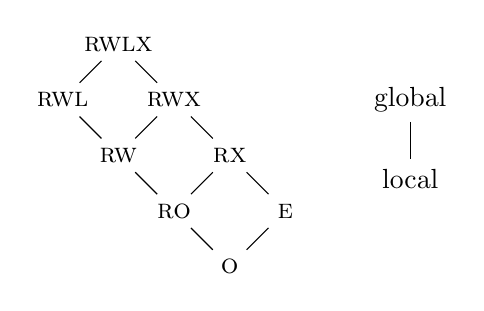
\begin{tikzpicture}[main node/.style={}]
    \node[main node] (7) {$\rwlx$};
    \node[main node] (8) [below left of=7] {$\readwritel$};
    \node[main node] (1) [below right of=7] {$\rwx$};
    \node[main node] (2) [below right of=1] {$\exec$};
    \node[main node] (3) [below right of=2] {$\entry$};
    \node[main node] (4) [below left of=1] {$\readwrite$};
    \node[main node] (5) [below right of=4] {$\readonly$};
    \node[main node] (6) [below right of=5] {$\noperm$};

    \path[every node/.style={font=\sffamily\small}]
    (7) edge (8)
    (7) edge (1)
    (8) edge (4)
    (1) edge (2)
    (2) edge (3)
    (2) edge (5)
    (3) edge (6)
    (1) edge (4)
    (4) edge (5)
    (5) edge (6);

    \node[main node] (1l) [right of=1, xshift=2cm] {$\glob$};
    \node[main node] (2l) [below of=1l] {$\local$};

    \path[every node/.style={font=\sffamily\small}]
    (1l) edge (2l);
  \end{tikzpicture}
  \caption{Permission and locality hierarchy.}
  \label{fig:perm-hier}
\end{wrapfigure}

We define the syntax of our capability machine in \figurename~\ref{fig:syntax}.
We assume an infinite set of addresses $\Addrs$ and define machine words as
either integers or capabilities of the form
$((\perm,\gl),\var{base},\var{end},\addr)$. Such a capability represents the
authority to execute permissions $\perm$ on the memory range
$[\var{base},\var{end}]$, together with a current address $\addr$ and a locality tag
$\gl$ indicating whether the capability is global or local. There is no notion
of pointers other than capabilities, so we will use the terms interchangeably.
The available permissions are null permission
($\noperm$), readonly ($\readonly$), read/write ($\readwrite$), read/execute
($\exec$) and read/write/execute ($\rwx$) permissions. Additionally, there are
three special permissions: read/write-local ($\readwritel$), read/write-local/execute
($\rwlx$) and enter ($\entry$), which we will explain below.
\itoplas{Permissions and locality are ordered and both orderings are depicted in \figurename~\ref{fig:perm-hier}. We denote the pairwise ordering of permission and locality with $\sqsubseteq$.}

We assume a finite set of register names $\RegName$. We define register files
$\reg$ and memories $\ms$ as functions mapping register names resp. addresses to
words. The state of the entire machine is represented as a configuration that is
either a running state $\Phi \in \ExecConfs$ containing a memory and a register file,
or a failed or halted state, where the latter keeps hold of the final state of
memory.
% We also define memory segments $\ms$:
% parts of memory represented as partial functions mapping addresses to words.
%\lau{we don't really make the distinction between memory and memory segments in the rest of the paper, so maybe we should leave this out?}

The machine's instruction set is rather basic. Instructions $i$ include
relatively standard jump ($\jmp{}$), conditional jump ($\jnz{}{}$) and move
($\move{}{}$, copies words between registers) instructions. Also familiar are
load and store instructions for reading from and writing to memory ($\load{}{}$
and $\store{}{}$) and arithmetic operators ($\lt{}{}{}$ (less than), $\plus{}{}{}$ and
$\minus{}{}{}$, operating only on numbers). There are three instructions for
modifying capabilities: $\lea{}{}$ (modifies the current address),
$\restricttwo{}{}$ (modifies the permission and local/global tag) and
$\subseg{}{}{}$ (modifies the range of a capability). Importantly, these
instructions take care that the resulting capability always carries less
authority than the original (e.g. $\restricttwo{}{}$ will only weaken a permission).
Finally, the instruction $\isptr{}{}$ tests whether a word is a capability or a
number and instructions $\getp{}{}$, $\getl{}{}$, $\getb{}{}$, $\gete{}{}$ and
$\geta{}{}$ provide access to a capability's permissions, local/global tag, base,
end and current address, respectively.

\begin{comment}
  \begin{figure}
    \centering
    \begin{mathpar}
      \Phi \rightarrow
      \begin{cases}
        \sem{\decode(n)}(\Phi) & \arraycolsep=0pt
        \begin{array}[t]{l}
          \text{if $\memreg(\pcreg) = \stdcap$}\\
          \;\;\text{and $\start \leq \addr \leq \addrend$ and $\memheap(\addr) = n$}\\
          \;\;\text{and $\perm \in \{ \exec,\rwx, \rwlx \}$} 
        \end{array}\\
        \failed                & \text{otherwise}
      \end{cases}
      \and \updatePcPerm{w} =
      \begin{cases}
        ((\exec,\gl),\start,\addrend,\addr) & \text{\footnotesize{if $w = ((\entry,\gl),\start,\addrend,\addr)$}}\\
        w & \text{otherwise}
      \end{cases}\\
      \and \stdUpdatePc{\Phi} =
      \begin{cases}
        \updateReg{\pcreg}{\var{newPc}} & \arraycolsep=0pt
        \begin{array}[t]{l}
          \text{if $\memreg(\pcreg) = \stdcap$}\\ 
          \;\;\text{and $\var{newPc} = ((\perm,\gl),\start,\addrend,\addr + 1)$}
        \end{array}\\
        \failed & \text{otherwise}
      \end{cases}
      \and \inferrule{ } { \sem{\fail}(\Phi) = \failed } \and
      \inferrule{ } { \sem{\halt}(\Phi) = (\halted,\memheap) } \and
      \inferrule{ } { \sem{\move{\refreg{r_1}}{r_2}}(\Phi) =
        \stdUpdatePc{}(\updateReg{r_1}{\memreg(r_2)}) } \and
      \inferrule{ \memreg(r_2) = \stdcap \\
        \perm \in \{ \rwx, \rwlx, \exec, \readwrite,
        \readwritel, \readonly \}\\
        \start \leq \addr \leq \addrend } {
        \sem{\load{\refreg{r_1}}{\refheap{r_2}}}(\Phi) =
        \updateReg{r_1}{\memheap(\addr)}} \and
      \inferrule{ \memreg(r_2) = \stdcap[\permp]\\
        \permp' = \decodePermPair{\memreg(r_2)}\\
        \permp'\sqsubseteq \permp } {
        \sem{\restricttwo{\refreg{r_1}}{r_2}}(\Phi) = \\
        \stdUpdatePc{}(\updateReg{r_1}{(\permp',\start,\addrend,\addr)})
      } \and \inferrule{ \memreg(r_2) = ((\_,\_),\_,\_,\addr) } {
        \sem{\geta{\refreg{r_1}}{\refreg{r_2}}}(\Phi) =
        \stdUpdatePc{\updateReg{r_1}{\addr}}} \and \inferrule{
        \var{newPc} = \updatePcPerm{\memreg(\lv)} } {
        \sem{\jmp{\lv}}(\Phi) = \updateReg{\pcreg}{\var{newPc}} } \and
      \inferrule{ \memreg(r_1) = \stdcap\\
        \start \leq \addr \leq \addrend\\
        \perm \in \{ \rwx, \rwlx, \readwrite, \readwritel\}\\
        \var{w} = \memreg(r_2) \\
        \var{w} = ((\_,\local),\_,\_,\_)\Rightarrow\perm \in
        \{\rwlx,\readwritel \} } {
        \sem{\store{\refheap{r_1}}{\refreg{r_2}}}(\Phi) =
        \stdUpdatePc{\updateHeap{\addr}{\var{w}}} } \and
    \end{mathpar}
    \caption{An excerpt from the operational semantics.}
    \label{fig:op-sem}
  \end{figure}
\end{comment}
\figurename~\ref{fig:op-sem}
%\itoplassug{Suggestion: extend this figure with more (all?) of the operational semantics. In general, should we add all the missing definitions and make this document closer to being self-contained.} 
shows the operational semantics for a
few representative instructions. Essentially, a configuration $\Phi$ either
decodes and executes the instruction at $\memreg(\pcreg)$ if it is executable
and its address is in the valid range or otherwise fails. The table in the
figure shows for instructions $i$ the result of executing them in configuration
$\Phi$. The instructions $\fail$ and $\halt$ obviously fail and halt respectively. $\move{}{}$
simply modifies the register file as requested and updates the $\pcreg$ to the
next instruction using the meta-function $\stdUpdatePc{}$.

\dominique{Follow order of figure in discussion?}
The $\load{}{}$ instruction loads the contents of the requested memory location
into a register, but only if the capability has appropriate authority (i.e.\
read permission and an appropriate range). $\restricttwo{}{}$ updates a
capability's permissions and global/local tag in the register file, but only if the new permissions are weaker than the original. 
%\itoplassug{Reviewer E, popl, would like $\sqsubseteq$ and $\decodePermPair{}$ explained. If we explain all of these details, this section becaomes a bit long and cluncky. (see tex for suggestion)}
%\itoplassug{As the permissions and global/local tag are not words on the machine, we decode the word in register $r_2$ as a pair of permission and locality which is done with the function $\decodePermPair{}$.}
% Reviewer E, popl: Figure 3: how is decodePermPair defined, and what is the relation between (perm', g') and (perm, g)?
It also never turns local
capabilities into global ones. $\geta{}{}$ queries the current address of a
capability and stores it in a register.

The $\jmp{}$ instruction updates the program counter to a requested location,
but it is complicated by the presence of \emph{enter capabilities}, modeled
after the M-Machine's~\citep{Carter:1994:HSF:195473.195579}. Enter capabilities
cannot be used to read, write or execute and their address and range cannot be
modified. They can only be used to jump to, but when that happens, their
permission changes to $\exec$. They can be used to represent a kind of closures:
an opaque package containing a piece of code together with local encapsulated
state. Such a package can be built as an enter capability $c =
((\entry,\gl),\start,\addrend,\addr)$ where the range $[\start,\addr-1]$
contains local state (data or capabilities) and $[\addr,\addrend]$ contains
instructions. The package is opaque to an adversary holding $c$ but when $c$ is
jumped to, the instructions can start executing and have access to the local
data through the updated version of $c$ that is then in $\pcreg$. 
\lau{As we talked about what is described here, is not how we make closures in
the TR, so we should consider whether we should refrain from using that word
here. }

Finally, the $\store{}{}$ instruction updates the memory to the requested value
if the capability has write authority for the requested location. However, the
instruction is complicated by the presence of \emph{local capabilities}, modeled
after the ones in the CHERI processor~\citep{Watson2015Cheri}. Basically, local
capabilities are special in that they can only be kept in registers, i.e.\ they
cannot be stored to memory. This means that local capabilities can be
\emph{temporarily} given to an adversary, for the duration of an invocation: if
we take care to clear the capability from the register file after control is
passed back to us, they will not have been able to store the capability.
However, there is one exception to the rule above: local capabilities can be
stored to memory for which we have a capability with write-local authority
(i.e.\ permission $\rwl$ or $\rwlx$). This is intended to accommodate a stack,
where register contents can be stored, including local capabilities. As long as
all capabilities with write-local authority are themselves local and the stack
is cleared after control is passed back by the adversary, we will see that this
does not break the intended behavior of local capabilities.

We point out that our local capabilities capture only a part of the semantics of
local capabilities in CHERI. Specifically, in addition to the above, CHERI's
default implementation of the CCall exception handler forbids local capabilities
from being passed across module boundaries. Such a restriction fundamentally
breaks our calling convention, since we pass around local return pointers and
stack capabilities. However, CHERI's CCall is not implemented in hardware, but
in software, precisely to allow experimenting with alternative models like ours.
\dominique{Update to CHERI's new ccall story.}

% Contrary to more traditional assembly languages, capability machines do not 
% allow literal addresses to appear as part of instructions. This means that we

In order to have a reasonably realistic system, we use a simple model of linking
where a program has access to a linking table that contains capabilities for
other programs. We also assume malloc to be part of the trusted computing base
satisfying a certain specification. Malloc and linking tables are described
further in the next section.
\itoplas{The specification of malloc is presented in \sectionname~\ref{sec:malloc} as it uses the semantic model we build in Section~\ref{sec:logical-relation}.
For full details on the linking table, we refer to the technical
appendix~\citep{technical_appendix}.} \itoplas{(Reviewer A, esop suggest explaining the
  linking model)\\}
\itoplassug{Suggestion: We also have the flag table used
  for assertions, maybe we should add a description of it here.\\}
% \itoplassug{Reviewer C, popl, would have liked a discussion of the relationship
%   between this capability machines and old capability machines from the
%   litterature (Cambridge CAP \& IBM System 39, see tex comment).\\}
 % * I'm old, so I'd appreciate a brief discussion LCM's relationship
 %  with the capability hardware I (and perhaps other older readers, or
 %  those outside this precise subfield) are likely to have heard of ---
 %  the Cambridge CAP & IBM System 39.  I think the capabilities of the
 %  machine are not that far from CAP, but this machine has the local
 %  capabilities support. Is that right?


\section{Stack and Return Pointer Management Using Local Capabilities}
\label{sec:stack-and-return-pointer}
\itoplassug{Suggestion: say something about arguments in this paragraph instead of defering it to the discussion only?\\}
\itoplassug{Suggestion: Add some of our presentation illustration figures to illustrate some of the issues? May not be feasible as they rely on ``animation''.\\}
% ## Clarify attacker model earlier
% The proposed calling convention seems able to protect multiple
% components from each other, yet most of the paper discusses this
% protection only in terms of one single statically known
% "adversary". This seems to be selling short the work, and raising
% questions of whether this calling convention is much weaker
% security-wise than the CHERI one, which is clearly about protecting
% multiple components. It would be good to explain this better upfront,
% not just in the discussions section at the end.
\itoplassug{Suggestion: Include a description of (possibly definition for) well-bracketedness? (requested by reviewer C, popl). Reviewer D, popl, asks for the same but also a definition of local state encapsulation. In the POPL notes, I wrote that I talked with Lars about it and this is something that is not easily defined. Perhaps we should have a discussion of this.\\}
One of the contributions in this paper is a
demonstration that local capabilities on a capability machine support a calling
convention that enforces control-flow correctness in a way that is provably
watertight, potentially efficient, does not rely on a trusted central stack
manager and supports higher-order interfaces to an adversary, where an adversary
is just some unknown piece of code. In this section, we explain this
convention's high-level approach, the security measures to be taken in a number
of situations (motivating each separately with a summary table at the end).
After that, we define a number of reusable macro-instructions that can be used
to conveniently apply the proposed convention in subsequent examples.

The basic idea of our approach is simple: we stick to a single, rather standard,
C stack and register-passed stack and return pointers, much like a standard C
calling convention. However, to prevent various ways of misusing this basic
scheme, we put local capabilities to work and take a number of
not-always-obvious safety measures. The safety measures are presented in terms
of what \emph{we} need to do to protect ourselves against an \emph{adversary},
but this is only for presentation purposes as our code assumes no special status on
the machine. In fact, an adversary can apply the same safety measures to protect
themselves against us. In the next paragraphs, we will explain the issues to be
considered in all the relevant situations: when (1) starting our program, (2)
returning to the adversary, (3) invoking the adversary, (4) returning from the
adversary, (5) invoking an adversary callback and (6) having a callback invoked
by the adversary.

\textbf{Program start-up} We assume that the language runtime initializes the
memory as follows: a contiguous array of memory is reserved for the stack, for
which we receive a stack pointer in a special register $r_\stk$. We stress that
the stack is not built-in, but merely an abstraction we put on this piece of the
memory. The stack pointer is local and has $\rwlx$ permission. Note that this
means that we will be placing and executing instructions on the stack.
Crucially, the stack is the only part of memory for which the runtime (including
malloc, loading, linking) will ever provide $\rwlx$ or $\rwl$ capabilities.
Additionally, our examples typically also assume some memory to store
instructions or static data. Another part of memory (called the heap) is
initially governed by malloc and at program start-up, no other code has
capabilities for this memory. Malloc hands out $\rwx$ capabilities for allocated
regions as requested (no $\rwlx$ or $\rwl$ permissions). For simplicity, we
assume that memory allocated through malloc cannot be freed.

\textbf{Returning to the adversary} Perhaps the simplest situation is returning
to the adversary after they invoked our code (\figurename~\ref{fig:illu-intro}). In this case, we have received a
return pointer from them, and we just need to jump to it as usual. An obvious
security measure to take care of is properly clearing the non-return-value
registers before we jump (since they may contain data or capabilities that the
adversary should not get access to). Additionally, we may have used the stack
for various purposes (register spilling, storing local state when invoking other
functions etc.), so we also need to clear that data before returning to the
adversary (\figurename~\ref{fig:illu-priv-data} and \figurename~\ref{fig:illu-clear-priv}).

However, if we are returning from a function that has itself invoked adversary
code (\figurename~\ref{fig:illu-call-adv}), then clearing the used part of the stack is not enough. The \emph{unused}
part of the stack may also contain data and capabilities, left there by the
adversary, including local capabilities since the stack is write-local. As we
will see later, we rely on the fact that the adversary cannot keep hold of local
capabilities when they pass control to the trusted code and receive control
back. In this case, the adversary could use the unused part of the stack to
store local pointers and load them from there after they get control back (\figurename~\ref{fig:illu-adv-data}). To
prevent this, we need to clear (i.e.\ overwrite with zeros) the entire part of
the stack that the adversary has had access to, not just the parts that we have
used ourselves (\figurename~\ref{fig:illu-clear-all}). Since we may be talking about a large part of memory, this
requirement is the most problematic aspect of our calling convention for
performance, but see \sectionname~\ref{sec:discussion} for how this might be
mitigated.

\begin{figure}[htb]
  \centering
  \begin{subfigure}{0.32\linewidth}
    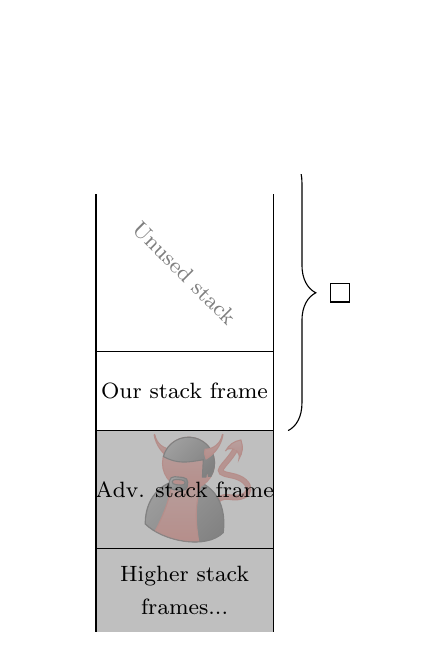
\begin{tikzpicture}[scale=.5, every node={scale=.5}]
    % recurrent parts
    \stdstackstart

    % attacker ..
      \inactadv{(0,2)}{(4.5,5)}{Adv. stack frame}

    % trusted stack frame
      \actsf{(0,5)}{(4.5,7)}{Our stack frame}

    % Unused part
      \node[opacity=0.5,rotate=-45] at (2.25,9) {\footnotesize Unused stack};

      % Stack pointer
      \begin{scope}
        \clip (4.6,5) rectangle (7.6,11.5);
        \capbrace{(4.6,5)}{(4.6,12)}{sp}
      \end{scope}
    \end{tikzpicture}
    \caption{}
  \label{fig:illu-intro}
  \end{subfigure}
  \begin{subfigure}{0.333\linewidth}
    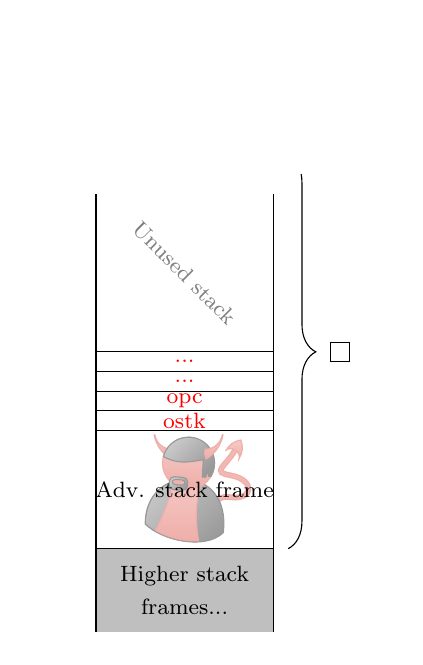
\begin{tikzpicture}[scale=.5, every node={scale=.5}]
    % recurrent parts
    \stdstackstart

    % attacker ..
      \actadv{(0,2)}{(4.5,5)}{Adv. stack frame}

    % trusted stack frame
      \actsf{(0,5)}{(4.5,7)}{Our stack frame}
      \draw[fill=white] (0,5) rectangle (4.5,5.5) node[pos=.5,color=red] {\footnotesize ostk};
      \draw[fill=white] (0,5.5) rectangle (4.5,6) node[pos=.5,color=red] {\footnotesize opc};
      \draw[fill=white] (0,6) rectangle (4.5,6.5) node[pos=.5,color=red] {\footnotesize ...};
      \draw[fill=white] (0,6.5) rectangle (4.5,7) node[pos=.5,color=red] {\footnotesize ...};


    % Unused part
      \node[opacity=0.5,rotate=-45] at (2.25,9) {\footnotesize Unused stack};

      % Stack pointer
      \begin{scope}
        \clip (4.6,2) rectangle (7.6,11.5);
        \capbrace{(4.6,2)}{(4.6,12)}{sp}
      \end{scope}
    \end{tikzpicture}
  \caption{}
  \label{fig:illu-priv-data}
  \end{subfigure}
  \begin{subfigure}{0.333\linewidth}
    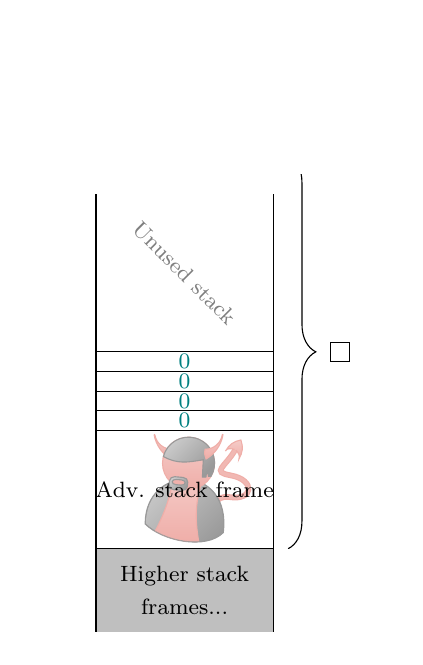
\begin{tikzpicture}[scale=.5, every node={scale=.5}]
    % recurrent parts
    \stdstackstart

    % attacker ..
      \actadv{(0,2)}{(4.5,5)}{Adv. stack frame}

    % trusted stack frame
      \actsf{(0,5)}{(4.5,7)}{Our stack frame}
      \draw[fill=white] (0,5) rectangle (4.5,5.5) node[pos=.5,color=teal] {\footnotesize 0};
      \draw[fill=white] (0,5.5) rectangle (4.5,6) node[pos=.5,color=teal] {\footnotesize 0};
      \draw[fill=white] (0,6) rectangle (4.5,6.5) node[pos=.5,color=teal] {\footnotesize 0};
      \draw[fill=white] (0,6.5) rectangle (4.5,7) node[pos=.5,color=teal] {\footnotesize 0};


    % Unused part
      \node[opacity=0.5,rotate=-45] at (2.25,9) {\footnotesize Unused stack};

      % Stack pointer
      \begin{scope}
        \clip (4.6,2) rectangle (7.6,11.5);
        \capbrace{(4.6,2)}{(4.6,12)}{sp}
      \end{scope}
    \end{tikzpicture}
  \caption{}
  \label{fig:illu-clear-priv}
  \end{subfigure}


  \begin{subfigure}{0.32\linewidth}
    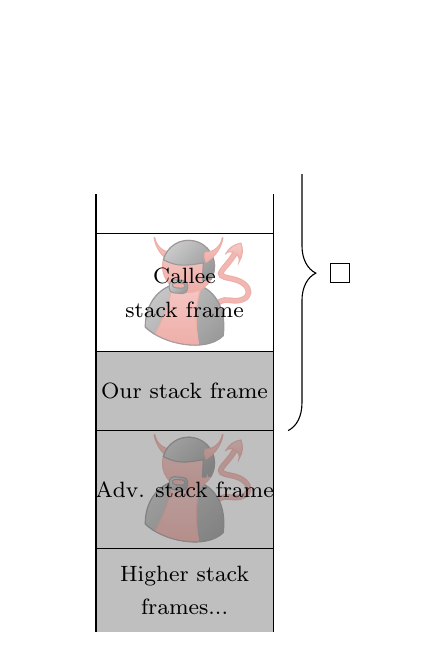
\begin{tikzpicture}[scale=.5, every node={scale=.5}]
    % recurrent parts
    \stdstackstart

    % attacker ..
      \inactadv{(0,2)}{(4.5,5)}{Adv. stack frame}

    % trusted stack frame
      \inactsf{(0,5)}{(4.5,7)}{Our stack frame}

    % second attacker
      \actadv{(0,7)}{(4.5,10)}{Callee\\\footnotesize stack frame}


      % Stack pointer
      \begin{scope}
        \clip (4.6,5) rectangle (7.6,11.5);
        \capbrace{(4.6,5)}{(4.6,13)}{sp}
      \end{scope}
    \end{tikzpicture}
  \caption{}
  \label{fig:illu-call-adv}
  \end{subfigure}
  \begin{subfigure}{0.333\linewidth}
    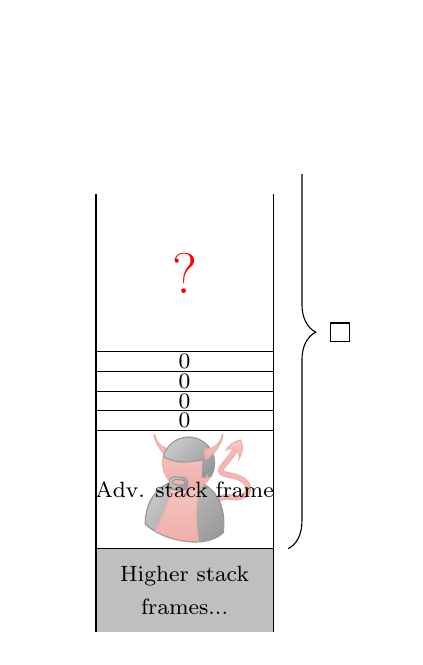
\begin{tikzpicture}[scale=.5, every node={scale=.5}]
    % recurrent parts
    \stdstackstart

    % attacker ..
      \actadv{(0,2)}{(4.5,5)}{Adv. stack frame}

    % trusted stack frame
      \actsf{(0,5)}{(4.5,7)}{Our stack frame}
      \draw[fill=white] (0,5) rectangle (4.5,5.5) node[pos=.5] {\footnotesize 0};
      \draw[fill=white] (0,5.5) rectangle (4.5,6) node[pos=.5] {\footnotesize 0};
      \draw[fill=white] (0,6) rectangle (4.5,6.5) node[pos=.5] {\footnotesize 0};
      \draw[fill=white] (0,6.5) rectangle (4.5,7) node[pos=.5] {\footnotesize 0};

    % Unknown part
      \node[color=red] at (2.25,9) {\huge ?};

      % Stack pointer
      \begin{scope}
        \clip (4.6,2) rectangle (7.6,11.5);
        \capbrace{(4.6,2)}{(4.6,13)}{sp}
      \end{scope}
    \end{tikzpicture}
  \caption{}
  \label{fig:illu-adv-data}
  \end{subfigure}
  \begin{subfigure}{0.333\linewidth}
    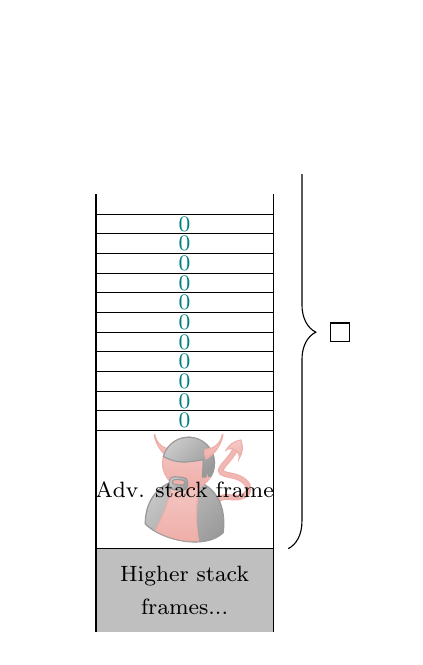
\begin{tikzpicture}[scale=.5, every node={scale=.5}]
    % recurrent parts
    \stdstackstart

    % attacker ..
      \actadv{(0,2)}{(4.5,5)}{Adv. stack frame}

    % trusted stack frame
      \actsf{(0,5)}{(4.5,7)}{Our stack frame}
      \foreach \x in {5,5.5,...,10}
      {
        \draw[fill=white] (0,\x) rectangle (4.5,\x+.5) node[pos=.5,color=teal] {\footnotesize 0};
      };

      % Stack pointer
      \begin{scope}
        \clip (4.6,2) rectangle (7.6,11.5);
        \capbrace{(4.6,2)}{(4.6,13)}{sp}
      \end{scope}
    \end{tikzpicture}
  \caption{}
  \label{fig:illu-clear-all}
  \end{subfigure}
  \caption{Illustration of the situations related to stack clearing when returning to an adversary.
    The greyed out areas are parts of the stack that are not accessible at the time.}
  \label{fig:ret-adv}
\end{figure}
\textbf{Invoking the adversary} A slightly more complex case is invoking the
adversary. As above, we clear all the non-argument registers, as well as the
part of the stack that we are not using (because, as above, it may contain local
capabilities from previously executed code that the adversary could exploit in
the same way). We leave a copy of the stack pointer in $r_\stk$, but only after
we have used the $\subseg{}{}{}$ instruction to shrink its authority to the part
that we are not using ourselves.

In one of the registers, we also provide a return pointer, which must be a local
capability. If it were global, the adversary would be able to store away the
return pointer in a global data structure (i.e.\ there exists a global capability for it), and jump to it later, in
circumstances where this should not be possible. For example, they could store
the return pointer, legally jump to it a first time, wait to be invoked again
and then jump to the old return pointer a second time, instead of the new return
pointer received for the second invocation. Similarly, they could store the
return pointer, invoke a function in our code, wait for us to invoke them again
and then jump to the old return pointer rather than the new one, received for the
second invocation.
% \lau{If we need space, then maybe one of the examples is sufficient.}
% \lau{Both of these are good to have their as the two last examples of \sectionname~\ref{sec:examples} use them.}
%
% \lau{In the examples, we refer to the local return pointer as
%   ``protected return pointer''. We should either introduce that here
%   or use a different formulation in the examples. }
% \lau{It seemed did not seem to add anything to adopt the terminlogy - we
%   often highlight that the return pointer is local which in most cases
%   is so important that we do not want to leave it out.}
By making the return pointer local, we prevent such attacks: the adversary can
only store local capabilities through write-local capabilities, which means (because
of our assumptions above): on the stack. Since the stack pointer itself is
also local, it can also only be stored on the stack. Because we clear the part
of the stack that the adversary has had access to before we pass control back,
there is no way for them to recover either of these local capabilities.

Note that storing stack pointers for use during future invocations would also be
dangerous in itself, i.e. not just because it can be used to store return
pointers. Imagine the adversary stores their stack pointer (\ref{fig:illu-adv-store-sp}), invokes trusted code
that uses part of the stack to store private data (\ref{fig:illu-adv-call}) and then invokes the adversary
again with a stack pointer restricted to exclude the part containing the private
data (\ref{fig:illu-adv-called}). If the adversary had a way of keeping hold of their old stack pointer, it
could access the private data stored there by the trusted code and break
local-state encapsulation.  
% \lau{Do we say anything about arguments to the callback? Specifically, it should not be okay to uncritically pass on argument we recieved from an adversary. Can we even to any extend allow local arguments that we pass on from an unknown source?}
% Domi: this is now discussed in the discussion section, no need to discuss it here?

\begin{figure}[htb]
  \centering
  \begin{subfigure}{0.32\linewidth}
    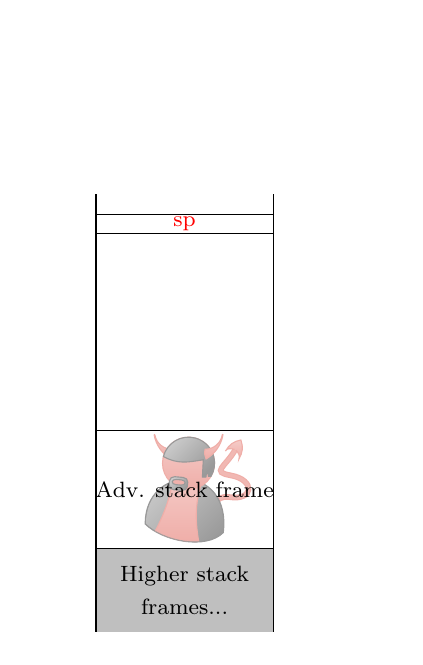
\begin{tikzpicture}[scale=.5, every node={scale=.5}]
    % recurrent parts
    \stdstackstart

    % attacker ..
      \actadv{(0,2)}{(4.5,5)}{Adv. stack frame}
      \draw[fill=white] (0,10) rectangle (4.5,10.5) node[pos=.5,color=red] {\footnotesize sp};
    % Stack pointer
      \begin{scope}
        \clip (4.6,2) rectangle (7.6,11.5);
        \capbracebot{(4.6,2)}{(4.6,12)}{sp}
      \end{scope}
    \end{tikzpicture}
    \caption{}
  \label{fig:illu-adv-store-sp}
  \end{subfigure}
  \begin{subfigure}{0.333\linewidth}
    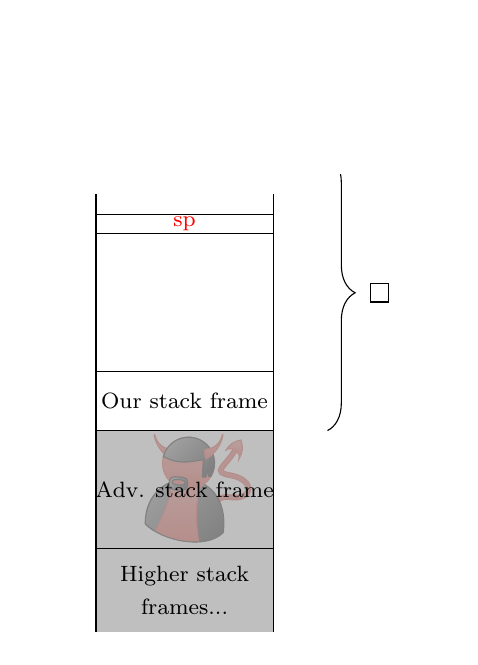
\begin{tikzpicture}[scale=.5, every node={scale=.5}]
    % recurrent parts
    \stdstackstart

    % attacker ..
      \inactadv{(0,2)}{(4.5,5)}{Adv. stack frame}
      \draw[fill=white] (0,10) rectangle (4.5,10.5) node[pos=.5,color=red] {\footnotesize sp};

    % Our stack frame
      \actsf{(0,5)}{(4.5,6.5)}{Our stack frame}

    % Stack pointer
      \begin{scope}
        \clip (4.6,2) rectangle (7.6,11.5);
        \capbracebotred{(4.6,2)}{(4.6,12)}{sp}
      \end{scope}
      \begin{scope}
        \clip (5.6,5) rectangle (9,11.5);
        \capbrace{(5.6,5)}{(5.6,12)}{sp'}
      \end{scope}

    \end{tikzpicture}
  \caption{}
  \label{fig:illu-adv-call}
  \end{subfigure}
  \begin{subfigure}{0.333\linewidth}
    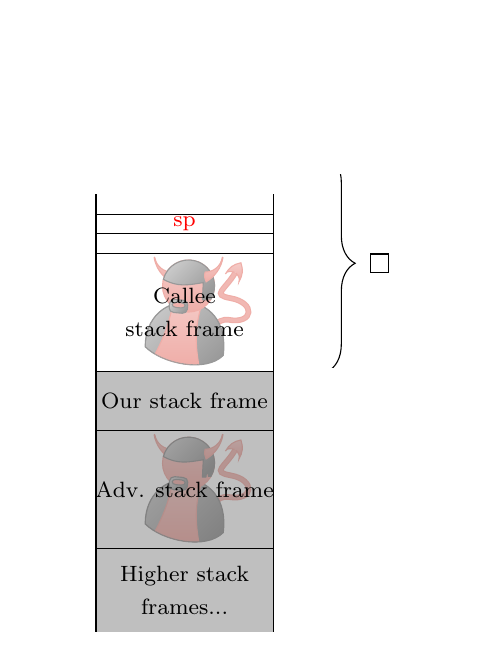
\begin{tikzpicture}[scale=.5, every node={scale=.5}]
    % recurrent parts
    \stdstackstart

    % attacker ..
      \inactadv{(0,2)}{(4.5,5)}{Adv. stack frame}

    % Stored stack pointer
      \draw[fill=white] (0,10) rectangle (4.5,10.5) node[pos=.5,color=red] {\footnotesize sp};

    % Our stack frame
      \inactsf{(0,5)}{(4.5,6.5)}{Our stack frame}

    % Second attacker
      \actadv{(0,6.5)}{(4.5,9.5)}{Callee \\ \footnotesize stack frame}

    % Stack pointer
      \begin{scope}
        \clip (4.6,2) rectangle (7.6,11.5);
        \capbracebotred{(4.6,2)}{(4.6,12)}{sp}
      \end{scope}
      \begin{scope}
        \clip (5.6,6.6) rectangle (9,11.5);
        \capbrace{(5.6,6.5)}{(5.6,12)}{sp'}
      \end{scope}
    \end{tikzpicture}
  \caption{}
  \label{fig:illu-adv-called}
  \end{subfigure}
  \caption{Illustration of the situations related to stack clearing when invoking an adversary.
    The greyed out areas are parts of the stack that are not accessible at the time.
  }
  \label{fig:invoke-adv}
\end{figure}


\textbf{Returning from the adversary} So return pointers must be passed as local
capabilities. But what should their permissions be, what memory should they
point to and what should that memory (the activation record) contain? Let us
answer the last question first by considering what should happen when the
adversary jumps to a return pointer. In that case, the program counter should be
restored to the instruction after the jump to the adversary, so the activation
record should store this old program counter. Additionally, the stack pointer
should also be restored to its original value. Since the adversary has a more
restricted authority over the stack than the code making the call, we cannot
hope to reconstruct the original stack pointer from the stack pointer owned by the
adversary. Instead, it should be stored as part of the activation record.

\begin{figure}[htb]
  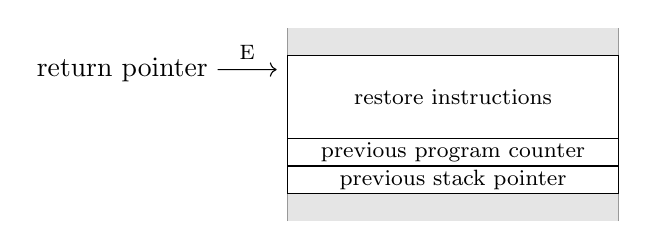
\begin{tikzpicture}[scale=.7, every node={scale=.7}]
    \draw[fill=gray!20,draw=none] (0,4) rectangle (6,3.5);
    \draw[fill=gray!20,draw=none] (0,0.5) rectangle (6,1);
    \draw[draw=gray!80] (0,0.5) -- (0,4);
    \draw[draw=gray!80] (6,0.5) -- (6,4);
    \draw (0,1) rectangle (6,1.5) node[pos=.5] {\footnotesize previous stack pointer};
    \draw (0,1.5) rectangle (6,2) node[pos=.5] {\footnotesize previous program counter};
    \draw (0,2) rectangle (6,3.5) node[pos=.5] {\footnotesize restore instructions};
    \draw (-3,3.25) node (rp) {return pointer};
    \draw[->] (rp.east) -- node[above] {$\entry$}(-.2,3.25);
  \end{tikzpicture}
  
  \caption{Structure of an activation record}
  \label{fig:activ-rec-struct}
\end{figure}

Clearly, neither of these capabilities should be accessible by the adversary. In
other words, the return pointer provided to the adversary must be a capability
that they can jump to but not read from, i.e.\ an enter capability. To make this
work, we construct the activation record as depicted in
\figurename~\ref{fig:activ-rec-struct}. The $\entry$ return pointer has authority
over the entire activation record (containing the previous return and stack
pointer), and its current address points to a number of restore instructions in
the record, so that upon invocation, these instructions are executed and can
load the old stack pointer and program counter back into the register file. As
the return pointer is an enter pointer, the adversary cannot get hold of the
activation record's contents, but after invocation, its permission is updated to
$\exec$, so the contents become available to the restore instructions.

The final question that remains is: where should we store this activation
record? The attentive reader may already see that there is only one possibility:
since the activation record contains the old stack pointer, which is local, the
activation record can only be constructed in a part of memory where we have
write-local access, i.e.\ on the stack. Note that this means we will be placing
and executing instructions on the stack, i.e.\ it will not just contain code
pointers and data. This means that our calling convention should be combined
with protection against stack smashing attacks (i.e.\ buffer overflows on the
stack overwriting activation records' contents). Luckily, the capability
machine's fine-grained memory protection should make it reasonably easy for a
compiler to implement such protection, by making sure that only appropriately
bounded versions of the stack pointer are made available to source language
code.

\textbf{Invoking an adversary callback} If we have a higher-order interface to
the adversary, we may need to invoke an adversary callback. In this case, not so
much changes with respect to the situation where we invoke static adversary
code. The adversary can provide a callback as a capability for us to jump to,
either an $\entry$-capability if they want to protect themselves from us or just
an $\exec$ capability if they are not worried about that. However, there is one
scenario that we need to prevent: if they construct the callback capability to
point into the stack, it may contain local capabilities that they should not
have access to upon invocation of the callback. As before, this includes return
and stack pointers from previous stack frames that they may be
trying to illegally use inside the callback.

To prevent this, we only accept callbacks from the adversary in the form of
global capabilities, which we dynamically check before invoking them (and we
fail otherwise). This should not be an overly strict requirement: our own
callbacks do not contain local data themselves, so there should be no need for
the adversary to construct callbacks on the stack.\footnote{Note that it does
  prevent a legitimate but non-essential scenario where the adversary wants to
  give us temporary access to a callback not allocated on the stack.}
\itoplassug{Maybe a word on arguments passed from the adversary to us that we pass on to a callback given by the adversary (mentioned by reviewer E, popl, see tex comment.)}
%page 8: "we only accept callbacks from the adversary in the form of global capabilities, which we dynamically check before invoking them".  This makes sense, but don't you also need to check arguments that are passed from the adversary to us and then passed by us into the callback?


\textbf{Having a callback invoked by the adversary} The above leaves us with
perhaps the hardest scenario: how to provide a callback to the adversary. The
basic idea is that we allocate a block of memory using malloc that we fill with
the capabilities and data that the callback needs, as well as some
prelude instructions that load the data into registers and jumps to the right
code. Note that this implies that no local capabilities can be stored as part of
a closure. We can then provide the adversary with an enter-capability covering
the allocated block and pointing to the contained prelude instructions. However,
the question that remains in this setup is: from where do we get a stack pointer when
the callback is invoked?

Our answer is that the adversary should provide it to us, just as we provide
them with a stack pointer when we invoke their code. However, it is important
that we do not just accept any capability as a stack pointer but check that it
is safe to use. Specifically, we check that it is indeed an $\rwlx$ capability. Without
this check, an adversary could potentially get control over our local stack
frame during a subsequent callback by passing us a local $\rwx$ capability to a global data
structure instead of a proper stack pointer
and a global callback for our callback to invoke. If our local state contains no
local capabilities, then, otherwise following our calling convention, the callback would
not fail and the adversary could use a stored capability for the global data
structure to access our local state. To prevent this from happening, we need to
make sure the stack capability carries $\rwlx$ authority, since the system wide assumption then
tells us that the adversary cannot have global capabilities to our local stack.

\textbf{Calling convention} With the security measures introduced and motivated,
let us summarize our proposed calling convention:
\begin{description}[font=\normalfont\itshape]
\item[At program start-up] A
local $\rwlx$ stack pointer resides in register $r_\stk$. No global write-local capabilities.
\item[Before returning to the adversary] Clear non-return-value
registers. Clear the part of the stack we had access to (not just the part we used).
\item[Before invoking the adversary] Push activation record to the
stack. Create return pointer as local $\entry$-capability to the instructions in
the record.  Restrict the stack capability to the unused part and clear
it. Clear non-argument registers.
\item[Before invoking an adversary callback] Make sure callback is global.
  \item[When invoked by an adversary] Make sure received stack pointer has permission $\rwlx$.
\end{description}

%\itoplassug{Suggestion: Make it more clear that this CC can be used to protect multiple components (reviewer A, ESOP), see tex comment.\\}
\begin{toplas}
  \textbf{Modularity} The calling convention ensures well-bracketed calls and
  local-state encapsulation for the caller, but not the callee. In the above
  presentation to make it easy to distinguish between the parties involved, we
  present the callee as some adversarial code that we do not trust. In reality,
  the callee could be well-behaved and wish to ensure well-bracketed calls and
  local-state encapsulation as well. The calling convention puts no restriction
  on the callee that the caller itself does not follow, so by following the
  calling convention, the callee can also obtain those guarantees. In other
  words, the calling convention is modular and scales to scenarios with multiple
  distrusting parties invoking each other.
\end{toplas}

\section{Logical Relation}
\label{sec:logical-relation}
\itoplassug{Suggestions for things to add heres
  \begin{itemize}
  \item (The lemma is there, consider pointer) Double monotonicity lemma (lemma 77 and 79) with a pointer back to local capability section of popl intro to this section.
  \item Reviewer B, ESOP suggests inferring general security properties from the LR. We had a section in the discussion that explained why this was not really possible. I have reintroduced it in the discussion.
  \end{itemize}
}

% In this section, we formalize the guarantees provided by the
% capability machine, including the specific guarantees for local
% capabilities, by means of a step-indexed Kripke logical relation 
% with recursively defined worlds. 
% We use the logical relation in the following section to show
% local-state encapsulation and control-flow integrity properties for
% challenging example programs.

\begin{toplas}
%\todo[inline]{Look this introduction and the following section through to check for overlap. Also consider making backwards references to this introduction from the places where we use advanced techniques, so it becomes clear that they are necessary.}
% Our logical relation will prescribe which values are capability safe given a
% world $W$ containing a set of memory invariants. For expressiveness,
% we use invariants which can evolve over time (sometimes also referred
% to as \emph{protocols}). We thus start by describing the worlds we
% will use.
Now that we have defined our calling convention, how can we be sure that it
works? More concretely, suppose that we have a program that uses the convention
in its interaction with untrusted adversary code. Can we formally prove the
program's correctness if it relies on well-bracketed control flow and private
state encapsulation for the interaction with the adversary? Clearly, such a
proof should depend on a formal expression of the guarantees provided by the
capability machine, including the specific guarantees for local capabilities.

In this section, we construct such a formalization. We make use of some
well-studied and powerful (but non-trivial) machinery from the literature.
Specifically, we employ a unary step-indexed Kripke logical relation with
recursive worlds, and some additional special characteristics of our own.
Step-indexing, Kripke logical relations and recursive worlds are techniques that
may be familiar from lambda calculus settings, but it may not be clear to the
reader how they apply in this more low-level assembly language. Therefore, in the next section, we do
not immediately dive into the details, but we first try to provide some informal
intuition about how all of this machinery comes into play in our setting.

Note: even though the calling convention is the main application in this paper,
the logical relation we construct is very general and should be regarded as an
independent contribution.

\subsection{Formalizing the guarantees of the capability machine}
\label{sec:formalizing-guarantees}
What differentiates a capability machine from a more standard assembly language
is that we can bound the authority of an executing block of code, based solely
on the capabilities it has access to. Specifically, it does not matter which
instructions are actually executed, i.e., the bound also applies to untrusted
adversary code that has not been inspected or modified in any way.

\paragraph{Worlds}
But what does a ``bound on the authority'' of an executing block of code mean?
In our setting, there are no externally observable side-effects and the only
primitive authority that code may hold is authority over memory. As such, the
authority bounds we consider are related to memory, but in a form that is more
fine-grained than standard read/write authority: a piece of code's authority can be bounded
by arbitrary memory invariants that it is required to respect. Specifically, we
will define worlds $W \in \Worlds$, which describe a set of memory invariants, and
our results will express authority bounds on code as \emph{safety with respect to such
a world,} i.e., the fact that the code respects the invariants registered in
the world.

\paragraph{Safe values}
So, let's say that we have a world $W$ expressing that the memory must contain
value $42$ at address $0$, may contain arbitrary values at
addresses $50$-$60$, a $\readwrite$ capability for address $0$ at address $73$, and
an integer at address $100$ that may only increase over time\footnote{Indeed, we
  will allow a notion of \emph{evolvable} invariants, aka \emph{protocols}, that can
  express such a temporal property.}. Our main theorem will state that if the
current register file only contains safe words (numbers or capabilities which
preserve the invariants in $W$ under any interaction), then an execution will
necessarily also preserve the memory invariants (irrespective of the instructions being
executed).

To make this more precise, we need to define the set $\stdvr(W) \in
\powerset{\Words}$ of words that are safe w.r.t.\ $W$. Essentially, the set
should only include words that preserve $W$'s invariants under any interaction,
but should otherwise be as liberal as possible. Numbers are clearly always safe,
as they cannot be used to break invariants. Whether a capability is safe depends
on the authority that it carries. In the above-described world, a read capability
for address $0$ is safe, as it can only be used to read the value $42$, which is
itself safe. However, a write capability for address $0$ is not safe: it can be
used to overwrite the memory at that address with a value other than $42$,
breaking the invariant for that address.

\paragraph{Step-indexing}
More generally, we want to define that a read capability for memory range
$[b,e]$ is safe, if the world guarantees that the words at those addresses are
themselves safe. However, this definition is cyclic: what if the world
guarantees that the memory at address $a$ will contain a read capability for
address $a$? The definition then just says that a read capability for address
$a$ is safe if and only if the same read capability for address $a$ is safe. This form of
cyclic reasoning is related to similar challenges in languages with recursive
types or higher-order ML-style references, and a standard solution is
to use step-indexing \citep{Appel:2001:IMR:504709.504712}: essentially, the cycle is broken by defining safety up to a
certain number of interaction steps. All words will be considered
safe up to $0$ steps (since if there is no interaction, nothing unsafe
can happen), and, for example, a read capability will be safe up to $n$
steps if the world guarantees that the words at the corresponding addresses are
safe up to $n - 1$ steps. We can then prove that the above read capability for
address $a$ is safe up to any number of steps.

\paragraph{Future worlds}
So worlds are defined as a set of invariants on the memory, but what if we
allocate fresh memory through malloc? We may want to establish new invariants
for this freshly allocated memory and be sure that the adversary will also
respect those (if we don't provide them with capabilities through which the new
invariants can be broken). To accommodate this, we allow worlds to evolve, for
example by adding additional invariants for freshly allocated memory. Formally,
we define valid ways for a world $W$ to evolve into a new world $W'$ through a
future-world relation $W' \future W$ and we ensure that the set of safe words in
world $W$ must remain safe in any future world $W'$. Defining safety w.r.t.\ a
notion of evolvable worlds makes our logical relation into a \emph{Kripke}
logical relation \citep{pitts_operational_1998}.

\paragraph{Invariants and Recursive Worlds}
So worlds group a set of memory invariants, but how are they actually
defined formally? We represent each invariant by a region
$r \in \Regions$. We will see later that regions contain state
machines to support a notion of evolvable invariants, but in every
state, they also contain a predicate $H$ that defines which memory
segments are acceptable in the current state of the invariant.
Unfortunately, it is not enough to just take
$H \in \powerset{\MemSegments}$, because sometimes the invariant may
itself be world-dependent. For example, we may want to express
invariants like ``the memory at address $50$ contains a value that is
safe in the current world''. As explained, worlds may evolve, and the
set of safe values may grow in future worlds, and therefore we need to
index $H$ over worlds, i.e., take
$H \in \Worlds \rightarrow \powerset{\MemSegments}$. We then end up
with worlds containing regions with world-indexed predicates,
i.e., the set of worlds must be recursively defined. We will see how such a recursive
definition can be accommodated using techniques from the
literature (essentially an advanced application of step-indexing).

\paragraph{Local capabilities}
A final thing we provide informal intuition for is how our results take into account local
capabilities and their special treatment by the hardware. Normally, when we
invoke an untrusted piece of code and provide it with certain global
capabilities, it may have stored those capabilities in memory and we will only
be able to reinvoke the code if we can guarantee that those values are still
valid. Formally, worlds represent the invariants that global capabilities'
safety relies on and the reinvocation is only safe in future worlds, where the
invariants are respected.

However, if we provide the adversary with local capabilities in that first
invocation, then the situation is a bit different. The adversary has no way to
store these local capabilities, so if we make sure that there are also no old
local capabilities in the register file for the second invocation (including the
capability being invoked), then the adversary cannot use them any more.%
\footnote{We are ignoring write-local capabilities in this discussion. If the
  adversary does have access to write-local capabilities in the first and second
  invocation, then the memory they address must entirely be cleared before the
  second invocation in order for the reinvocation to remain safe.} Therefore, we
can allow the second invocation to happen in \emph{private} future worlds ($W'
\futurestr W$), in which safe global capabilities remain safe, but local ones
don't. This private future world relation is more liberal than the standard,
public one ($W' \futurewk W$, in which \emph{all} safe capabilities remain
safe). Concretely, worlds may contain \emph{temporary} regions, representing
invariants that only local capabilities may rely on for their safety, and which
may be revoked (disabled) in private future worlds.

Interestingly, this idea is a variant of a notion of public/private future
worlds that has been previously used in the literature (see
\sectionname~\ref{sec:discussion}). However, temporary regions are new in our setting
and there is an interesting interplay with the recursiveness of the worlds: for
a temporary region, the predicate $H \in \Worlds \rightarrow
\powerset{\MemSegments}$ (which defines the safe memory segments in the
current world) is only required to be monotone w.r.t.\ public
future worlds (i.e.\ safe memory segments remain safe in public future worlds),
but for permanent regions, it must be monotone w.r.t.\ private future worlds.
As a consequence, the memory for a permanent region may not contain local
capabilities (as their safety would be broken in private future worlds), which
in turn implies that only local capabilities may have write-local permission (a
general sanity requirement when using local capabilities\footnote{In fact, local
  capabilities become useless as soon as the adversary has access to a single
  global, write-local capability.})\footnote{For explanation purposes, this
  discussion ignores certain ways to allow for local capabilities in a permanent
  region, for example, by not requiring that they are valid or requiring that
  they are local versions of valid global capabilities.}.
\end{toplas}
\subsection{Worlds}
\label{subsec:worlds}
\begin{figure}[htb]
  \centering
  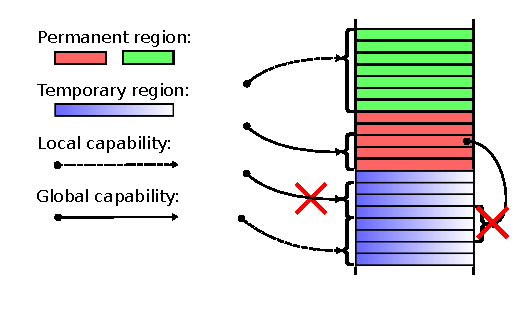
\includegraphics{w11}

  \caption{The relation between local/global capabilities and temporary/permanent
    regions. The colored fields are regions governing parts of memory. Global capabilities cannot depend on temporary
    regions.}
  \label{fig:cap-world}
\end{figure}
% \dominique{Perhaps we could first try to convey the intuition of a permanent
%   world with a temporary overlay, with global capabilities ignoring the overlay.
%   Perhaps we could add a depiction of the world to Figure 5?}
%\todo[inline]{Find a good place to describe monotonicity of
%interpretation function.}
% \lau{this may not be an important enough point to include it.}

%As describe above, worlds are a collection of invariants. Formally, 

A world is a
finite map from region names, modeled as natural numbers, to regions that each
correspond to an invariant of part of the memory.  We have three types of
regions: \emph{permanent}, \emph{temporary}, and \emph{revoked}.
%$\perma$, $\temp$, and $\revoked$. The
%$\perma$ and $\temp$ 
Each permanent and temporary region contains a state transition system, with
public and private transitions, to describe how the invariants are allowed to
change over time. In other words, they are protocols for the region's
memory. Protocols
imposed by permanent regions stay in place indefinitely. Any capability, local
or global, can depend on these protocols. Protocols imposed by temporary regions
can be revoked in private future worlds. Doing this may break the safety of
local capabilities but not global ones. This means that local capabilities
can safely depend on the protocols imposed by temporary regions, but global
capabilities cannot, since a global capability may outlive a temporary region
that is revoked. This is illustrated in \figurename~\ref{fig:cap-world}.

For technical reasons, we do not actually remove a revoked temporary region from
the world, but we turn it into a special revoked region that exists for this purpose.
Such a revoked region contains no state transition system and puts no
requirements on the memory. It simply serves as a mask for a revoked temporary
region. Masking a region like this goes back to earlier work of \citet{Ahmed2004semantics} and was also used by \citet{Thamsborg:2011:KLR:2034773.2034831}.

% Recursive worlds intuition
% The worlds end up being defined recursively: The memory can contain
% capabilities,
% which grant authority over parts of memory. A world
% models memory, so it also needs to be able to model capabilities in
% memory and the protocols on them. Whether a capability satisfies the
% protocol of a region may depend on what it grants authority over in
% memory which is described by the world.

%\dominique{``end up being defined recursively'' does not sound very insightful}
% A region defines what its part of memory can legally look like. However,
% validity of the memory's contents may itself depend on the state of other parts
% of memory. To accommodate this, worlds need to be defined recursively: Worlds
% describe memory, which can contain capabilities, whose safety is
% world-dependent. 
%As described in \sectionname~\ref{sec:formalizing-guarantees}, regions define sets of

Regions are used to define safe memory segments, but this set may itself be world-dependent. In other
words, our worlds are defined recursively. Recursive worlds are common
in Kripke models and the following lemma uses the method of
\citet{Birkedal:2011:SKM:1926385.1926401,Birkedal:tutorial-notes} for
constructing them. The formulation of the lemma is technical, so we recommend
that non-expert readers ignore the technicalities and accept that there exists a
set of worlds $\Wor$ and two relations $\futurestr$ and $\futurewk$ satisfying
the (recursive) equations in the theorem (where the $\blater$ operator can be
safely ignored).
% Short technical explanation
% The recursiveness of the worlds gives rise to a recurisve domain
% equation. Theorem~\ref{thm:world-existence} gives the solution to this
% recursive domain equation.
% \dominique{it is not explained what cofes are?}
% \lau{I added what cofe means but no formal definition (I think this goes under the category technicalities)}
\begin{theorem}\label{thm:world-existence}
  There exists a \cofe{} (complete ordered family of equivalences) $\Wor$ and preorders $\futurestr$ and
  $\futurewk$ such that $(\Wor,\futurestr)$ and $(\Wor,\futurewk)$ are
  preordered \cofes{}, and there exists an isomorphism $\xi$ such that
  \begin{align*}
      \xi \; : \; & \Wor \cong \blater (\nats \finparfun \Regions)\\
      \Regions  = & \; \{\revoked\} \uplus \\
               & \; \{\temp\} \times \States \times \Rels \times (\States \fun (\Wor \monwknefun \UPred{\HeapSegments}))\uplus \\
               & \; \{\perma\} \times \States \times \Rels \times (\States \fun (\Wor \monstrnefun \UPred{\HeapSegments}))
    \end{align*}
  and for $W, W' \in \Wor\ldotp \quad  
  \begin{aligned}
    W' \futurestr W & \Leftrightarrow \xi(W') \futurestr \xi(W)   \\
    W' \futurewk W & \Leftrightarrow \xi(W') \futurewk \xi(W)
  \end{aligned}$
\end{theorem}
In the above theorem, $\States \times \Rels$ corresponds to the aforementioned
state transition system where $\Rels$ contains pairs of relations corresponding
to the public and private transitions, and $\States$ is an unspecified set that
we assume to contain at least the states we use in this paper. The last part of
the temporary and permanent regions is a state interpretation function that
determines what memory segments the region permits in each state of the state
transition system.  The different monotonicity requirements in the two
interpretation functions reflects how permanent regions rely only on permanent
protocols whereas temporary regions can rely on both temporary and permanent
protocols.  $\UPred{\HeapSegments}$ is the set of step-indexed, downwards closed
predicates on memory segments:
$\UPred{\HeapSegments} = \{ A \subseteq  \nats \times
\HeapSegments \mid 
\forall (n, ms) \in A. \forall m
\leq n. (m, ms) \in A\}$. 
\

With the recursive domain equation solved, we could take $\Wor$ as our notion of
worlds, but it is technically more convenient to work with the following
definition instead:
\[
  \Worlds = \nats \finparfun \Regions
\]

\subsubsection{Future Worlds}
\label{subsec:future-worlds} 
The future world relations model how memory may evolve over time. 
The \emph{public future world} $W' \futurewk W$ requires that $\dom(W') \supseteq
\dom(W)$ and $\forall r \in \dom(W) \ldotp W'(r) \futurewk W(r)$. That is, in a
public future world, new regions may have been allocated, and existing regions
may have evolved according to the public future region relation (defined below).
The \emph{private future world} relation $W' \futurestr W$ is defined similarly,
using a private future region relation. The \emph{public future} region relation is the simplest. It satisfies
% \dominique{is defined by?} 
% \lau{As I have understood it, the relation from the theorem defines the future world relations and indirectly the future region relations. It can be shown that these will have the properties mentioned below}
the following properties:
\begin{mathpar}
  \inferrule{ (s,s') \in \phi_\pub }
  {  (v,s',\phi_\pub,\phi,H) \futurewk (v,s,\phi_\pub,\phi,H) }
  \and
  \inferrule{ (\temp,s,\phi_\pub,\phi,H) \in \Regions }
  { (\temp,s,\phi_\pub,\phi,H) \futurewk \revoked }
  \and
  \inferrule{ }
  { \revoked \futurewk \revoked }
\end{mathpar}
Both temporary and permanent regions are only allowed to transition according to
the public part of their transition system. Additionally, revoked regions must
either remain revoked or be replaced by a temporary region. This means that the
public future world relations allows us to reinstate a region that has been revoked
earlier. The \emph{private future region} relation satisfies:
\begin{mathpar}
  \inferrule{ (s,s') \in \phi} 
  {  (v,s',\phi_\pub,\phi,H) \futurestr (v,s,\phi_\pub,\phi,H) }
  \and
  \inferrule{ r \in \Regions }
  { r \futurestr (\temp,s,\phi_\pub,\phi,H) }
  \and
  \inferrule{ r \in \Regions }
  { r \futurestr \revoked }
\end{mathpar}
Here, revocation of temporary regions is allowed. In fact, temporary regions can
be replaced by an arbitrary other region, not just the special $\revoked$.
Conversely, $\revoked$ regions may also be replaced by any other region. On
the other hand, permanent regions cannot be masked away. They are only allowed
to transition according to the private part of the transition system.

\begin{toplas}
  In the future world relations, we must remember all region names in order to
  keep them extensional which is why we need to use masks. It does, however, not
  matter what kind of region is used to mask as it is the region name we must
  retain. This is why we allow $\revoked$ regions to be replaced by other
  regions in the two future world relations. This may seem unnecessary as the
  future world relation allows new regions to be added, but in private future
  worlds, for technical reasons, we need to be able to reinstate old regions
  with the same region names as they had in a past world. Further, we do not
  want public future worlds to be able to prevent reinstation in private future
  worlds. Private future worlds cannot revoke $\perma$ regions, so we cannot
  allow public future worlds to us $\perma$ regions as a mask for a revoked
  region.
\end{toplas}

Notice that the public future region relation is a subset of the private future
region relation.
%domi: the below seems hard to understand at this moment.
% The public future region relation only allows revoked regions
% to be reused as temporary region. This means that it is always possible to turn
% it back into a revoked region in a private future region. This requirement turns
% out to be important in order to be able to restore the invariants of a caller.

%%%%%%%%

% In order to model changes to memory over time, we use the future world
% relations. The future world relations model how more memory may be
% allocated but also how memory may change. How memory is allowed to
% change over time depends on the region that governs it and the future
% world relation used. The most interesting part about the future worlds
% is how it affects the regions, so we first look at the properties of
% the \emph{public future region} relation and the \emph{private future
%   region} relation. We then use these relations to describe the future
% world relations.

% {\bf Private future regions}
% In the private future region relation, we allow revocation of $\temp$
% regions. The regions cannot be revoked by removing them from the
% world, because we need the future world relations to be
% monotone. This is why we have the $\revoked$ region, so we have
% a region that can serve as a mask. We can, however, let any region
% serve as a mask, so in the private future region relation, we allow a
% $\temp$ region to become any valid region. As the $\revoked$ region
% serves as a mask, we let any valid region take its place in the
% private future region relation.

% If a $\temp$ region is not masked by a region, then it behaved like a
% $\perm$ region. The $\perma$ regions stay the same type and they are
% allowed to take a transition in the private part of the transition
% system. Which can be thought of as the memory changes according to
% some protocol.

% The properties of the \emph{private future region} relation are:
% \begin{mathpar}
%   \inferrule{  (s,s') \in \phi \\
%     (v,\phi_\pub,\phi,H) = (v',\phi_\pub',\phi',H')}
%   {  (v',s',\phi_\pub',\phi',H') \futurestr (v,s,\phi_\pub,\phi,H) }
%   \and
%   \inferrule{ r \in \Regions }
%   { r \futurestr (\temp,s,\phi_\pub,\phi,H) }
%   \and
%   \inferrule{ r \in \Regions }
%   { r \futurestr \revoked }
% \end{mathpar}

% {\bf Public future regions}
% In the public future regions we do not permit revocation of $\temp$
% regions. In this relation, the $\temp$ and $\perma$ regions must stay
% the same type and they are allowed to take a transition in the public
% part of the transition system.

% The $\revoked$ regions serve as masking regions, but are not as
% liberal as in the private future region relation when it comes to
% letting other regions replace them as masks. In the public future
% region relation, we only allow $\revoked$ and $\temp$ regions to take
% on the job as masking region. We have this limitation, because we
% want the private future region relation to be able to reuse any region
% it has revoked.

% The \emph{public future} region relations satisfies the following properties:
% \begin{mathpar}
%   \inferrule{  (s,s') \in \phi_\pub \\
%     (v,\phi_\pub,\phi,H) = (v',\phi_\pub',\phi',H')}
%   {  (v',s',\phi_\pub',\phi',H') \futurewk (v,s,\phi_\pub,\phi,H) }
%   \and
%   \inferrule{ (\temp,s,\phi_\pub,\phi,H) \in \Regions }
%   { (\temp,s,\phi_\pub,\phi,H) \futurewk \revoked }
%   \and
%   \inferrule{ }
%   { \revoked \futurewk \revoked }
% \end{mathpar}

% Notice that the public future region relation is a subset of the
% private future region relation, so anything you are allowed to do in
% the public future region relation, the private future region relation
% can do the same.


% % The future world relation are really the ones from thm, the above
% % are properties of them.
% {\bf Future world relations}
% There are two future world relations a \emph{public future world}
% relation and a \emph{private future world} relation. In both future
% world relations, we have extension ordering, so a future world $W'$ of
% $W$ has at least the same regions as $W$, but $W'$ may have new regions
% imposing new protocols on parts of the memory. The two future world
% relations differ in the way existing regions are allowed to
% evolve. The public future world relation uses the public future region
% relation and the private future world relation uses the private future
% region relation:
% \begin{mathpar}
%   \inferrule{ \dom(W') \supseteq \dom(W)\\ 
%     \forall r \in \dom(W) \ldotp W'(r) \futurewk W(r) }
%   { W' \futurewk W }
%   \and
%   \inferrule{ \dom(W') \supseteq \dom(W)\\ 
%     \forall r \in \dom(W) \ldotp W'(r) \futurestr W(r) }
%   { W' \futurestr W }
% \end{mathpar}

% % Relate to STSs for high-level languages. Have the public-private
% % transitions, but they are also used for more than this
% \todo[inline]{Relate to STSs for high-level languages?}

\subsubsection{World Satisfaction}
A memory satisfies a world, written $\memSat{\ms}{W}$, if it can be partitioned
into disjoint parts such that each part is accepted by an active (permanent or
temporary) region.  Revoked regions are not taken into account as their memory protocols are no longer in effect.
\begin{align*}
  &\memSat{\ms}{W}
    \text{ iff }\quad \left\{\begin{aligned}
        &\exists P : \activeReg{W} \rightarrow \HeapSegments \ldotp \hs = \biguplus_{r\in\activeReg{W}}P(r) \text{ and } \\[-.35cm]
        &\quad \forall r \in \activeReg{W} \ldotp\\
        &\quad \quad \exists H,s \ldotp W(r) = (\_,s,\_,\_,H) \text{ and } \npair[n]{P(r)} \in H(s)(\xi^{-1}(W))\\
      \end{aligned}\right.
\end{align*}
% LB: omitted the following for brevity:
% Note that it is possible to state nonsensical worlds with conflicting
% requirements for the same part of memory. There would, however, be no
% memory that would satisfy such a world which for all intents and purposes would
% make it discounted by the logical relation.

\subsection{Logical Relation}
\afterpage{
\begin{figure}[htb]
  \centering
%  \begin{withmathindent}{0cm}
    \begin{align*}
      & \observations \; : \;  \Worlds \nefun \UPred{\Regs \times \HeapSegments} \\
      & \observations (W) \defeq 
        \;\left\{ \npair{(\reg,\ms)} \; \middle| \;
        \begin{aligned}
          & \forall \ms_f, \heap', i \leq n \ldotp  (\reg,\ms \uplus \ms_f) \step[i] (\halted,\heap') \Rightarrow \\
          & \;\; %\Rightarrow
            \exists W' \futurestr W, \ms_r, \ms' \ldotp \\
          & \;\;\;\; \heap' = \ms' \uplus \ms_r \uplus \ms_f \text{ and } \heapSat[\hs']{n-i}{W'}
        \end{aligned}\right\}\\
      & \stdrr \; : \; \Worlds \monwknefun \UPred{\Regs} \\
      & \stdrr(W) \defeq \left\{ \npair{\reg} \; \middle| \;
          \forall r \in \RegName \setminus \{\pcreg\} \ldotp \npair{\reg(r)}
          \in \stdvr(W) \right\} \\
      & \\[-.2cm]
      & \stder \; : \; \Worlds \nefun \UPred{\Words} \\
      & \stder(W) \defeq \left\{ \npair{\pc} \; \middle| \;
        \begin{multlined}
          \forall n' \leq n, \npair[n']{\reg} \in \stdrr(W), \heapSat[\hs]{n'}{W} \ldotp \\
          \npair[n']{(\reg\update{\pcreg}{\pc},\hs)} \in \observations(W)
        \end{multlined} \right\} \\
      & \\[-0.2cm]
      &\stdvr \; : \; \Worlds \monwknefun \UPred{\Words} \\
      &\stdvr(W)\defeq 
        \begin{aligned}[t] & \{ \npair{i} \mid i \in \ints \} \union \\
          &
          \{ \npair{\stdcap[(\noperm,\gl)] } \}
        \union \\
        & \left\{
            \npair{\stdcap[(\readonly,\gl)] } \mid \npair{(\start,\addrend)} \in \readCond{}(\gl)(W)
          \right\}
        \union \\
        & \left\{
            \npair{\stdcap[(\readwrite,\gl)] } \; \middle| \;
            \begin{array}{l}
              \npair{(\start,\addrend)} \in \readCond{}(\gl)(W) \text{ and } \\
              \npair{(\start,\addrend)} \in \writeCond{}(\iota^\nwl,\gl)(W)
            \end{array}
          \right\} \union \\
        & \left\{
            \npair{\stdcap[(\readwritel,\gl)] } \;\middle| \;
            \begin{array}{l}
             \npair{(\start,\addrend)} \in \readCond{}(\gl)(W) \text{ and } \\
             \npair{(\start,\addrend)} \in \writeCond{}(\iota^\pwl,\gl)(W)
            \end{array}
           \right\}
        \union \\
        & \left\{
          \npair{\stdcap[(\exec,\gl)]} \; \middle| \;
          \begin{array}{l}
             \npair{(\start,\addrend)} \in \readCond{}(\gl)(W) \text{ and } \\
             \npair{(\{\exec\},\start,\addrend)} \in \execCond{}(\gl)(W)
          \end{array}
           \right\}
        \union \\
        & \left\{
            \npair{\stdcap[(\entry,\gl)]} \; \middle| \;
            \npair{(\start,\addrend,\addr)} \in \entryCond{}(\gl)(W)
          \right\}
        \union \\ 
        & \left\{
          \npair{\stdcap[(\rwx,\gl)]}\; \middle| \; 
          \begin{array}{l}
            \npair{(\start,\addrend)} \in \readCond{}(\gl)(W) \text{ and } \\
            \npair{(\start,\addrend)} \in \writeCond{}(\iota^\nwl,\gl)(W) \text{ and }\\
            \npair{(\{\rwx,\exec\},\start,\addrend)} \in \execCond{}(\gl)(W)
          \end{array}
          \right\}
        \union \\
        & \left\{
            \npair{\stdcap[(\rwlx,\gl)]} \; \middle| \;
            \begin{array}{l}
             \npair{(\start,\addrend)} \in \readCond{}(\gl)(W) \text{ and } \\
             \npair{(\start,\addrend)} \in \writeCond{}(\iota^\pwl,\gl)(W) \text{ and }\\
             \npair{(\{\rwlx,\rwx,\exec\},\start,\addrend)} \in \execCond{}(\gl)(W)
            \end{array}
          \right\}
      \end{aligned}
    \end{align*}
%  \end{withmathindent}
  \caption{The logical relation.}
  \label{fig:logrel}            
\end{figure}


% \begin{figure}[htbp]
%   \centering
%   \begin{align*}
%   &\iota_{\start,\addrend}^\pwl : \Regions\\
%   &\iota_{\start,\addrend}^\pwl \defeq (\temp,1,=,=,H^\pwl_{\start,\addrend}) \\
%   \\
%   &H^\pwl : \Addrs^2 \fun \States \fun (\Wor \monwknefun \UPred{\HeapSegments})\\
%   &H^\pwl_{\start,\addrend}\; s \; \hat{W} \defeq  \quad\left\{\npair{\hs} \; \middle| \;
%     \begin{aligned}
%       & n = 0 \text{\footnotesize{ or }} (\dom(\hs) = [\start,\addrend] \text{\footnotesize{ and }} \\
%       &\forall \addr \in [\start,\addrend] \ldotp\\
%       & \;\; \npair[n-1]{\hs(\addr)} \in \stdvr(\xi(\hat{W})))
%     \end{aligned}
%         \right\}\\
%   &\iota_{\start,\addrend}^{\nwl} : \Regions \\
%   &\iota_{\start,\addrend}^{\nwl} \defeq (\temp,1,=,=,H^\nwl_{start,\addrend}) \\
%   \\
%   &H^\nwl : \Addrs^2 \fun \States \fun (\Wor \monstrnefun \UPred{\HeapSegments})\\
%   &H^\nwl_{\start,\addrend} \; s \;\hat{W} \defeq \quad\left\{\npair{\hs} \; \middle| \;
%     \begin{aligned}
%       &n = 0 \text{\footnotesize{ or }} (\dom(\hs) = [\start,\addrend] \text{\footnotesize{ and }}\\
%       &\forall \addr \in [\start,\addrend] \ldotp \\
%       & \;\; {\footnotesize\nonlocal{\ms(\addr)}} \text{\footnotesize{ and }}\\
%       & \;\; \npair[n-1]{\hs(\addr)} \in \stdvr(\xi(\hat{W})))
%      \end{aligned}
%      \right\}
% \end{align*}
% \caption{Standard regions}
% \label{fig:standard-regions}
% \end{figure}


\begin{figure}[htb]
  \centering
  \begin{align*}
   \readCond{}(\gl)(W) &=  \left\{ \npair{(\start,\addrend)} \; \middle| \;
    \begin{array}{l}
       \exists r \in \var{localityReg}(g,W) \ldotp \\
\quad   \exists [\start',\addrend'] \supseteq [\start,\addrend] \ldotp W(r)\nsubsim[n] \iota_{\start',\addrend'}^\pwl 
    \end{array}
    \right\}\\
   \writeCond{}(\iota,\gl)(W) &=  \left\{
    \npair{(\start,\addrend)}
    \; \middle| \;
    \begin{aligned}
      & \exists r \in \var{localityReg}(g,W) \ldotp \\
      & W(r) \text{ is address-stratified and} \\[-0.2cm]
      & \;\; \exists [\start',\addrend'] \supseteq [\start,\addrend] \ldotp W(r)\nsupsim[n-1] \iota_{\start',\addrend'}
    \end{aligned} \right\}\\
   \execCond{}(\gl)(W) &= 
    \left\{
      \npairP{(\var{P}, \start,\addrend)}
     \; \middle| \;
    \begin{aligned}
      & \forall n' < n, W' \future W, a \in [\start',\addrend'] \subseteq [\start,\addrend], \perm \in \var{P} \ldotp \\
      & \;\;\;\; \npair[n']{((\perm,\gl),\start',\addrend',\addr)} \in \stder(W')\\
    \end{aligned} \right\} \\
   \entryCond{}(\gl)(W) &= 
    \left\{ \npair{(\start,\addrend,\addr)} \; \middle| \;
    \begin{array}{l}
      \forall n' < n \ldotp \forall W' \future W \ldotp\\
      \quad \npair[n']{((\exec,\gl),\start,\addrend,\addr)} \in \stder(W')
    \end{array}
    \right\} \\
   \text{where } \gl = \local \Rightarrow \future = \futurewk \text{ and } \gl = \glob \Rightarrow \future = \futurestr \span
   \end{align*}
\caption{Permission-based conditions}
\label{fig:perm-conds}
\end{figure}
\begin{figure}[htb]
  \begin{align*}
  H^\nwl_A,  H^\pwl_A :{} & \States \fun (\Wor \monwknefun \UPred{\HeapSegments})\\
  \iota^\pwl_A, \iota^\nwl_A :{} & \Regions \\
  \iota^\pwl_A \defeq{} & (\temp,1,=,=,H^\pwl_A) \\
  H^\pwl_A \; s \; \hat{W} \defeq{} & \left\{\npair{\hs} \middle|
    \begin{aligned}
      &\dom(\hs) = A \land \\
      &\forall \addr \in A \ldotp \npair[n-1]{\hs(\addr)} \in \stdvr(\xi(\hat{W}))
    \end{aligned}
        \right\} \union \{\npair[0]{\ms} \} \\
  \iota^\nwl_A \defeq{} & (\temp,1,=,=,H^\nwl_A) \\
  \iota^{\nwl,p}_A \defeq{} & (\perma,1,=,=,H^\nwl_A)\\
  H^\nwl_A \; s \;\hat{W} \defeq{} & \left\{\npair{\hs} \middle|
    \begin{aligned}
      &\dom(\hs) = A \land \\
      &\forall \addr \in A \ldotp \\
      &\quad \nonlocal{\ms(\addr)} \land\\ 
      &\quad \npair[n-1]{\hs(\addr)} \in \stdvr(\xi(\hat{W}))
    \end{aligned}
        \right\} \union \{\npair[0]{\ms} \}
\end{align*}

  \caption{The standard permit write-local and no write-local regions.}
  \label{fig:std-reg}
\end{figure}
}


%subsection introduction
% \dominique{I would try to motivate the LR defs by saying that the LR is
%   constructed to express the FTLR and the FTLR says that if a piece of code only
%   has access to values respecting the invariants in a world, then it will
%   respect them itself too.} 
The logical relation defines semantically when values, program
counters, and configurations are capability safe. The definition is
found in \figurename{}s~\ref{fig:logrel} and~\ref{fig:perm-conds} and
we provide some explanations in the following paragraphs. For space
reasons, we omit some definitions and explain them only verbally, but
precise definitions can be found in the appendix.

First, the \emph{observation relation} $\observations$ defines what
configurations we consider safe. A configuration is safe
with respect to a world, when the execution of said configuration does not break
the memory protocols of the world. Roughly speaking, this means that when the
execution of a configuration halts, then there is a private future world that
the resulting memory satisfies. Notice that failing is considered safe behavior.
In fact, the machine often resorts to failing when an unauthorized access is
attempted, such as loading from a capability without read permission. This is
similar to \citet{Devriese:2016ObjCap}'s logical relation for an untyped
language, but unlike typical logical relations for typed languages, which
require that programs do not fail.

The \emph{register-file relation} $\stdrr$ defines safe register-files as those
that contain safe words (i.e.\ words in $\stdvr$) in all registers but $\pcreg$.
The \emph{expression relation} $\stder$ defines that a word is safe to use as a
program counter if it can be plugged into a safe register file (i.e.\ a register
file in $\stdrr$) and paired with a memory satisfying the world to become a safe
configuration. Note that integers and non-executable capabilities (e.g.
$\readonly$ and $\entry$ capabilities) are considered safe program counters
because when they are plugged into a register file and paired with a memory, the
execution will immediately fail, which is safe.

The \emph{value relation} $\stdvr$ defines when words are safe.
\itoplassug{Explain why we use $\UPred{}$ with reference to the introduction of this section.}
We make the
value relation as liberal as possible by considering what is the most we can
allow an adversary to use a capability for without breaking the memory
protocols. Non-capability data is always safe because it provides no
authority. Capabilities give the authority to manipulate memory and potentially
break memory protocols, so they need to satisfy certain conditions to be
safe. In \figurename~\ref{fig:perm-conds}, we define such a condition for each
kind of permission a capability can have.

For capabilities with read permission, the $\readCond{}$ ensures that it can
only be used to read safe words, i.e.\ words in the value relation. To guarantee
this, we require that the addressed memory is governed by a region $W(r)$ that
imposes safety as a requirement on the values contained. This safety requirement
is formulated in terms of a standard region $\iota^\pwl_{[\start,\addrend]}$. It simply
requires all the words in the range $[\start,\addrend]$ to be safe, i.e.\ in the
value relation. Requiring that $W(r)\nsubsim[n]\iota^\pwl_{[\start,\addrend]}$
means that $W(r)$ must accept only safe values like
$\iota^\pwl_{[\start,\addrend]}$, but can be even more restrictive if desired. The
read condition also takes into account the locality of the capability because,
generally speaking, global capabilities should only depend on permanent regions.
Concretely, we use the function $\var{localityReg}(\gl,W)$, which projects out
all active (non-revoked) regions when the locality $\gl$ is local, but only the
permanent regions when $\gl$ is global. The definition of the standard region
$\iota^\pwl_{[\start,\addrend]}$ can be found
in \figurename~\ref{fig:std-reg}; it makes use of the isomorphism from
Theorem~\ref{thm:world-existence}. 

For a capability with write permission, $\writeCond{}$ must be satisfied for the
capability's range of authority. An adversary can use such a capability to write
any word they can get a hold of, and we can safely assume that they can only get
a hold of safe words, so the region governing the relevant memory must allow any
safe word to be written there. In order to make the logical relation as liberal
as possible, we make this a lower bound of what the region may allow. 
% LB: omitted the following for brevity:
% From another point of view, this lower bound is also an upper bound on the amount of
% trust that can be placed in the contents of memory that an adversary has been
% given write access to. 
For write capabilities, we also have to take into account
the two flavours of write permissions: write and write-local. In the case of
write-local capabilities, the region needs to allow (at least) any safe word to
be written, but in the case of write capabilities, the capability cannot be used
to write local capabilities, so the region only needs to allow safe non-local
values. In the write condition, this is handled by parameterizing it with a
region. For the write-local capabilities the write condition is applied with the
standard region $\iota^\pwl_{[\start,\addrend]}$ that we described previously. For
the write capabilities we use a different standard region
$\iota^\nwl_{[\start,\addrend]}$ which requires that the words in
$[\start,\addrend]$ are non-local and safe. As before, we use
$\var{localityReg}$ to pick an appropriate region based on the capability's
locality. Finally, there is a technical requirement that the region must be
\emph{address-stratified}. Intuitively, this means that if a region accepts two
memory segments, then it must also accept every memory segment ``in between'',
that is every memory segment where each address contains a value from one of the
two accepted memory segments. An interesting property of the write condition is
that they prohibit global write-local capabilities which, as discussed in
\sectionname~\ref{sec:stack-and-return-pointer}, is necessary for any safe use of
local capabilities.
The standard region $\iota^\nwl_{[\start,\addrend]}$ is defined in \figurename~\ref{fig:std-reg}.

The conditions $\entryCond{}$ and $\execCond{}$ are very similar. Both require
that the capability can be safely jumped to. However, executable capabilities
can be updated to point anywhere in their range, so they must be safe as a
program counter (in the $\stder$-relation) no matter the current address.
\itoplas{The range of an executable capability can also be reduced, so they must also be safe as program counter no matter what their range of authority is reduced to.}
In contrast, enter capabilities are opaque and can only be used to jump to the
address they point to.%
\begin{toplas}%
  This is why the $\entryCond{}$ depends on the current address of the capability, unlike for other types of capabilities.
\end{toplas}
They also change permission when jumped to, so we require
them to be safe as a program counter after the permission is changed to $\exec$.
% This is the only condition that depend on the current address, a, because this is the 
% only kind of capability in which the current address cannot be changed.
Because the capabilities are not necessarily invoked immediately, this must be
true in any future world, but it depends on the capability's locality which
future worlds we consider. If it is global, then we require safety as a program
counter in \emph{private} future worlds (where temporary regions may be
revoked). For local capabilities, it suffices to be safe in \emph{public} future
worlds, where temporary regions are still present.

In the technical appendix, we prove that safety of all values is
preserved in public future worlds, and that safety of global values is
also preserved in private future worlds:
\begin{lemma}[Double monotonicity of value relation]~
  \begin{itemize}
  \item If $W' \futurewk W$ and $\npair{w} \in \stdvr(W)$, then $\npair{w} \in
    \stdvr(W')$.
  \item If $W' \futurestr W$ and $\npair{w} \in \stdvr(W)$ and $w =
    \stdcap[(\perm,\glob)]$ (i.e.\ $w$ is a global capability), then $\npair{w}
    \in \stdvr(W')$.
  \end{itemize}
\end{lemma}

\subsection{Safety of the Capability Machine}
With the logical relation defined, we can now state the fundamental theorem of
our logical relation: a strong theorem that formalizes the guarantees offered by
the capability machine. Essentially, it says a capability that only grants safe
authority is capability safe as a program counter.
\begin{theorem}[Fundamental Theorem]
  \label{thm:ftlr}
  If one of the following holds:
  \begin{align*}
      & \bullet
        \begin{aligned}[t]
        &\perm = \exec \text{ and }\npair{(\start,\addrend)} \in \readCond{}(\gl)(W)
      \end{aligned} \\
    & \bullet 
      \begin{aligned}[t]
        &\perm = \rwx \text{ and } \npair{(\start,\addrend)} \in \readCond{}(\gl)(W) \text{ and }\\
        &\npair{(\start,\addrend)} \in \writeCond{}(\iota^\nwl,\gl)(W)
      \end{aligned} \\
    & \bullet 
      \begin{aligned}[t]
        &\perm = \rwlx \text{ and }\npair{(\start,\addrend)} \in \readCond{}(\gl)(W) \text{ and }\\
        &\npair{(\start,\addrend)} \in \writeCond{}(\iota^\pwl,\gl)(W),
      \end{aligned}
  \end{align*}
  then $\npair{((\perm,\gl),\start,\addrend,\addr)} \in \stder(W)$
\end{theorem}
\begin{toplas}
  \begin{proof}[Proof sketch]
    Induction over $n$. By definition of $\stder(W)$, show
    $\npair[n']{(\reg\update{\pcreg}{((\perm,\gl),\start,\addrend,\addr)},\ms)}
    \in \observations(W)$ assuming $n' \leq n$, $\npair[n']{\reg} \in \stdrr(W)$, and
    $\heapSat[\ms]{n'}{W}$. By definition of $\observations$ let $\ms_f$,
    $\mem'$, and $i \leq n'$ be given and for
    $\Phi = (\reg\update{\pcreg}{((\perm,\gl),\start,\addrend,\addr)},\ms \uplus
    \ms_f)$ assume $\Phi \step[i]
    (\halted,\mem')$ and show there exists $W' \futurestr W$ that part of
    $\mem'$ satisfies. First observe that $i \neq 0$ as $\Phi$ is a non-halted
    configuration, so $\Phi$ takes at least one step, i.e.\ $\Phi \step
    \Phi' \step[i-1] (\halted,\mem')$.

    The rest of the proof considers the different ways the step $\Phi \step
    \Phi'$ could have occurred, depending on the instruction being executed. For
    each of these cases, we argue (1) that $\Phi'$ is consistent with the world
    in the sense that the register-file and memory still respect the world and
    (2) that the rest of the execution respects the world. Depending on where
    the $\pcreg$ in $\Phi'$ comes from, the second result is proven in one of
    two ways. If the step to $\Phi'$ was a jump, then the new $\pcreg$ is one of
    the safe values in $\Phi$'s registers and the value relation can be used to
    argue that those can be safely jumped to. On the other hand, if the $\pcreg$
    was just incremented, then we can apply the induction hypothesis.

    In order to argue (1), we consider what configurations the operational
    semantics allows us to get to from the initial state. If we consider the
    memory in $\Phi'$, then it either (a) remains unchanged or (b) one address
    has been updated and in that case, the register-file contains an appropriate
    capability for writing. The latter occurs when the instruction being
    executed is a $\texttt{store}$, and otherwise the former. In case (a), we
    can conclude that the memory still respects the world just by downwards
    closure of memory satisfaction. In case (b), we use an auxiliary lemma that
    uses the safety of the write capability used by the $\texttt{store}$
    instruction to show that the updated memory satisfies the world. To show
    that the updated register-file is safe, we consider the changes made to it
    by all instructions in separate lemmas and show that they all preserve
    safety of the register file.

    The complete proof can be found in the technical appendix~\citep{technical_appendix}.
  \end{proof}
\end{toplas}
The permission-based conditions of Theorem~\ref{thm:ftlr} make sure that the
capability only provides safe authority in which case the capability must be in
the $\stder$ relation, i.e. it can safely be used as a program counter in an
otherwise safe register-file.

The Fundamental Theorem can be understood as a general expression of the
guarantees offered by the capability machine, an instance of a general property
called capability safety~\citep{Devriese:2016ObjCap,Maffeis2010OC}. To
understand this, consider that the theorem says the capability
$((\perm,\gl),\start,\addrend,\addr)$ is safe as a program counter, without any
assumption about what instructions it actually points to (the only assumptions
we have are about the read or write authority that it carries). As such, the
theorem expresses the capability safety of the machine, which guarantees that
\emph{any} instruction is fine and will not be able to go beyond the authority
of the values it has access to. We demonstrate this in
\sectionname~\ref{sec:examples} where Theorem~\ref{thm:ftlr} is used to reason about
capabilities that point to arbitrary instructions. The relation between
Theorem~\ref{thm:ftlr} and local-state encapsulation and control-flow
correctness, will also be shown by example in \sectionname~\ref{sec:examples} as the
examples depend on these properties for correctness.
% See the technical appendix~\citep{technical_appendix} for a detailed
% proof (by induction over the step-index $n$) of the theorem.

% LB: following omitted for brevity:
% From another point of view, the Fundamental Theorem also serves as a sanity
% check of the logical relation as it guarantees a large class of
% capabilities actually inhabits it.

% The FTLR does not mention integers and non-executable capabilities because they are trivially safe (it is safe to fail)

\itoplassug{Suggestion: Add a small section about reasoning about programs. Add the ``scall works'' and ``malloc works'' lemmas and describe how they are used. This section could also point out the things one have to argue about that are hidden in similar high-level proofs (e.g., the return pointer valid when we return corresponding to restoring memory invariants of caller.).}

\begin{toplas}
  \section{Malloc}
  \label{sec:malloc}
  In the examples we present in \sectionname~\ref{sec:examples}, we will assume
  the existence of a trusted malloc routine so that both the trusted code and
  the adversary can allocate new memory. Malloc is considered part of the
  trusted computing base, as mentioned in
  \sectionname~\ref{sec:capab-mach-with}. This is unavoidable: if we cannot
  trust malloc, then we cannot use the memory it allocates as we have no idea
  whether it is aliased by some untrusted program.

  Our semantic model is not specific to a particular implementation of malloc,
  so rather than providing the implementation, we provide a specification that
  malloc must satisfy. The specification expresses standard expectations of how
  malloc should behave, but making it realistic requires using some of the
  technical machinery from the logical relation. As such, this section is a bit
  technical and can safely be skipped on first read. The malloc specification is
  presented in \figurename~\ref{fig:malloc-spec}, and in the following, we will
  connect the description of the specification by referring to the item
  described.

We require a global capability for
invoking malloc (because if the capability were local, then a program with
access to malloc would have to give up this access when invoking untrusted
code, \ref{item:malloc-spec:eg}). The capability is assumed to have enter
permission (\ref{item:malloc-spec:eg}), so that malloc can
protect its internal state even when the capability is shared with untrusted
code.

In addition to these syntactic requirements, we also specify standard
expectations for how malloc behaves. Intuitively, we require that when malloc is
invoked with a length argument, then it will return a capability for a fresh
piece of memory of that size. It should be fresh in the sense that malloc has
not already given out a capability for any part of that memory before and will
not do so in the future. Also, when invoked with a nonsensical length argument
such as a negative integer or a capability, malloc should simply fail. However,
formulating these requirements is harder than one might expect. The problem is
that a realistic implementation of malloc needs to rely on internal state that
changes after every invocation, and relies on invariants on that state. We can
only expect that malloc behaves according to its specification, if its internal
state satisfies the current state of the invariants in an executing system. To
express this, we will use the semantic model defined in
Section~\ref{sec:logical-relation}.

To allow malloc implementations to rely on internal state and invariants for
that state, we assume an initial region for malloc (\ref{item:malloc-spec:reg}). The region is assumed to be
permanent (since safety of the global malloc capability will depend on its
presence, \ref{item:malloc-spec:perm}).
% DOMI: I don't understand what the following uncommented text means
% This also means that the malloc specification should guarantee that
% use of malloc is safe at any point of execution no matter who has invoked it. To
% this end, the requirement on the initial malloc region should also hold true in
% any private future world.
% priv future means that malloc should not depend on local capabilities?
Furthermore, we want to express that malloc does not depend on any other memory
than its own internal state. This is expressed by a restriction on the malloc
region's state interpretation function, which (as explained in
\sectionname~\ref{subsec:worlds}) defines what memory segments it permits in a
given world. We require that the accepted memory segments only depend on the
presence of the malloc region itself, i.e.\ that in any world, the same memory
segments are accepted if we remove all regions except the malloc region. This
property should continue to hold throughout execution, so it must hold true for
any private future region of the initial malloc region (\ref{item:malloc-spec:independent}).

The malloc specification then dictates what malloc should do when invoked in a
memory with its internal state valid according to the malloc region (some future
evolution of the initial malloc region). If malloc is invoked with an invalid
length argument (that is, a negative integer or a capability), then we simply
require malloc to fail (\ref{item:malloc-spec:fail}). This part of the
specification does not actually rely on the malloc region: for simplicity, we
assume malloc does not need its internal state to check the argument. When
malloc is invoked with a valid length (\ref{item:malloc-spec:correct-exec}),
then it should return a fresh memory segment of the correct length. This segment
is required to come from the footprint of malloc, i.e.\ the memory owned by the
malloc region before the call. After malloc returns, we require the malloc
region to have evolved (according to the public future world relation) to a new
state where the new footprint is disjoint from the allocated memory. This
implies that future invocations of malloc can never return previously-allocated
memory.

For convenience, we also require that malloc returns the non-argument registers
of the register-file unchanged after the call. This allows the caller to keep
private capabilities in the register file, without having to protect them by
storing them in a private stack frame.

\begin{figure}[htb]
  \centering
  \begin{definition}[Malloc Specification]
    \label{spec:malloc}
    $c_\malloc$ satisfies the specification for malloc iff the following
    conditions hold:
    \begin{enumerate}
    \item \label{item:malloc-spec:eg} $c_\malloc = ((\entry,\glob),\_,\_,\_)$
    \item \label{item:malloc-spec:reg} There exists a $\iota_{\malloc,0}$ such that
      \begin{enumerate}
      \item \label{item:malloc-spec:perm} $\iota_{\malloc,0}.v = \perma$
      \item \label{item:malloc-spec:independent} For all $\iota' \futurestr \iota_{\malloc,0}, W,i$ with
        $W(i)=\iota'$, we have that
        \begin{equation*}
          \iota'.H (\iota'.s) (\xi^{-1}(W)) = \iota'.H (\iota'.s) (\xi^{-1}([i \mapsto W(i)]))
        \end{equation*}
      \item \label{item:malloc-spec:correct-exec} For all $\Phi \in \ExecConfs$, $\ms_{\var{footprint}}, \hsframe \in
        \HeapSegments$, $i, n, \size \in \nats$, $w_{\var{ret}} \in \Words$,
        $\iota_\malloc \futurestr \iota_{\malloc,0}$, we have that
        \[
          \begin{array}{l}
            \text{If }
            \memheap = \ms_{\var{footprint}} \uplus \hsframe \land \heapSat[\ms_{\var{footprint}}]{n}{[i \mapsto \iota_\malloc]} \land \\
            \quad\memreg(r_1) = \size \land \size \geq 0 \land  \memreg(r_0) = w_{\var{ret}} \land \\
            \quad \memreg(\pcreg) = \updatePcPerm{c_\malloc} \\ %and this needs to change with ABI.
            \text{Then, } \\
            \quad \exists \Phi' \in \ExecConfs \ldotp \exists \ms_{\var{footprint}}', \ms_{\var{alloc}} \in \HeapSegments\ldotp\\
            \qquad \exists j \in \nats \ldotp j > 0 \land \exists b',e'\in \Addrs \ldotp \exists \iota_\malloc' \in \Regions \ldotp \\
            \qquad \quad \Phi \step[j] \Phi' \land \\
            \qquad \quad \memheap[\Phi']=\ms_{\var{footprint}}' \uplus \hs_{\var{alloc}} \uplus \hsframe \land\\
            \qquad \quad \iota_{\malloc}' \futurewk \iota_\malloc \land \\
            \qquad \quad \heapSat[\ms_{\var{footprint}}']{n-j}{[i \mapsto \iota_\malloc']} \land \\
            \qquad \quad \dom(\hs_{\var{alloc}}) = [b',e'] \land \forall a \in [b',e']\ldotp \hs_{\var{alloc}}(a) = 0  \land \\
            \qquad \quad \memreg[\Phi'] = \memreg[\Phi]\update{\pcreg}{\updatePcPerm{w_{\var{ret}}}}\update{r_1}{((\rwx,\glob),b',e',b')} \land \\
            \qquad \quad \size - 1 = e'-b'
          \end{array}
        \]
      \item \label{item:malloc-spec:fail} For all $\Phi \in \ExecConfs$,
        \[
          \begin{array}{l}
            \text{If } (\memreg(r_1) \notin \ints \vee \memreg(r_1) < 0) \land
            \memreg(\pcreg) = \updatePcPerm{c_\malloc} \\
            \text{Then } \exists j \in \nats \ldotp \Phi \step[j] \failed
          \end{array}
        \]
      \end{enumerate}
    \end{enumerate}
  \end{definition}
  
  \caption{The specification of malloc.}
  \label{fig:malloc-spec}
\end{figure}
As described previously, the specification of malloc ensures that malloc has no
capabilities pointing \emph{out} of malloc. It does, however, not say anything about
capabilities that point \emph{in} to malloc. We obviously cannot
allow this if we want to trust malloc. We have chosen to keep the malloc
specification simple and let this assumption be in the lemmas that use malloc.
It is sufficient for these lemmas to require that there are no outside
capabilities for malloc in the initial configuration as capabilities cannot
appear out of thin air and the malloc specification makes sure that capabilities
are not leaked.

Malloc should not just be available to trusted programs, but also to possibly
malicious programs. This is safe as it follows from the specification that the malloc
capability is always safe in a world with the malloc region:
\begin{lemma}[Malloc is safe to pass to adversary]
  \label{lem:malloc-in-vr}
  For all $c_\malloc$ that satisfies the specification for malloc with region $\iota_{\malloc,0}$,  if $W(r) \futurestr \iota_{\malloc,0}$, then
  $\npair{c_\malloc} \in \stdvr(W)$ for all $n$.
\end{lemma}

The reason we allow trusted code and adversary to invoke malloc is just to make
our work more realistic, but we are otherwise not interested in its details. As
such, we do not give a malloc implementation. We are, however, confident that it
is possible to make an implementation of malloc that satisfies the malloc
specification in Definition~\ref{spec:malloc}. There are in fact two
simplifications in our system that makes things easier: First, we do not consider
deallocation of memory which means that the data structure malloc uses to keep
track of free memory does not have to handle reclaimed memory. Second, the
malloc specification does not permit malloc to run out of memory and thus refuse
allocation. This is possible on our simple capability machine because it has an
infinite address space. An initial capability with an infinite range of
authority would of course need to be part of malloc, but it could also double as
the data structure that keeps track of free memory. % \itoplassug{If we have
  % references for malloc being difficult, we could add that to the text.}
%\itoplassug{Add the assumption that the malloc capability in examples
%  satisfies specification.}

\section{Reusable macro instructions}
\label{sec:macros}
%\itoplassug{Add examples of macros to this section to make it clear what we mean by macros.\\}
%\itoplassug{Reviewer C, ESOP, asks for high-level specifications for the macros in the style of malloc. I am not sure we want to actually include this in the submission, so it is maybe not here we should put our attention. (see review in tex comment)\\}
% Finally, as already mentioned above, the approach relies on `call` and `scall` macro-instructions that are only outlined in the submission, and described by very complicated pseudocode and English prose in the companion technical appendix.  I still miss a fully formal description of 1- what instructions the macros expand to, exactly, and 2- what contract they satisfy (in the style of the contract for malloc in section 2 of the technical appendix).
With the calling convention and logical relation defined, we would like to show its usefulness by proving
the correctness of a series of examples that rely
on well-bracketedness and local-state encapsulation and use the calling
convention to enforce these properties. However, the programs that
run on our capability machine are assembly programs and even program examples that would
be small in a high-level language become big and unintelligible at this
low level. Thus to make our program examples intelligible, we introduce a
series of low-level abstractions in the form of macros.
We define a number of reusable macros capturing the calling convention as well
as other conveniences. The macros that utilise the stack assume that it is
available in register $r_\stk$.
\itoplassug{Lau, suggestion: should we mention temporary registers? They are
  used in the macros, but it seems like a minor technical detail.}

The macro \texttt{\footnotesize{scall
    $r$($\overline{r_{\var{args}}}$,$\overline{r_{\var{priv}}}$)}} captures
those parts of the calling convention related to actually transferring control
to some adversarial code. Specifically, it pushes the contents of the private
registers, $\overline{r_{\var{priv}}}$, to the stack. Then it pushes the
``restoration'' code to the stack. The restoration code will be executed as the
first thing upon return, and restores the stack pointer and the old program
counter. After the restoration code is pushed to the stack, a copy of the pc is
pushed to the stack after it has been adjusted to point to the first instruction
after the jump. From the stack pointer, a protected return pointer is created by
adjusting it to point to the return code and encapsulating it by restricting its
permission to $\entry$. Next, the stack pointer is restricted to the unused
part, and the unused part of the stack is cleared (as discussed in
Section~\ref{sec:stack-and-return-pointer}). Finally, the non-argument registers
are cleared and we jump to $r$. Upon return after the restoration code has been
executed, the restoration code is popped from the stack and the private words we
pushed to the stack before the call are popped to the private registers. The
implementation of \texttt{scall} is presented in
\figurename~\ref{fig:scall-impl}, and the restoration code is presented in
\figurename~\ref{fig:scall-rest-code}. The implementation of \texttt{scall} uses
some of the macros we present next.

\begin{figure}[htb]
  \begin{toplas}
    \centering
\begin{lstlisting}
// push private registers to the stack
  push $r_{\var{priv},1}$
  ...
  push $r_{\var{priv},n}$
// push restoration code to the stack
  push $\encode(i_1)$
  push $\encode(i_2)$
  push $\encode(i_3)$
  push $\encode(i_4)$
// push old pc to the stack
  move r_t1 pc
  lea r_t1 $\var{ofc}$ 
  push r_t1
// push stack pointer to the stack
  push r_stk
// set up protected return pointer
  move r_0 r_stk
  lea r_0 $\var{ofc_\var{rec}}$ // -5 is the offset to the first instruction of
the recovery code
  restrict r_0 $\encodePermPair((\local,\entry))$
// restrict stack capability to unused part
  geta r_t1 r_stk
  plus r_t1 r_t1 1
  getb r_t2 r_stk
  subseg r_stk r_t1 r_t2
// clear unused part of the stack
  mclear r_stk
// clear non-argument registers
  rclear $R$
  jmp r
after:
// pop the restore code
  pop r_t1
  pop r_t1
  pop r_t1
  pop r_t1
// pop the private state into approriate registers
  pop $r_{\var{priv},1}$
  ...
  pop $r_{\var{priv},n}$
\end{lstlisting}
    \caption{Implementation of \texttt{scall} $r(r_{\var{args},1},\dots,
      r_{\var{args},m},r_{\var{priv},1},\dots, r_{\var{priv},n})$. The
      restoration code is given in \figurename~\ref{fig:scall-rest-code}. The
      variable $\var{ofc}$ is the offset to the label after, and
      $\var{ofc_\var{rec}} = -5$ which is the offset to the first instruction of
      the activation record. The set $R = \RegName \setminus
      \{\texttt{pc},\texttt{r\_stk},\texttt{r\_0},r,r_{\var{args},1},\dots,r_{\var{args},m}\}$.}
    \label{fig:scall-impl}
  \end{toplas}

\end{figure}
\begin{figure}[htb]
  \begin{toplas}
    \centering
\begin{lstlisting}
 $i_1$ = move r_t1 pc
 $i_2$ = lea r_t1 $\var{ofc}$
 $i_3$ = load r_stk r_t1
 $i_4$ = pop pc
\end{lstlisting}
    \caption{The restoration code used in \texttt{scall}. The variable
      $\var{ofc}$ is 5 which is the offset to the address where the old stack
      pointer is stored on the stack.}
    \label{fig:scall-rest-code}
  \end{toplas}
\end{figure}

The macro \texttt{\footnotesize{mclear $r$}} clears all the memory the
capability in register $r$ has authority over. It is used by \texttt{scall} to
clear the unused part of the stack before control is transferred. It should also
be used to clear the stack before returning to adversarial code. Similarly, the
macro \texttt{\footnotesize{rclear $R$}} clears all the registers in the set
$R$. It is also used by \texttt{scall}, and it should also be used before
returning to adversarial code.

The macros \texttt{\footnotesize{prepstack $r$}} and \texttt{\footnotesize{reqglob
    $r$}} are the last macros related to the calling convention. The former,
\texttt{prepstack} should be used when one receives a stack from an unknown
source. The \texttt{prepstack} macro first ensures the stack has permission
read/write-local/execute, and then it adjusts the stack capability, so it
follows the convention for the stack\footnote{The stack capability should always
point to the topmost word on the stack. A stack received from an unknown source
can be treated as empty, so the stack capability should point just outside its
range of authority.}. The other macro, \texttt{reqglob}, ensures that the
capability in register $r$ is global. This macro should be used on callbacks
received from unknown sources to ensure that they cannot be derived from the
stack pointer.

The remaining macros are not directly related to the calling convention, but
they help making the examples in \sectionname~\ref{sec:examples} intelligible.
The macros \texttt{\footnotesize{push $r$}} and \texttt{\footnotesize{pop $r$}}
add and remove elements from the stack. The macro \texttt{\footnotesize{fetch
    $r$ $\var{name}$}} fetches the capability related to $\var{name}$ from the
linking table and stores it in register $r$. The macro
\texttt{\footnotesize{malloc $r$ $n$}} invokes malloc with size argument $n$.
The \texttt{malloc} macro assumes that a capability for malloc resides in the
linking table and is basically a fetch of the malloc capability followed by a
setup of a return pointer. Finally, the macro \texttt{\footnotesize{crtcls
    $\overline{(x_i,r_i)}$ $r$}} allocates a closure where $r$ points to the
closure's code and a new environment is allocated (using malloc) and the
contents of $\overline{r_i}$ is stored in the environment. In the code referred
to by $r$, an implicit load from the environment happens when an instruction
refers to $x_i$.

The Appendix contains the implementation of all the macros used in
\texttt{scall}. The technical appendix~\citep{technical_appendix} contains more
detailed descriptions of all the macros as well as all implementations.
%\itoplassug{Suggestion: Add the call implementation (and possibly other macros?) in the above?}
We stress that the macros correspond to series of instructions as seen in
\figurename~\ref{fig:scall-impl} and \ref{fig:scall-rest-code}, and that they
are introduced for intelligibility. The examples of
\sectionname~\ref{sec:examples}, the program examples are stated using the
macros, but the proofs work on the expanded macros.
\end{toplas}

\begin{toplas}
\section{Reasoning about programs on a capability machine}
\label{sec:reasoning}
% \itoplassug{
%   \begin{itemize}
%   \item A section with the lemmas we use for reasoning about programs
%     \begin{itemize}
%     \item lemma 58, scall works. Include description of how it handles the
%       common things in call and leaves the argumentation for callee code and
%       continuation.
%     \item lemma 59, malloc works. If this is included, we should probably also
%       include the malloc specification.
%     \item lemma 60, create closure works.
%     \item Include a description about how the FTLR is used to reason about
%       unknown code.
%     \item Mention that this is a step on the way towards having a program logic,
%       and then in the discussion discuss why a program logic for this language
%       is not what we need.
%     \end{itemize}
%   \end{itemize}
% }
There are many details to get right when programming in assembly. These details
carry over to proofs about assembly programs, so many of the proofs in the next
section about example programs are a bit cumbersome. It is especially annoying,
when the same line of reasoning is applied in multiple places. To mitigate this,
we have defined a number of lemmas that capture common reasoning patterns in
these proofs. We present the most important such lemmas in this section, to give
the reader an idea of how they work.

% Anti-reduction lemma
Our capability machine only allows the final memory of an execution to be
observed, so naturally the correctness lemmas we prove in
\sectionname~\ref{sec:examples} are statements about the memory in the halted
configuration. In order to prove something about some part of the final memory,
we establish an invariant for it as a region in a world and show that the
initial configuration is in the $\observations$-relation w.r.t.\ that world. The
$\observations$-relation says that if the initial configuration halts
successfully, then the memory in the halting state must still respect a private
future world of the initial world. It is, however, bothersome and error prone to
try to argue about the entire execution in one go. Instead we want to reason
modularly, in the sense that we only want to reason about parts of the execution
at a time. To this end, we prove an anti-reduction lemma that essentially says
that if we can show that an initial configuration, $\Phi$, steps to a
configuration $\Phi'$ and that $\Phi'$ is in the $\observations$-relation, then
$\Phi$ is also in the observation relation.
\begin{lemma}[Anti-reduction for $\observations$]
\label{lem:anti-red-obs}
  \begin{align*}
    & \forall n, n',i,\reg, \reg', \ms, \ms', \ms_r, W, W' \ldotp\\
    & \quad n' \geq n - i \land W' \futurestr W \land \\
    & \quad (\forall \ms_f \ldotp (\reg,\ms \uplus \ms_r \uplus \ms_f) \step[i] (\reg',\ms' \uplus \ms_r \uplus \ms_f)) \land \\
    & \quad \npair[n']{(\reg',\ms')} \in \observations(W') \\
    & \qquad \Rightarrow \npair{(\reg,\ms \uplus \ms_r)} \in \observations(W)
  \end{align*}
\end{lemma}

% FTLR
The anti-reduction works well when we reason about the execution of known code,
because we can execute it. When we want to reason about unknown code, the
anti-reduction lemma does not apply because we do not know what instructions are
being executed. This is where the FTLR (Theorem~\ref{thm:ftlr}) comes into play.
As a reminder, the FTLR says that if a capability only has access to safe values
with respect to a world, then it is safe to use it for execution in the same
world. The unknown code we consider will be assumed to only have access to safe
values, which typically means that we assume it has access to a linking table
with a malloc capability and otherwise consists of instructions. This allows us
to use the FTLR seeing as malloc is a safe value (cf.
Lemma~\ref{lem:malloc-in-vr}) and instructions are really just integers and they
are always safe values. Here, it is important to remember that the FTLR gives us
that the capability for the untrusted code is safe w.r.t. some world, so even
though we described the usual assumption on the unknown code's memory, it is the
semantic model of the memory, i.e.\ the world, that the FTLR considers. In order
to argue that a specific configuration is safe, we need to argue that the
configuration is safe with respect to the world. That is, we need to argue that
the memory satisfies the world and the register-file is in the
$\stdrr$-relation. For instance, in the case where the untrusted code assumes
control first, we will use the FTLR to show that the capability for the unknown
code can be used for execution. The unknown code will get access to some known,
trusted code through a capability in the initial register-file. Because the
capability is in the register-file, we will have to argue that it is safe which
we do using Lemma~\ref{lem:anti-red-obs}.

% Many details to get right when reasoning about low-level programs.
Another common pattern in proofs about programs on our capability machine
concerns the use of scall. The following lemma captures the commonalities of
reasoning about programs using scall. From another point of view, it can be seen
as a specification for scall.
\begin{lemma}[$\mathtt{scall}$ works]
  \label{lem:scall-works}
  If
  \begin{enumerate}
  \item \label{item:scall:memsat} $\memSat[n]{\ms}{\revokeTemp{W}}$ 
  \item $\dom(\ms_f) \cap (\dom(\ms_\stk \uplus \ms_{\mathit{unused}} \uplus \ms)) = \emptyset$
  \item \label{item:scall:stack} $(\reg,\ms) \text{ is looking at }
    \mathtt{scall}\;r(\overline{r_{\mathit{arg}}},
    \overline{r_{\mathit{priv}}}) \text{ followed by }
    c_{\mathit{next}}$\footnote{Defined in the appendix.}
  \item $\reg \text{ points to stack with $\ms_\stk$ used and $\ms_{\mathit{unused}}$ unused}$
  \item \label{item:scall:hyp-callee} \emph{Hyp-Callee} If
    \begin{itemize}
    \item $\dom(\ms_{\mathit{unused}}) = \dom(\ms_{\mathit{rec}}
      \uplus \ms_{\mathit{unused}}')$,
    \item $W' =
      \revokeTemp{W}[\iota^{\sta}(\temp,\ms_\stk\uplus\ms_{\mathit{rec}} \uplus \ms_f),\iota^{\pwl}(\dom(\ms_{\mathit{unused}}'))]$,
    \item $\memSat[n-1]{\ms''}{W'}$
    \item $\reg' \text{ points to stack with $\emptyset$ used and $\ms_{\mathit{unused}}'$ unused}$
    \item $\reg'= \reg_0[\pcreg\mapsto\updatePcPerm{\reg(r)},
      \overline{r_{\mathit{arg}}} \mapsto \reg(\overline{r_{\mathit{arg}}}),r_0
      \mapsto c_{\mathit{ret}}, r_\stk \mapsto c_\stk, r \mapsto \reg(r)]$ 
    \item $\npair[n-1]{c_{\mathit{ret}}} \in \stdvr(W')$
    \item $\npair[n-1]{c_\stk} \in \stdvr(W')$
    \end{itemize}

    then we have that $\npair[n-1]{(\reg',\ms'')} \in \observations(W')$
  \item \label{item:scall:hyp-cont} \emph{Hyp-Cont} If
    \begin{itemize}
    \item $n' \leq n-2$
    \item $W'' \futurewk \revokeTemp{W}$
    \item $\memSat[n']{\ms''}{\revokeTemp{W''}}$ 
    \item for all $r$, we have that:
      \begin{equation*}
        \reg'(r)
        \begin{cases}
          = c_{\mathit{next}} &\text{ if } r = \pcreg\\
          = \reg(r)&\text{ if } r \in \overline{r_{\mathit{priv}}}\\
          \in \stdvr(\revokeTemp{W''}) &\text{ if $\reg'(r)$ is a global capability and } r \not\in \{\pcreg,\overline{r_{\mathit{priv}}}, r_\stk\}
        \end{cases}
      \end{equation*}
    \item $\reg' \text{ points to stack with $\ms_\stk$ used and $\ms_{\mathit{unused}}''$ unused}$ for some $\ms_{\mathit{unused}}''$
    \end{itemize}

    then we have that $\npair[n']{(\reg',\ms'' \uplus \ms_f \uplus \ms_\stk \uplus \ms_{\var{unused}}'')} \in \observations(W'')$
  \end{enumerate}
  Then 
  \begin{itemize}
    \item $\npair{(\reg,\ms \uplus \ms_f \uplus \ms_\stk \uplus \ms_{\var{unused}})} \in \observations(W)$
  \end{itemize}

  % Note: $k_{\mathit{act-rec}}$ is the (standard) size of an activation record (2
  % words for stack pointer and return pointer and some fixed number of words for
  % the standard return instructions).
\end{lemma}
Roughly, the \texttt{scall} lemma states that an invocation of scall is safe if
\texttt{scall} is executed in a reasonable state
(\ref{item:scall:memsat}-\ref{item:scall:stack}), the callee is safe to execute
(\ref{item:scall:hyp-callee}), and returning to the code after the scall is safe
(\ref{item:scall:hyp-cont}).

In the common case \texttt{scall} is used to invoke untrusted code, and we will
only have very general assumptions about that code, in which case we will use
the FTLR (Theorem~\ref{thm:ftlr}) to argue
Assumption~\ref{item:scall:hyp-callee}, using what we know about the values it
has access to (e.g.\ linking table, malloc capability etc.). By assumption in
Hyp-Callee, the memory is safe, so it suffices to show that the register-file
contains safe values, which amounts to showing that the arguments in the call
are safe.

By using Lemma~\ref{lem:scall-works} to reason about \texttt{scall}, the proofs
become agnostic to the actual implementation of \texttt{scall}. In other words,
should we change the implementation of \texttt{scall}, then we just need to
prove that Lemma~\ref{lem:scall-works} holds for the new implementation in order
to gain that all our results still hold true. 

Also often used is the \texttt{malloc} instruction, so we also prove
Lemma~\ref{lem:malloc-works} to help reason about it. The structure of the
\texttt{malloc} lemma is close to that of the \texttt{scall} lemma. It also has
requirements on the configuration just before \texttt{malloc} is executed
(\ref{item:malloc:looking-at}-\ref{item:malloc:malloc-sat}) as well as
requirements on the execution afterwards (\ref{item:malloc:hyp-cont}). It does
not have any requirements on the callee as the \texttt{malloc} specification
defines its behavior.
\begin{lemma}[$\mathtt{malloc}$ works]
  \label{lem:malloc-works}
  If
  \begin{enumerate}
  \item \label{item:malloc:looking-at}\lookingat{(\reg,\ms)}{\mathtt{malloc}\;r\;k}{c_{\var{next}}}
  \item $k \geq 0$
  \item \linksto{(\reg,\ms)}{\malloc}{k}{c_\malloc}
  \item $c_\malloc$ satisfies the $\malloc$ specification with $\iota_{\malloc,0}$
  \item $W \futurestr [i \mapsto\iota_{\malloc,0}]$
  \item $\memSat{\ms}{W}$
  \item $\ms = \ms' \uplus \ms_{\var{footprint}}$
  \item \label{item:malloc:malloc-sat} $\memSat{\ms_{\var{footprint}}}{[i \mapsto W(i)]}$
  \item \label{item:malloc:hyp-cont} \emph{Hyp-Cont}
    If
    \begin{itemize}
    \item $n' \leq n-1$
    \item $\iota_\malloc \futurewk W(i)$
    \item $\memSat[n']{\ms_{\var{footprint}}' \uplus \ms'}{W[i \mapsto \iota_\malloc]}$
    \item $\memSat[n']{\ms_{\var{footprint}}'}{[i \mapsto \iota_\malloc]}$
      \begin{equation*}
        \reg'(r') = 
        \begin{cases}
          c_{\var{next}} & r' = \pcreg \\
          ((\rwx,\glob),\start,\addrend,\addr) & r' = r \\
          \reg(r) & r' \not\in \RegName_t \union \{\pcreg, r, r_1\}
        \end{cases}
      \end{equation*}
    \item $\addrend - \start = k - 1$
    \item $\dom(\ms_{\var{alloc}}) = [\start,\addrend]$
    \item $\forall \addr \in [\start,\addrend]\ldotp \ms_{\var{alloc}}(\addr) = 0$
    \end{itemize}
    Then we have $\npair[n']{(\reg',\ms' \uplus \ms_{\var{footprint}}'  \uplus \ms_{\var{alloc}})} \in \observations(W[\iota_\malloc])$
  \end{enumerate}
  Then
  \[
    \npair{(\reg,\ms)} \in \observations(W)
  \]
\end{lemma}
In the technical appendix~\citep{technical_appendix}, we also define a lemma for
the macro used to create closures, \texttt{crtcls}.
% The below remark seems unnecessary: isn't this true about any lemma in any proof?
% We stress that these lemmas
% are conveniences and are not strictly necessary to reason about programs for the
% capability machine. In principle, one could reason solely in the semantic model
% without the use of these lemmas, but that would lead to a lot of repetition.
\end{toplas}

\section{Examples}
\label{sec:examples}
\itoplassug{Suggestion: add a couple of short proof sketches.}
In this section, we demonstrate how our formalization of capability safety
allows us to prove local-state encapsulation and control-flow correctness
properties for challenging program examples. The security measures
of \sectionname~\ref{sec:stack-and-return-pointer} are deployed to ensure these
properties. Since we are dealing with assembly language, there are many details
to the formal treatment, and therefore we necessarily omit some details in the
lemma statements. The examples may look deceivingly short, but it is because
they use the macro instructions described in \sectionname~\ref{sec:macros}.
The examples would be
unintelligible without the macros, as each macro expands to multiple basic instructions. The interested reader can find all the
technical details in the technical appendix~\citep{technical_appendix}.

\subsection{Encapsulation of Local State}
\texttt{\footnotesize{f1}} and \texttt{\footnotesize{f2}} in
\figurename~\ref{fig:prog-f1-and-f2} demonstrate the capability
machine's encapsulation of local state. They are very similar: both
store some local state, call an untrusted piece of code ($\adv$), and
then test whether the local state is unchanged. They differ in the way
they do this. Program \texttt{\footnotesize{f1}} uses our stack-based
calling convention (captured by \texttt{\footnotesize{scall}}) to call
the adversary, so it can use the available stack to store its local
state.  On the other hand, \texttt{\footnotesize{f2}} uses malloc to
allocate memory for its local state and uses a calling convention based on heap
allocated activation records (described in the technical appendix) to invoke
the adversarial code.

\begin{figure}[t]
  \centering

  \begin{minipage}[t]{4.1cm}
  \begin{lstlisting}
f1: push 1
    fetch $r_1$ $\adv$
    scall $r_1$($[]$,$[]$)
    pop $r_1$
    assert $r_1$ 1
    halt
  \end{lstlisting}
  \end{minipage}
  \begin{minipage}[t]{4.1cm}
  \begin{lstlisting}
f2: malloc $r_l$ 1
    store $r_l$ 1
    fetch $r_1$ $\adv$
    call $r_1$($[]$,$[r_l]$)
    assert $r_l$ 1
    halt
  \end{lstlisting}
  \end{minipage}
  \caption{Two example programs that rely on local-state encapsulation. \texttt{f1} uses our stack-based calling convention. \texttt{f2} does not rely on a stack.}
  \label{fig:prog-f1-and-f2}
\end{figure}

For both programs, we can prove that if they are linked with an adversary,
$\adv$, that is allowed to allocate memory but has no other capabilities, then
the assertion will never fail during executing (see
Lemmas~\ref{lem:correctness-f1} and~\ref{lem:correctness-f2} below).
% \lars{shouldn't we say already
% here that the adversary is a global capability and that is why,
% intuitively, the local state is preserved ?} \lau{Due to the ``order
% of control'', \texttt{f1} runs first. The lemma is quite restrictive
% on the adversary in the sense that it only has access to malloc (and
% whatever we give et access to). Specifically, it does not have access
% to the stack pointer and because of that we don't need to check it
% first. We could write that the lemmas are limited in their assumptions
% to make them simpler and a more complicated example is coming up.}
The two examples also illustrate the versatility of the logical relation.
The logical relation is not specific to any calling convention, so we can use it to reason
about both programs, even though they use different calling conventions.


% \begin{lemma}[Correctness lemma for \texttt{f1}]
% \todo[inline]{The lemma copied directly from the TR. To be deleted later!}
%   \label{lem:correctness-f1}
%   Let
%   \begin{align*}
%     c_{\var{adv}} & \defeq ((\entry,\glob),\start_{\adv},\addrend_{\adv},\start_{\adv}+\olf) \\
%     c_{f1} & \defeq ((\rwx,\glob),\mathtt{f1}-\olf,\mathtt{1f},\mathtt{f1}) \\
%     c_\malloc & \defeq ((\entry,\glob),\start_\malloc,\addrend_\malloc,\start_\malloc+\olf) \\
%     c_{\var{stk}} & \defeq ((\rwlx,\local),\start_\stk,\addrend_\stk,\start_\stk-1) \\
%     c_\link & \defeq ((\readonly,\glob),\link,\link+1,\link)\\
%     \reg & \in \Regs \\
%     m & \defeq \hs_{f1} \uplus 
%         \hs_\flag \uplus                
%         \ms_{\var{link}} \uplus 
%         \hs_\adv \uplus 
%         \ms_{\malloc} \uplus 
%         \ms_{\var{stk}} \uplus
%         \ms_{\var{frame}} 
%   \end{align*}
%   and
%   \begin{itemize}
%   \item $c_\malloc$ satisfies the specification for malloc and $\iota_{\malloc,0}$ is the region from the specification.
%   \end{itemize}
%   where 
%   \begin{align*}
%     &\dom(\hs_{f1}) = [\mathtt{f1}-\olf,\mathtt{1f}] \\
%     &\dom(\hs_\flag) = [\flag,\flag] \\
%     &\dom(\ms_\link) = [\link,\link+1]\\
%     &\dom(\ms_\stk) = [\start_\stk, \addrend_\stk]\\
%     &\dom(\hs_{\adv}) = [\start_\adv,\addrend_\adv] \\
%     &\heapSat[\hs_{\malloc}]{n}{[0 \mapsto \iota_{\malloc,0}]} \qquad \text{ for all $n \in \nats$}
%   \end{align*}
%   and
%   \begin{itemize}
%   \item $\ms_{f1}(\mathtt{f1}-\olf) = ((\readonly,\glob),\link,\link+1,\link)$, $\ms_{f1}(\mathtt{f1}-\olf+1) = ((\readwrite,\glob),\flag,\flag,\flag)$, the rest of $\hs_{f1}$ contains the code of $f1$.
%   \item $\ms_\flag = [\flag \mapsto 0]$
%   \item $\ms_{\var{link}} = [\var{link} \mapsto c_\malloc, \var{link} + 1 \mapsto c_\adv]$
%   \item $\hs_\adv(\start_\adv) = c_\link$ and $\forall \addr \in [\start_\adv+1,\addrend]\ldotp \ms_\adv(a) \in \ints$
%   \end{itemize}
%   if 
%   \[
%     (\reg\update{\pcreg}{c_{f1}}\update{r_\stk}{c_\stk},m) \step[n] (\halted,m'),
%   \]
%   then
%   \[
%     m'(\flag) = 0
%   \]  
% \end{lemma}


In order to formulate results about \texttt{\footnotesize{f1}} and
\texttt{\footnotesize{f2}}, we need a way to observe whether the assertion
fails. To this end, we assume they have access to a flag (an address in memory).
If the assertion fails, then the flag is set to $1$ and execution halts. The correctness lemma
for \texttt{\footnotesize{f1}} then states:
\begin{lemma}
  \label{lem:correctness-f1}
  Let
\[
    \begin{array}{r@{}lr@{}l}
    c_\adv & \;\defeq ((\entry,\glob),\dots) & c_{\var{stk}} & \;\defeq ((\rwlx,\local),\dots)\\
    c_{f1} & \;\defeq ((\rwx,\glob),\dots) & c_\link &\; \defeq ((\readonly,\glob),\dots)\\
    c_\malloc &\; \defeq ((\entry,\glob),\dots) & \reg& \; \in \Regs \\
    m &  \multicolumn{3}{@{}l}{\;\defeq \ms_{f1} \uplus \ms_\flag \uplus \ms_{\var{link}} \uplus \hs_\adv \uplus \ms_{\malloc} \uplus \ms_{\var{stk}} \uplus \ms_{\var{frame}}} \\
    \end{array}
\]
where each of the capabilities have an appropriate range of authority and
pointer\footnote{These assumptions are kept intentionally vague for brevity.
  Full statements are in the Appendix.}.
Furthermore
  \begin{itemize}
  \item $c_\malloc$ satisfies the specification for malloc with
    $\iota_{\malloc,0}$
  \item $\heapSat[\hs_{\malloc}]{n}{[0 \mapsto \iota_{\malloc,0}]}$
  \item $\ms_{f1}$ contains $c_\link$, $c_\flag$ and the code of \texttt{\footnotesize{f1}}
  \item $\ms_\flag(\flag) = 0$
  \item $\ms_{\var{link}}$ contains $c_\adv$ and $c_\malloc$
  \item $\hs_\adv$ contains $c_\link$ and otherwise only instructions.
  \end{itemize}
  If $(\reg\update{\pcreg}{c_{f1}}\update{r_\stk}{c_\stk},m) \step^* (\halted,m')$,
  then $m'(\flag) = 0$
\end{lemma}

To prove Lemma~\ref{lem:correctness-f1}, it suffices to show that the start
configuration is safe (in the $\observations$ relation) for a world with a
permanent region that requires the assertion flag to be 0. By
Lemma~\ref{lem:anti-red-obs}, it suffices to show that the configuration is safe
after some reduction steps. We then use the \texttt{scall} lemma
(Lemma~\ref{lem:scall-works}), by which it suffices to show that (1) the
configuration that \texttt{\footnotesize{scall}} will jump to is safe and (2)
that the configuration just after \texttt{\footnotesize{scall}} is done cleaning
up is safe. We use the Fundamental Theorem to reason about the unknown
adversarial code as described in \sectionname~\ref{sec:reasoning}, but notice
that the adversary capability is an enter capability, which the Fundamental
Theorem says nothing about. Luckily the enter capability becomes $\exec$ after
the jump and then the Fundamental Theorem applies.

We have a similar lemma for \texttt{\footnotesize{f2}}:
\begin{lemma}
  \label{lem:correctness-f2}
  Making similar assumptions about capabilities and linking as in
  Lemma~\ref{lem:correctness-f1} but assuming no stack pointer,
  if $(\reg\update{\pcreg}{c_{f2}},m) \step^* (\halted,m')$, then $m'(\flag) = 0$.
\end{lemma}

\subsection{Well-Bracketed Control-Flow} 
Using the stack-based calling convention of \texttt{\footnotesize{scall}}, we get
well-bracketed control-flow. To illustrate this, we look at
two example programs \texttt{\footnotesize{f3}} and
\texttt{\footnotesize{g1}} in \figurename~\ref{fig:prog-f3-and-g1}.

In \texttt{\footnotesize{f3}} there are two calls to an adversary and in order
for the assertion in the middle to succeed, they need to be well-bracketed. If
the adversary were able to store the return pointer from the first call and
invoke it in the second call, then \texttt{\footnotesize{f3}} would have $2$ on
top of its stack and the assertion would fail. However, the security measures in
\sectionname~\ref{sec:stack-and-return-pointer} prevent this attack: specifically,
the return pointer is local, so it can only be stored on the stack, but the part
of the stack that is accessible to the adversary is cleared before the second
invocation. In fact, the following lemma shows that there are also no other
attacks that can break well-bracketedness of this example, i.e.\ the assertion
never fails. It is similar to the two previous lemmas:

\begin{comment}
\newsavebox{\testit}
\begin{lrbox}{\testit}
  \begin{lstlisting}
g1:  malloc $r_2$ 1
     store $r_2$ 0
     move $r_3$ $\pcreg$
     lea $r_3$ $\var{offset}$
     crtcls $[(x, r_2)]$ $r_3$
     rclear $\RegName \setminus \{\pcreg,r_0,r_1 \}$
     jmp $r_0$
f4:  reqglob $r_1$
     prepstk $r_\stk$
     store $x$ 0
     scall $r_1$($[]$,$[r_0,r_1,r_{\var{env}}]$)
     store $x$ 1
     scall $r_1$($[]$,$[r_0,r_{\var{env}}]$)
     load $r_1$ $x$
     assert $r_1$ 1
     mclear $r_\stk$
     rclear $\RegName \setminus \{r_0,\pcreg\}$
     jmp $r_0$
\end{lstlisting}
\end{lrbox}

\newsavebox{\progfthree}
\begin{lrbox}{\progfthree}
  \begin{lstlisting}
f3: push 1
    fetch $r_1$ $\adv$
    scall $r_1$($[]$,$[r_1]$)
    pop $r_2$
    assert $r_2$ 1
    push 2
    scall $r_1$($[]$,$[]$)
    halt
\end{lstlisting}
\end{lrbox}

\begin{figure}[t]
  \centering
  \subfloat{\usebox{\testit}}
  \subfloat{\usebox{\progfthree}}
  \caption{test}
\end{figure}
\end{comment}
\begin{figure}[t]
  \centering
  \begin{minipage}[t]{.37\linewidth}
  \begin{lstlisting}
g1:  malloc $r_2$ 1
     store $r_2$ 0
     move $\pcreg$ $r_3$
     lea $r_3$ $\var{offset}$
     crtcls $[(x, r_2)]$ $r_3$
     rclear $\RegName \setminus \{\pcreg,r_0,r_1 \}$
     jmp $r_0$
f4:  reqglob $r_1$
     prepstk $r_\stk$
     ${\text{\tiny\itshape(continues in next column)}}$
\end{lstlisting}
  \end{minipage}%
  \begin{minipage}[t]{.37\linewidth}
\begin{lstlisting}
     ${\text{\tiny\itshape(continued from previous column)}}$
     store $x$ 0
     scall $r_1$($[]$,$[r_0,r_1,r_{\var{env}}]$)
     store $x$ 1
     scall $r_1$($[]$,$[r_0,r_{\var{env}}]$)
     load $r_1$ $x$
     assert $r_1$ 1
     mclear $r_\stk$
     rclear $\RegName \setminus \{r_0,\pcreg\}$
     jmp $r_0$
\end{lstlisting}
  \end{minipage}%
  \begin{minipage}[t]{.25\linewidth}
  \begin{lstlisting}
f3: push 1
    fetch $r_1$ $\adv$
    scall $r_1$($[]$,$[r_1]$)
    pop $r_2$
    assert $r_2$ 1
    push 2
    scall $r_1$($[]$,$[]$)
    halt
\end{lstlisting}
  \end{minipage}
  \caption{ Two programs that rely on well-bracketedness of
    \texttt{scall}s to function correctly. $\var{offset}$ is the
    offset to \texttt{f4}.}
  \label{fig:prog-f3-and-g1}
\end{figure}

\begin{lemma}
  \label{lem:correctness-f3}
  Making similar assumptions about capabilities and linking as in
  Lemma~\ref{lem:correctness-f1}
  if $(\reg\update{\pcreg}{c_{f3}}\update{r_\stk}{c_\stk},m) \step^*
  (\halted,m')$, then $m'(\flag) = 0$.
\end{lemma}

The final example, \texttt{\footnotesize{g1}} with \texttt{\footnotesize{f4}},
is a faithful translation of a tricky example known from the literature (known
as the awkward example)~\citep{pitts_operational_1998,Dreyer:jfp12}. It consists
of two parts, \texttt{\footnotesize{g1}} and \texttt{\footnotesize{f4}}.
\texttt{\footnotesize{g1}} is a closure generator that generates closures with
one variable $x$ set to $0$ in its environment and \texttt{\footnotesize{f4}} as
the program (note we can omit some calling convention security measures because
the stack is not used in the closure generator). \texttt{\footnotesize{f4}}
expects one argument, a callback. It sets $x$ to $0$ and calls the callback.
When it returns, it sets $x$ to $1$ and calls the callback a second time. When
it returns again, it asserts $x$ is $1$ and returns. This example is more
complicated than the previous ones because it involves a closure invoked by the
adversary and an adversary callback invoked by us.
\itoplassug{
  Suggestion: Maybe give some more intuition as to why it is difficult.
}
As explained in
\sectionname~\ref{sec:stack-and-return-pointer}, this means that we need to check (1)
that the stack pointer that the closure receives from the adversary has
write-local permission and (2) that the adversary callback is global.

To illustrate how subtle this program is, consider how an adversary could try to
make the assertion fail. In the second callback an adversary can get to the
first callback by invoking the closure one more time. If there were any way for
the adversary to transfer the return pointer from the point where it reinvokes
the closure to where the closure reinvokes the callback, then the assertion
could be made to fail. Similarly, if there were any way for the adversary to
store a stack pointer or trick the trusted code into preserving it across an
invocation, the assertion can likely be made to fail too. However, our calling
convention prevents any of this from happening, as we prove in the following
lemma.

\begin{lemma}
  \label{lem:correctness-g1}
  Let
\[
    \begin{array}{r@{}lr@{}l}
    c_{\var{adv}} & \;\defeq ((\rwx,\glob),\dots) & c_{g1} & \;\defeq ((\entry,\glob),\dots)
    \end{array}
\]
  and otherwise make assumptions about capabilities and linking similar to Lemma~\ref{lem:correctness-f1}.
  Then if $
  (\reg_0\update{\pcreg}{c_\adv}\update{r_\stk}{c_\stk}\update{r_1}{c_{g1}},m) \step^* (\halted,m'),$
  then $m'(\flag) = 0$.
\end{lemma}
\begin{toplas}
  \begin{proof}[Proof sketch]
    Define a world $W_1$ with the following regions
    \begin{itemize}
    \item A malloc region, $\iota_{\malloc,0}$.
    \item A permanent region for the linking table that only accepts $\ms_\link$ and requires everything to be in $\stdvr$.
    \item A stack region, $\iota^{\pwl}_{b_\stk,e_\stk}$.
    \item A adversary region, $\iota^{\nwl,p}_{b_\adv,e_\stk}$
    \item A permanent static region for the flag and \texttt{g1}, i.e.\ a region that only
      accepts $\ms_\flag$ and $\ms_{g1}$.
    \end{itemize}
    If we can show
    \begin{equation}
      (\reg_0[\pcreg \mapsto c_\adv,r_\stk\mapsto c_\stk,r_1\mapsto c_{g1}],\ms_\malloc \uplus \ms_\link \uplus \ms_\stk \uplus \ms_\adv\uplus \ms_\flag  \uplus \ms_{g1}) \in \observations(W_1),\label{eq:g1:main-O-res}
  \end{equation}
  \footnote{We ignore step indexes in this proof sketch.}then the $\observations$-relation ensures that a successfully halting configuration terminates in a memory that respects a private future world of $W$ which in particular means that it respects the permanent static region that governs the assertion flag.

  As described in \sectionname~\ref{sec:reasoning}, we use the FTLR (Theorem~\ref{thm:ftlr}) to reason about unknown code, so we use it to reason about $c_\adv$.
  With the standard region $\iota^{nwl,p}$ chosen for the adversary, it is easy to show that the $\readCond{}$ and $\writeCond{}$ holds for $c_\adv$ which gives us $c_\adv \in \stder(W)$ by the FTLR.
  In order to get \ref{eq:g1:main-O-res}, we need to show that (a) the memory satisfies the world and (b) the register file is in the $\stdrr(W)$.
  We have defined the world, so there (almost) is a one-to-one correspondence between region and memory segment in the initial configuration, so (a) is easily shown.
  In order to show (b), we need to show $c_\stk \in \stdvr(W)$ and $c_{g1} \in \stdvr(W)$.
  The former follows easily from the choice of a $\iota^{pwl}$-region for the stack in $W$.
  In order to argue the latter, we basically have to argue that $c_{g1}$, the closure generator, respects the world $W$.
  This amounts to showing that the closures generated by \texttt{g1} also respect the invariants of $W$.
  The reasoning concerning variable $x$ follows that of \citet{Dreyer:jfp12}, so we will ignore it in the remainder of the proof and focus on the reasoning related to this low-level scenario.

  The capability for the closure is a global enter capability that we call $c_{f4}$.
  The remainder of the proof amounts to showing that it is safe to return $c_{f4}$ to the adversary, i.e.
  $c_{f4} \in \stdvr(W')$ where $W'$ is $W$ with the regions added after executing \texttt{g1}.
  The adversary can use $c_{f4}$ whenever, so all we may assume about the configuration that $c_{f4}$ is invoked in is that the register-file $\reg$ and memory $\ms$ satisfies a world $W_1$ that is a private future world of $W'$, i.e.\ $\reg \in \stdrr(W_1)$ and $\memSat[]{\ms}{W_1}$.
  We have to show that the invocation respects $W_1$ which corresponds to showing $(\reg[\pcreg \mapsto \updatePcPerm{c_{f4}}],\ms) \in \observations(W_1)$.
  When $c_{f4}$ is invoked, we know exactly what instructions are executed up until the \texttt{scall}, so we can use the anti-reduction lemma (Lemma~\ref{lem:anti-red-obs}) to reason about this part.
  During the first bit of execution, it is checked that the stack pointer has permission read/write-local/execute and that the callback is global.
  Based on the stack pointers permission, we know that the capability is local which means that the region that governs it must be temporary.
  This allows us to construct $W_2 \futurestr W_1$ where the stack region has been revoked (notice that it is also important for the reasoning about $x$ that this is a private future world).
  In $W_2$, we replace the stack region with a temporary static region that governs our stack frame including the private registers we push to the stack and the stack recovery code as well as a standard region $\iota^{pwl}$-region for the remainder of the stack.
  As the callback is global, it is safe to invoke it in a private future world of $W_1$ (even though the code is unknown, we do not need to use the FTLR because we may assume that the arguments for the invocation of $c_{f4}$ are safe).
  Notice that had the callback been local, this would not be the case.
  We also need to reason about the return pointer we provide in the invocation.
  The return pointer is a local capability, so we may assume that it is invoked in some $W_3 \futurewk W_2$.
  This means that none of the temporary regions have been revoked, so the regions we replaced the old stack region with are still there in $W_3$.
  For the sake of presentation, we went through the above reasoning, but we actually us Lemma~\ref{lem:scall-works} to reason about \texttt{scall}.
  To reason about the next bit of execution we know, we once again use Lemma~\ref{lem:anti-red-obs} followed by \ref{lem:scall-works} to handle \texttt{scall}.
  As the private stack has changed, we need to replace the temporary static region that governs it, so it is revoked.
  This means that the \texttt{scall} takes place in a world $W_4 \futurestr W_3$.
  The reasoning about \texttt{scall} is the same as for the first callback invocation, so again we will get a world $W_5 \futurewk W_4$ in which we need to argue that the remainder of the execution is safe.
  At this point, we can use Lemma~\ref{lem:anti-red-obs} to get to the point where we jump to the return pointer.
  If we can argue that it is safe to jump to the return pointer we got initially from the adversary, then the proof is done.
  We have made no checks on the return pointer, so we have no idea whether it is local or global\footnote{We may assume that it is a capability that is executable when jumped to otherwise the execution fails which is considered safe.}.
  W.l.o.g.\ assume the return pointer is local.
  This means that we have to use it in a world $W_6$ that is a public future world of $W_1$, which means that we have to restore all the regions in the world that the adversary relies on.
  In particular, we will have to restore the stack region from $W_1$.
  We cannot just pick $W_1$ because Lemma~\ref{lem:anti-red-obs} requires $W_6 \futurestr W_5$.
  Before we proceed, let us consider where each of the worlds came from so far: As illustrated in \figurename~\ref{fig:worlds-in-pf-g1}, we chose $W_2$ and $W_4$ which means that we know exactly what changes they made.
  In particular, we did not mask any of the revoked or temporary regions in $W_1$ with a permanent region.
  This means that in $W_6$, we can reinstate every temporary and revoked region in $W_1$.
  In the private future worlds we construct, we only take transitions that relative to $W_1$ are public.
  The worlds we are given, $W_3$ and $W_5$ may have taken arbitrary public transitions, but this is not problem with respect to the public future world relation.
  In $W_5$ there will be regions to handle the stack.
  These regions obviously need to be revoked as the $W_1$ stack regions replace them.
  The non-stack regions in $W_5$ that are not present in $W_1$ are also added in $W_6$, which the public future world permits as it is extensional.
  All in all, we create a world in which the invariants that the adversary relies on has been restored which makes it safe to invoke the return pointer.

  For the sake of presentation, we have omitted many details and made several simplifications in the above proof.
  The complete proof can be found in the technical appendix~\citep{technical_appendix}.
  \end{proof}
\end{toplas}
% As explained in \sectionname~\ref{sec:stack-and-return-pointer}, the
% macro-instruction \texttt{\footnotesize{reqglob $r_1$}} checks that the callback
% is global, essentially to make sure it is not allocated on the stack where it
% might contain old stack pointers or return pointers. Otherwise, the
% encapsulation of our local stack frame could be broken. In the proof of
% Lemma~\ref{lem:correctness-g1}, this requirement shows up because we invoke the
% callback in a world that is only a private future world of the one where we
% received the callback, precisely because we have invalidated the adversary's
% local state (particularly their old stack and return capabilities). The callback
% is still valid in this private future world, but only because we know that it is
% global.

% \itoplassug{Suggestion: Add an actual proof sketch}
% In Lemma~\ref{lem:correctness-g1} the order of control has been
% inverted compared to the previous lemmas. In this lemma, the adversary
% assumes control first with a capability for the closure creator
% \texttt{\footnotesize{g1}}. Consequently, we need to check that all
% arguments are safe to use and that we clean up before returning in the
% end. The inversion of control poses an interesting challenge when it
% comes to reasoning about the adversary's local state during the
% execution of \texttt{\footnotesize{f4}} and the callbacks where the
% adversary should not rely on the local state from before the call of
% \texttt{\footnotesize{f4}}. This is easily done by revoking all the
% temporary regions of the world given at the start of
% \texttt{\footnotesize{f4}}. However, when \texttt{\footnotesize{f4}}
% returns, the adversary is again allowed to rely on its old local state
% so we need to guarantee that the local state is unchanged. This is
% important because the return pointer that \texttt{\footnotesize{f4}}
% receives may be local, and the adversary is allowed
% to allocate the activation record on the stack (just like we do) so
% they can store and recover their old stack pointer after
% \texttt{\footnotesize{f4}} returns.

% \begin{toplas}
% In \figurename~\ref{fig:worlds-in-pf-g1}, we illustrate how we accommodate this in
% the proof of Lemma~\ref{lem:correctness-g1} by constructing appropriate worlds
% for all the situations where control is passed to the adversary. The potentially
% local return pointer received by \texttt{\footnotesize{f4}} from the adversary
% is safe in $W_1$, so it can only be used in public future worlds. Let us see how
% $W_6$ is constructed as a public future world of $W_1$, as well as a private
% future world of $W_5$. The worlds $W_2$ and $W_4$ are constructed by revoking
% all temporary regions and adding a $\iota^\pwl$ region for the stack we pass
% away and static temporary regions (a region that accepts exactly one memory) for
% our local stack as well as the adversary's local stack. The given worlds $W_3$
% and $W_5$ are public future worlds in which the adversary chooses to return to
% us. None of these worlds can have masked the temporary regions of $W_1$ with
% permanent regions. $W_6$ is constructed by revoking the temporary regions of
% $W_5$ and reinstating the temporary regions of $W_1$. This makes $W_6$ a public
% future world of $W_1$. It is therefore safe to use the return pointer to return
% to the adversary, since we have restored validity of any local state they might
% have stashed away.
% \end{toplas}

\begin{figure}[t]
  \centering
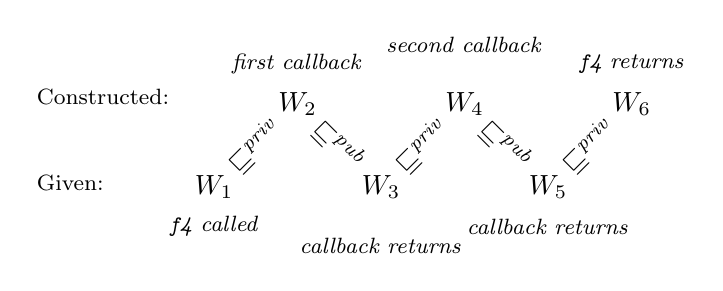
\begin{tikzpicture}[main node/.style={}, node distance=1.5cm]
  \node[main node] (1) {$W_1$};
  \node[main node] (label1) [below of=1,yshift=1cm] {\footnotesize{\textit{\texttt{f4} called}}};
  \node[main node,left] (given) [left of=1,yshift=0.05cm] {\parbox{1.5cm}{\footnotesize{Given:}}};

  \node[main node] (2) [above right of=1]{$W_2$};
  \node[main node] (label2) [above of=2,yshift=-1cm] {\textit{\footnotesize{first callback}}};

  \node[main node,left] (const) [above of=given,yshift=-0.4cm] {\parbox{1.5cm}{\footnotesize{Constructed:}}};

  \node[main node] (3) [below right of=2]{$W_3$};
  \node[main node] (label3) [below of=3,yshift=0.75cm] {\footnotesize{\textit{callback returns}}};

  \node[main node] (4) [above right of=3]{$W_4$};
  \node[main node] (label4) [above of=4,yshift=-0.75cm] {\footnotesize{\textit{second callback}}};

  \node[main node] (5) [below right of=4]{$W_5$};
  \node[main node] (label5) [below of=5,yshift=1cm] {\footnotesize{\textit{callback returns}}};

  \node[main node] (6) [above right of=5]{$W_6$};
  \node[main node] (label6) [above of=6,yshift=-1cm] {\footnotesize{\textit{\texttt{f4} returns}}};
  \path(1) edge[draw=none] node [sloped, auto=false, allow upside down] {$\sqsubseteq^\priv$} (2)
       (2) edge[draw=none] node [sloped, auto=false, allow upside down] {$\sqsubseteq^\pub$} (3)
       (3) edge[draw=none] node [sloped, auto=false, allow upside down] {$\sqsubseteq^\priv$} (4)
       (4) edge[draw=none] node [sloped, auto=false, allow upside down] {$\sqsubseteq^\pub$} (5)
       (5) edge[draw=none] node [sloped, auto=false, allow upside down] {$\sqsubseteq^\priv$} (6);
\end{tikzpicture}
\caption{Illustration of the worlds in the proof of
  Lemma~\ref{lem:correctness-g1}. In the proof, the top row of worlds are
  constructed by us, while the bottom row of worlds are given. $W_6$ is constructed such
  that $W_6 \futurestr W_5$ \emph{ and } $W_6 \futurewk W_1$.}
  \label{fig:worlds-in-pf-g1}
\end{figure}

\begin{comment}
\begin{itemize}
\item Ticket dispenser
\item The awkward example and variants
\item A sandboxing example?

For example, an untrusted advertisement scenario with initialization code
that registers a redraw callback. The redraw callback gets temporary
read-write access to a framebuffer.

\item Some compartmentalization result?
\end{itemize}
\end{comment}

\section{Discussion}
\label{sec:discussion}
\itoplassug{Reviewer C, esop, would have liked a discussion of (a) what could be done on a machine with a smaller set of capabilities, e.g., no local capability (we could probably not have done anything as the stack pointer could be stored on the heap and reused at unintended times.) and (b) what could be done with a larger/stronger set of available capabilities (we could include a discussion of linear capabilities).}
\itoplassug{Reviewer C, esop, asks whether our attacker model is reasonable (see tex comment). Maybe we should include a short discussion of the attacker model.}
% p.18 "they are linked with an adversary, adv, that is allowed to allocate memory but has no other capabilities".  Is this a reasonable model of the adversary?  (Genuinely naive question.)
\itoplassug{Should we include a discussion of how this ``scales'' to other things like a multi-core setting or if we needed tail calls?}
% * Also, the local capabilities seem related to Boyland's "Borrowing"
%   e.g. that is now supported in Rust amongst other research languages
%   (Pony etc) also mentioned in the ECOOP paper.
% * the combination of E and L capabilities seems very interesting
%   indeed.  I wonder if e.g. they could be used to support strong
%   models of encapsulation e.g. like ownership types. (see eg LNCS
%   7850)
\noindent\textbf{Calling convention}\\
\emph{Formulating control flow correctness} While we claim that our calling
convention enforces control-flow correctness, we do not prove a general theorem
that shows this, because it is not clear what such a theorem should look like.
Formulations in terms of a control-flow graph, like the one by \citet{abadi_control-flow_2005}, do not take into account temporal properties,
like the well-bracketedness that Example~\texttt{\footnotesize{g1}} relies on.
In fact, our examples show that our logical relation imply a stronger form of
control-flow correctness than such formulations, although this is not made very
explicit. As future work, we consider looking at a more explicit and useful way
to formalize control-flow correctness. The idea would be to define a variant
of our capability machine with call and return instructions and
well-bracketed control flow built-in to the operational semantics, and then
prove that compiling such code to our machine using our calling convention is
fully abstract~\citep{abadi_protection_1998}.
\itoplassug{Maybe elaborate on why full-abstractness and not weaker properties like ``robust safety''.}

\emph{Performance and the requirement for stack clearing} The additional
security measures of the calling convention described in
\sectionname~\ref{sec:stack-and-return-pointer} impose an overhead compared to a
calling convention without security guarantees. However, most require only a few
atomic checks or register clearings on boundary crossings between trusted code
and adversary, which should produce an acceptable performance overhead. The only
exception are the requirements for stack clearing that we have in two
situations: when returning to the adversary and when invoking an adversary
callback. As we have explained, we need to clear all of the stack that we are
not using ourselves, not just the part that we have actually used. In other
words, on every boundary cross between trusted code and adversary code, a
potentially large region of memory must be cleared.

First, contrary to what we explained before, we actually suspect that this overhead can be avoided in one of the two cases: when returning to the adversary.
In that case, we now think it would suffice to clear only the (much smaller) part of the stack used by the trusted code itself.
To understand this, it is useful to take another look at the illustrations in Figure~\ref{fig:ret-adv} related to this case.
If we do not clear the stack upon return (as illustrated in Figure~\ref{fig:illu-clear-all}), then the adversary might have used that stack to store local capabilities they received in a previous invocation (see Figure~\ref{fig:illu-adv-data}).
In other words, the stack clearing is necessary for revoking those local capabilities: the stack pointer and return pointer for the invocation illustrated in Figure~\ref{fig:illu-adv-data}.
While this approach is safe, we now suspect that we could do without the revocation in this case.
The stack pointer which the adversary was given access to in the stack frame depicted in Figure~\ref{fig:illu-call-adv} only carries authority that the adversary has access to in the higher stack frame anyway.
Similarly, the return pointer is merely an entry pointer pointing into the trusted code's stack frame, and this is also a capability that the adversary we return to could have constructed themselves from their stack pointer.

This improvement of our calling convention is a recent insight and not yet reflected in our examples and our proofs.
We do believe the proofs could be updated to accomodate for this change, but it would require some non-trivial changes.
Consider the awkward example proof, for example, we would have to ensure that the world $W_6$, depicted in Figure~\ref{fig:worlds-in-pf-g1} would not just be a private future world of $W_5$, but a public one (in addition to being a public future world of $W_1$).
This would allow us to do without the stack clearing, but it would entail some changes to the islands we use, and an extra argument that the old adversary's stack and return pointer remain valid after clearing the trusted code's stack frame and relaxing the invariant that used to ensure it could not be modified.
While this change is a clear improvement, we do not actually believe that it fundamentally changes the efficiency characteristics of the approach: the cost is halved, but remains asymptotically the same.

A second important remark we want to make is that the need for stack clearing in our calling convention is an instance of a general caveat when using CHERI's local capabilities as a restricted form of capability revocation.
Consider how our use of local capabilities can be interpreted as temporarily delegating the stack and return capability to callees and then revoking the granted authority after the callee returns.
From this perspective, local capabilities are a general feature enabling this temporary delegation of authority for the duration of an invocation and this is also how they are described by the authors~\citep{Watson2015Cheri}.
However, our requirement for stack clearing on boundary crossings is also general.
Revoking authority that was granted temporarily using local capabilities, requires clearing all memory for which the invokee had write-local authority (or at least erasing all local capabilities from that memory).
Without micro-architectural support for efficiently clearing large ranges of memory, local capabilities can only be used for revocation in scenarios where the duration of a revocation is unimportant or the adversary only has write-local access to small amounts of memory.
In future work, we are planning to investigate an alternative notion of \emph{linear} capabilities that offer a limited form of revocation without such limitations.

Note, by the way, that CheriBSD's use of local capabilities in ccall does not actually involve a form of revocation.
CheriBSD's model involves a trusted stack manager that gives every compartment access to its own private stack using a local, write-local capability \citep{Watson2015Cheri}.
The locality of the stack capability allows the trusted stack manager to prevent compartments from leaking their stack pointer in a boundary crossing, but those capabilities are never actually revoked.
In fact, a compartment can easily store away such local capabilities in its own private stack and recover them there during future invocations.

Since local capabilities seem intended to provide a restricted form of revocation, perhaps capability machines like CHERI should consider to provide special support for this requirement.
Ideally, such support would take the form of a highly-optimized instruction for erasing a large block of memory.
However, from a discussion with the designers of the CHERI capability machine, we gather that it is not immediately clear whether and how such a primitive could be implemented efficiently in the CHERI context.
\itoplassug{Maybe refer to some of the papers
  reviewer A, esop mentions for stack clearing. See comment in tex file. }
% http://scale.eecs.berkeley.edu/papers/mmp-asplos2002.pdf
% https://www.usenix.org/legacy/event/osdi08/tech/full_papers/zeldovich/zeldovich_html/index.html
% http://users.ece.utexas.edu/~tiwari/pubs/MICRO-08-rangecache.pdf

\emph{Modularity} It is important that our calling convention is modular, i.e.\
we do not assume that our code is specially privileged w.r.t.\ the adversary,
and they can apply the same measures to protect themselves from us as we do to
protect ourselves from them. More concretely, the requirements we have on
callbacks and return pointers received from the adversary are also satisfied by
callbacks and return pointers that we pass to them. For example, our return
pointers are local capabilities because they must point to memory where we can
store the old stack pointer, but the adversary's return pointers are also
allowed to be local. Adversary callbacks are required to be global but the
callbacks we construct are allocated on the heap and also global.

\emph{Arguments and local capabilities} 
%Stack and return pointer
%Local capabilities cannot be "freely used"
%Safety dictated by LR
%Need to dynamical check whether we overwrite our local stuff.
Local capabilities are a central part of the calling convention as they are used
to construct stack and return pointers. The use of local capabilities for the
calling convention unfortunately limits the extent to which local capabilities
can be used for other things. Say we are using the calling convention and
receive a local capability other than the stack and return pointer, then we need
to be careful if we want to use it because it may be an alias to the stack
pointer. That is, if we first push something to the stack and then write to the
local capability, then we may be (tricked into) overwriting our own local state.
The logical relation helps by telling us what we need to ascertain or check in
such scenarios to guarantee safety and preserve our invariants, but such checks
may be costly and it is not clear to us whether there are practical scenarios
where this might be realistic.

%Pass capability on
%Stack example
%Pass argument by reference
%Sofisticated deep safety analysis
We also need to be careful when we receive a capability from an adversary that
we want to pass on to a different (instance of the) adversary. It turns out that
the logical relation again tells us when this is safe. Namely, the logical
relation says that we can only pass on arguments that are safe in the world we
invoke the adversary in. For instance, when we receive a stack pointer from an
adversary, then we may at some point want to pass on part of this stack pointer
to, say, a callback. In order to do so, we need to make sure the stack pointer
is safe which means that, if we have revoked temporary invariants, the stack
must not directly or indirectly allow access to local values that we cannot
guarantee safety of. When received from an adversary, we have to consider the
contents of the stack unsafe, so before we pass it on, we have to clear it, or
perform a dynamic safety analysis of the stack contents and anything it points
to. Clearing everything is not always desirable and a dynamic safety analysis is
hard to get right and potentially expensive.

% Can local capabilities be used for other things?/Local capabilities only for stack?
%Not unheard of - other machine also have things specific for language features.
In summary, the use of local capabilities for other things than stack and return
pointers is likely only possible in very specific scenarios when using our
calling convention. While this is unfortunate, it is not unheard of that
processors have built-in constructs that are exclusively used for handling
control flow, such as, for example, the call and return instructions that exist
in some instruction sets.
% Old version of the above:
% Carefully constructing stack and return
% pointer plays a big part in the calling convention, but it is completely
% undermined if an unsafe argument, say the full stack pointer that include the
% caller's local stack frame, is passed as an argument of the call. The logical
% relation dictates when it is safe to pass an argument to an adversary, namely it
% must be a safe value. In order to illustrate what this means for local
% capabilities, consider the stack capability. When the stack capability is
% received from an adversary, then the contents of the stack is unknown and must
% thus be considered unsafe, so before the stack capability can be passed on, we
% must make sure that it only gives access to safe values. In order to meet this
% requirement, we take a conservative approcah and simply clear everything on the
% stack. Integers are always safe, so the stack capability can now safely be
% passed on. While this approach works for the stack, it may in practice be a bit
% too naive for other local capabilities received form an adversary. Say we
% receive a capability from an adversary that happens to be the first part of the
% stack. We want to pass this capability on, so we naively clear the contents it
% gives access to which in the worst case means we overwrite our local data or the
% activation record. While this is strictly speaking not unsafe (integers are
% always) safe, it is not desirable in a real system. We would in principle also
% like to be able to pass on arguments by reference, e.g a local capability for
% some array of values. In this case, it would not be satisfactory to just clear the
% entire thing. However, the capability still needs to be safe, so there would
% need to be some kind of deep dynamic check that ensures that everything the
% capability gives access to is indeed safe. In a real setting, this may again be
% undesirable.
% This also points to a more
% general problem: When can we use local capabilities we have received from an
% adversary. We at least need to do some kind of dynamic range check to make sure
% that we do not inadverdently overwrite our local stack frame.

\itoplassug{We could also include a brief discussion of concurrency and the fact that this probably wouldn't scale to it (but well-bracktedness is not the same in that case anyway.) }
\itoplassug{Reviewer C, esop, wants to know what happens when there are several stack blocks (see tex for comment). We could here emphasize that while we talk about a single stack there could be multiple local read/write-local/execute-capabilities. If we get the stack from an untrusted source, which is the case in the awkward example, then we will use anything that \emph{looks like} the stack as the stack. However, due to the operational semantics for local capabilities all other ``stack blocks'' would have to be stored on the stack or in the register file. As the calling convention dictates that we clear these, the only place the alternative stack blocks will not be cleared is on a part of the stack that we do not have access to. The return capability would basically have to encapsulate this part of memory (perhaps indirectly) which means that from the moment we have been called, we will make sure there is only one stack available until our program returns from the initial call to it.}
%p.10 "to prevent this from happening, we need to make sure the stack capability carries RWLX authority, since the system wide assumption then tells us that the adversary cannot have global capabilities to our local stack".  It feels like the "L" capabitility is being overloaded to mean not just "this memory block has write-local authority and can contain local capabilities", but also to mean "this memory block is my stack and no other block is".  What happens when there are several stack blocks, e.g. one per thread?
\emph{Single stack} A single stack is a good choice for the simple capability
machine presented here, because it works well with higher-order functions. An
alternative to a single stack would be to have a separate stack per component.
The trouble with this approach is that, with multiple stacks and local stack
pointers, it is not clear how components would retrieve their stack pointer upon
invocation without compromising safety. A safe approach could be to have stack
pointers stored by a central, trusted stack management component, but it is not
clear how that could scale to large numbers of separate components. Handling
large numbers of components is a requirement if we want to use
capability machines to enforce encapsulation of, for example, every object in an
object-oriented program or every closure in a functional program.
\\\\
\begin{toplas}
\noindent \textbf{Reasoning about capability machine programs}\\
\emph{Semantic, but not syntactic properties} The logical relation defined in
\sectionname~\ref{sec:logical-relation} allows us to reason about capability machine
programs. A limitation w.r.t. previous work is that the logical relation is
tailored exclusively towards semantic properties, not syntactic ones.

Imagine, for example, that we invoke a block of adversary code in such a way
that it only ever receives capabilities within a specific range of memory. After
the code returns, we may try to prove that any capabilities passed back to us in
the registers are still confined to that range of memory. The property of
falling in a certain address range is syntactic in the sense that it talks about
the specific implementation of a higher-order value rather than its behavior,
like the invariants that are required/preserved when we use it.

Such syntactic properties are hard to prove in our system. For the example
cited, it would be easy to conclude that the returned values are in the value
relation (see \figurename~\ref{fig:logrel}). This gives us a lot of semantic
information, like conditions under which they are safe to use and invariants
that will be preserved when we do, but it does not tell us much about the
address of the capability. As a very concrete example, capabilities with
permission $\noperm$ are always in the value relation, irrespective of their
address. Semantically, this makes perfect sense, since they are always safe
since they cannot be used for anything anyway. However, it also means we do not
get syntactic information about them.

For our purposes, this restriction is unproblematic, since we are only
interested in proving semantic properties (e.g., an assertion will never fail).
However, in other situations, we may be interested in proving more syntactic
properties like the ones that are often considered in object capability
literature: confinement, no authority amplification etc. Although such
properties are more restrictive and less easy to use for reasoning,
\citet{Devriese:2016ObjCap} have demonstrated how a logical relation like
ours can be adapted to also support them, by quantifying the logical relation
over a custom interpretation of effectful computations and the type of
references. We expect their solution can be readily adapted to our setting,
modulo some details (like the fact that we do not just have read-write
capabilities, but also others).
\end{toplas}
% % \emph{No program logic} TODO: discuss this? 
\\\\
\noindent\textbf{Logical relation}\\
\emph{Single orthogonal closure} The definitions of $\stder$ and $\stdvr$ in
\figurename~\ref{fig:logrel} apply a single orthogonal closure, a new variant of an
existing pattern called biorthogonality. Biorthogonality is a pattern for
defining logical relations~\citep{krivine_classical_1994,pitts_operational_1998}
in terms of an observation relation of safe configurations (like we do). The
idea is to define safe evaluation contexts as the set of contexts that produce
safe observations when plugging safe values and define safe terms as the set of
terms that can be plugged into safe evaluation contexts to produce safe
observations. This is an alternative to more direct definitions where safe terms
are defined as terms that evaluate to safe values. An advantage of
biorthogonality is that it scales better to languages with control effects like
call/cc. Our definitions can be seen as a variant of biorthogonality, where we
take only a single orthogonal closure: we do not define safe evaluation contexts
but immediately define safe terms as those that produce safe observations when
plugged with safe values. This is natural because we model arbitrary assembly
code that does not necessarily respect a particular calling convention: return
pointers are in principle values like all others and there is no reason to treat
them specially in the logical relation.

Interestingly, \citet{Hur:2011:KLR:1926385.1926402} also use a step-indexed,
Kripke logical relation for an assembly language (for reasoning about correct
compilation from ML to assembly), but because they only model non-adversarial
code that treats return pointers according to a particular calling convention,
they can use standard biorthogonality rather than a single orthogonal closure
like us.


\emph{Public/private future worlds} A novel aspect of our logical relation is
how we model the temporary, revokable nature of local capabilities using public/private
future worlds. The main insight is that this special nature generalizes that of the syntactically-enforced
unstorable status of evaluation contexts in lambda calculi without control
effects (of which well-bracketed control flow is a consequence). To reason about
code that relies on this (particularly, the original awkward example),
\citet{Dreyer:jfp12} (DNB) formally capture the special status of evaluation
contexts using Kripke worlds with public and private future world relations.
Essentially, they allow relatedness of evaluation contexts to be monotone with
respect to a weaker future world relation (public) than relatedness of values,
formalizing the idea that it is safe to make temporary internal state
modifications (private world transitions, which invalidate the continuation,
but not other values) while an expression is performing internal steps, as long
as the code returns to a stable state (i.e. transitions to a public future world
of the original) before returning. We
generalize this idea to reason about local capabilities: validity of local
capabilities is allowed to be monotone with respect to a weaker future-world
relation than other values, which we can exploit to distinguish between state
changes that are always safe (public future worlds) and changes that are only
valid if we clear all local capabilities (private future worlds). Our future
world relations are similar to DNB's (for example, our proof of
the awkward example uses exactly the same state transition system),
but they turn up in an entirely different place in the logical relation: rather
than using public future worlds for the special syntactic category of evaluation
contexts, they are used in the value relation depending on the
locality of the capability at hand. Additionally, our worlds are a bit more
complex because, to allow local memory capabilities and write-local
capabilities, they can contain (revokable) temporary regions that are only
monotonous w.r.t. public future worlds, while DNB's worlds are entirely
permanent.

\emph{Local capabilities in high-level languages} We point out that
local capabilities are quite similar to a feature proposed for the high-level
language Scala: \citet{osvald_gentrification_2016}'s second-class or local
values. They are a kind of values that can be provided to other code for
immediate use without allowing them to be stored in a closure or reference for
later use. We believe reasoning about such values will require techniques similar 
to what we provide for local capabilities.

\itoplassug{Reviewer C, popl, would like to know how local capabilities relate to borrowing (see tex comment).}

\section{Related Work}
\label{sec:related-work}

Finally, we summarize how our work relates to previous work. We do not
repeat the work we discussed in \sectionname~\ref{sec:discussion}.

Capability machines originate with \citet{Dennis:1966:PSM:365230.365252} and we refer to \citet{Levy1984capability} and \citet{Watson2015Cheri} for an overview
of previous work. The capability machine formalized in
\sectionname~\ref{sec:capab-mach-with} is a simple but representative
model, modeled mainly after the
M-Machine~\citep{Carter:1994:HSF:195473.195579} (the enter pointers
resemble the M-Machine's) and
CHERI~\citep{Watson2015Cheri,Woodruff:2014:CCM:2665671.2665740} (the
memory and local capabilities resemble CHERI's). The latter is a
recent and relatively mature capability machine, which combines
capabilities with a virtual memory approach, in the interest of
backwards compatibility and gradual adoption. As discussed, our local
capabilities can cross module boundaries, 
contrary to what is enforced by CHERI's default CCall implementation.

Plenty of other papers\lau{If there are plenty, then I guess we should cite more
  than one?} enforce well-bracketed control flow at a low level, but most are
restricted to preventing particular types of attacks and enforce only partial
correctness of control flow. This includes particularly the line of work on
\emph{control-flow integrity}~\citep{abadi_control-flow_2005}. Those use a quite
different attacker model than us: they assume an attacker that is not able to
execute code, but can overwrite arbitrary data at any time during execution (to
model buffer overflows). By checking the address of every indirect jump and
using memory access control to prevent overwriting code, this work enforces what
they call control-flow integrity, formalized as the property that every jump
will follow a legal path in the control-flow graph. As discussed in
\sectionname~\ref{sec:discussion}, such a property ignores temporal properties and
seems hard to use for reasoning.

More closely related to our work are papers that use a trusted stack manager and
some form of memory isolation to enforce control-flow correctness as part of a
secure compilation
result~\citep{patrignani_modular_2016-1,juglaret_beyond_2016-1}. Our work
differs from theirs in that we use a different form of low-level security
primitive (a capability machine with local capabilities rather than a machine
with a primitive notion of compartments) and we do not use a trusted stack
manager, but a decentralized calling convention based on local
capabilities. Also, both prove a secure compilation result from a high-level
language, which clearly implies a general form of control-flow correctness,
while we define a logical relation that can be used to reason about
specific programs that rely on well-bracketed control flow.

\lau{Reviewer C, esop, would like a better comparison with \citet{Devriese:2016ObjCap} (but also admits that they did not follow the below discussion).}
Our logical relation is a unary, step-indexed Kripke logical relation with
recursive worlds
\citep{pitts_operational_1998,Appel:2001:IMR:504709.504712,Ahmed2004semantics,Birkedal:2011:SKM:1926385.1926401},
closely related to the one used by \citet{Devriese:2016ObjCap} to formulate
capability safety in a high-level JavaScript-like lambda calculus. Our
Fundamental Theorem is similar to theirs and expresses capability safety of the
capability machine. Because we are not interested in externally observable
side-effects (like console output or memory access traces), we do not require
their notion of effect parametricity. Our logical relation uses several ideas
from previous work, like Kripke worlds with regions containing state transition
systems \citep{Ahmed:popl09}, public/private future worlds \citep{Dreyer:jfp12}
(see \sectionname~\ref{sec:discussion} for a discussion), and biorthogonality
\citep{pitts_operational_1998,benton_biorthogonality_2009-1,Hur:2011:KLR:1926385.1926402}.

\citet{swasey:2017} have recently developed a \emph{logic}, OCPL, for verification
of object capability patterns. The logic is based on
Iris~\citep{iris,iris2,iris3}, a state of the art higher-order concurrent
separation logic and is formalized in Coq, building on the Iris Proof Mode for
Coq~\citep{ipm}. OCPL gives a more abstract and modular way of proving
capability safety for a lambda-calculus (with concurrency) compared to the
earlier work by \citet{Devriese:2016ObjCap}.
% domi: rest of the paragraph could be cut?
\begin{toplas}
In the future we would also like to investigate a new program logic for
reasoning about capability safety for our capability machine model. In fact,
we think the lemmas in Section~\ref{sec:reasoning} are suggestive of the style
of results that could be written in such a logic. We think Iris would also be
a natural starting point for such an endeavour, since Iris is really a
framework, which can be instantiated to different programming languages. OCPL
was able to leverage existing Iris specifications for the high-level language;
for our capability machine model, however, it would be necessary to devise new
kinds of specifications for our low-level programs with unstructured
control-flow. It is likely that we could get inspiration from earlier work on
logics for assembly programming languages, such as XCAP~\citep{xcap}.
\end{toplas}
\itoplassug{We could further add that this is not the level of abstraction that one would like to reason. One would like to reason about the programs we actually write - that is programs written in high-level languages. If we had a fully-abstract compiler from a nice high-level language to this low-level machine, then we could reason about the program in the high-level language and then because the compiler is fully-abstract, we would retain all the nice properties from the high-level language. How does this work fit in to this picture? The calling convention ensures two properties that we expect our nice high-level languages to have, namely well-bracketedness and local-state encapsulation. If we want to do fully-abstract compilation, then we need some way to guarantee this after compilation. Further, logical relations are often used in full-abstractness proofs. This work expands our knowledge about logical relations should be defined for low-languages and in particular capability machines. (maybe also mention that enforcement necessary for fully-abstract compilation. Could be capability, but it could also be something else - we just need something which we do not have now.)  }

El-Korashy also defined a formal model of a capability machine, namely CHERI,
and uses it to prove a compartmentalization
result~\citep{akram_el-korashy_formal_2016} (not implying control-flow
correctness). He also adapts control-flow integrity (see above) to the machine
and shows soundness, seemingly without relying on capabilities.

% \begin{acks}
% This research was supported in part by the ModuRes Sapere Aude Advanced Grant
% from The Danish Council for Independent Research for the Natural Sciences (FNU). 
% Support for an STSM was received from COST Action EUTypes (CA15123).
% Dominique Devriese holds a Postdoctoral fellowship from the Research Foundation Flanders (FWO).
% \end{acks}

%% Acknowledgments
% \begin{acks}                            %% acks environment is optional
%                                         %% contents suppressed with 'anonymous'
%   %% Commands \grantsponsor{<sponsorID>}{<name>}{<url>} and
%   %% \grantnum[<url>]{<sponsorID>}{<number>} should be used to
%   %% acknowledge financial support and will be used by metadata
%   %% extraction tools.
%   This material is based upon work supported by the
%   \grantsponsor{GS100000001}{National Science
%     Foundation}{http://dx.doi.org/10.13039/100000001} under Grant
%   No.~\grantnum{GS100000001}{nnnnnnn} and Grant
%   No.~\grantnum{GS100000001}{mmmmmmm}.  Any opinions, findings, and
%   conclusions or recommendations expressed in this material are those
%   of the author and do not necessarily reflect the views of the
%   National Science Foundation.
% \end{acks}


%% Bibliography
\bibliography{references}


%% Appendix
\appendix
\section{Appendix}
In this appendix, we give more precise formulations of lemmas that were mentioned in the paper, and the most important supporting definitions and lemmas.
The goal is to provide details that can help to understand in more detail what we discuss in the paper. 
Full details and proofs are not given here, but for those we refer to the technical appendix~\citep{technical_appendix}.

\subsection{Logical relation}
\label{app:logical-relation}
% Text of appendix \ldots
\textbf{$n$-subset simulation}
\begin{mathpar}
  \inferrule{(s,\phi_\pub,\phi) = (s',\phi_\pub',\phi') \\
    \forall \hat{W} \ldotp H \; s \; \hat{W} \nsubeq H' \; s' \; \hat{W} }
  { (v,s,\phi_\pub,\phi,H) \nsubsim (v',s',\phi_\pub',\phi',H')}
\end{mathpar}
%
\textbf{Transition system relations}
\begin{align*}
   \Rels &= \{(\phi_\pub, \phi) \in \powerset{\States^2}\times \powerset{\States^2} \mid \phi_\pub, \phi \text{ is reflexive and transitive and } \phi_\pub \subseteq \phi \}
\end{align*}
%
\textbf{Erasure}
\begin{align*}
  \lfloor W \rfloor_S \defeq \lambda r \ldotp 
  \begin{cases}
    W(r) & W(r).v \in S\\
    \bot & \text{otherwise}
  \end{cases}
\end{align*}
%
\textbf{Active region projection}
\begin{align*}
  \activeReg{} & : \Worlds \fun 2^\RegionNames \\
  \activeReg{W} & \defeq \dom(\erase{W}{\perma,\temp})
\end{align*}
%
\textbf{Projection of regions based on locality}
\[
  \localityReg(\gl,W) \defeq 
  \begin{cases}
    \dom(\erase{W}{\perm,\temp}) & \text{if } \gl = \local \\
    \dom(\erase{W}{\perm}) & \text{if } \gl = \glob
  \end{cases}
\]
%
\textbf{Address stratification}
\begin{align*}
&\iota = (v,s,\phi_\pub,\phi,H) \text{ is address-stratified iff }\\
&\qquad\begin{multlined}
  \forall s', \hat{W}, n, \ms, \ms' \ldotp \\
  \npair{\ms},\npair{\ms'} \in H~ s'~ \hat{W} \Rightarrow \\
  \dom(\ms) = \dom(\ms') \wedge \\
  \forall \addr \in
  \dom(\ms)\ldotp \npair{\ms\update{\addr}{\ms'(\addr)}} \in H~ s'~ \hat{W}
\end{multlined}
\end{align*}


\subsection{Complete ordered family of equivalences (c.o.f.e)}
\newcommand{\seq}[1]{\ensuremath{\left\{#1_n\right\}_{n=0}^{\infty}}}
\newcommand{\seqn}[1]{\ensuremath{\left(#1\right)_{n=0}^{\infty}}}
\newcommand{\NN}{\ensuremath{\mathbb{N}}}
\newcommand{\Ul}{\ensuremath{\mathcal{U}}}
\newcommand{\Later}{\ensuremath{\blacktriangleright}}
\newcommand{\op}[1]{\ensuremath{#1^{\text{op}}}}
\newcommand{\comp}{\circ}
\newcommand{\iso}{\cong}
\renewcommand{\hom}[3]{#1(#2,#3)}

\label{app:cofe}
This is an excerpt from \citet{Birkedal:tutorial-notes} about c.o.f.e.'s.
\begin{definition}[o.f.e.] An \emph{ordered family of equivalence} (o.f.e) is a
  set and a family of equivalences $\left(X, \left( \nequal \right)_{n=0}^\infty
  \right)$ that satisfy the following properties: 
  \begin{itemize}
  \item $\nequal[0]$ is the total relation on $X$
  \item $\forall n \ldotp \forall x,y \in X \ldotp x \nequal[n+1] y \Rightarrow
    x \nequal y$
  \item $\forall x,y \in X \ldotp (\forall n\ldotp x \nequal y) \Rightarrow x = y$
  \end{itemize}
  We say that an o.f.e. $\left(X, \seqn{\nequal{n}}\right)$ is \emph{inhabited} if there
  exists an element $x \in X$.
\end{definition}

If you are familiar with metric spaces observe that o.f.e.'s are but a different
presentation of bisected $1$-bounded ultrametric spaces.

\begin{definition}[Cauchy sequences and limits]
  \label{def:cauchy-sequence}
  Let $\left(X, \seqn{\nequal} \right)$ be an o.f.e. and $\seq{x}$ be a sequence of
  elements of $X$. Then $\seq{x}$ is a \emph{Cauchy sequence} if
  \begin{align*}
    \forall k \in \nats, \exists j \in \nats, \forall n \geq j, x_j \nequal{k} x_n
  \end{align*}
  or in words, the elements of the chain get arbitrarily close.

  An element $x \in X$ is the \emph{limit} of the sequence $\seq{x}$ if
  \begin{align*}
    \forall k \in \nats, \exists j \in \nats, \forall n \geq j, x \nequal{k} x_n.
  \end{align*}
  A sequence may or may not have a limit. If it has we say that the sequence
  \emph{converges}. The limit is necessarily unique in this case
  and we write $\lim_{n\to\infty}x_n$ for it.
\end{definition}

\begin{definition}[c.o.f.e.] A \emph{complete} ordered family of equivalences
  (c.o.f.e) is an o.f.e $\left(X, \left( \nequal \right)_{n=0}^\infty \right)$
  where all Cauchy sequences have a limit.  
\end{definition}

\begin{definition}
  \label{def:nonexpansive-contractive-ofe}
  Let $\left(X, \seqn{\nequal_{X}}\right)$ and $\left(Y, \seqn{\nequal_{Y}}\right)$ be
  two ordered families of equivalences and $f$ a function from the set $X$ to the set $Y$.
  The function $f$ is 
  \begin{itemize}
  \item \emph{non-expansive} if for any $x, x' \in X$, and any $n \in \nats$,
    \begin{align*}
      x \nequal_X x' \implies f(x) \nequal_Y f(x')
    \end{align*}
  \item \emph{contractive} if for any $x, x' \in X$, and any $n \in \nats$,
    \begin{align*}
      x \nequal_X x' \implies f(x) \nequal[n+1]_Y f(x')
    \end{align*}
  \end{itemize}
\end{definition}

\begin{theorem}[Banach's fixed point theorem]
  \label{thm:banach-fixed-point}
  Let $\left(X, \seqn{\nequal}\right)$ be a an inhabited c.o.f.e. and $f : X \to X$ a contractive
  function. Then $f$ has a unique fixed point.
\end{theorem}

\begin{definition}[The category $\Ul$]
  The category $\Ul$ of complete ordered families of equivalences has as objects complete
  ordered families of equivalences and as morphisms non-expansive functions.
\end{definition}

\begin{definition}
  \label{def:later-functor}
  The functor $\Later$ is a functor on $\Ul$ defined as
  \begin{align*}
    \Later\left(X, \seqn{\nequal}\right) &= \left(X,
          \seqn{\overset{n}{\equiv}}\right)\\
    \Later(f) &= f
  \end{align*}
  where $\overset{0}{\equiv}$ is the total relation and $x \overset{n+1}{\equiv} x'$
  iff $x \nequal x'$
\end{definition}

From now on, we often use the underlying set $X$ to denote a (complete) o.f.e. $\left(X,
  \seqn{\nequal}\right)$, leaving the family of equivalence
relations implicit.

\begin{definition}
 \label{def:nonexpansive-loc-contractive-functor}
 A functor $F : \op{\Ul} \times \Ul \to \Ul$ is \emph{locally non-expansive}  if for all
 objects $X$, $X'$, $Y$, and $Y'$ in $\Ul$ and
 $f, f' \in \hom{\Ul}{X}{X'}$ and $g, g' \in \hom{\Ul}{Y'}{Y}$ we have
 \begin{align*}
   f \overset{n}{=} f' \land g \overset{n}{=} g' \implies F(f, g) \overset{n}{=} F(f', g').
 \end{align*}

 It is \emph{locally contractive} if the stronger implication
 \begin{align*}
   f \overset{n}{=} f' \land g \overset{n}{=} g' \implies F(f, g) \overset{n+1}{=} F(f', g').
 \end{align*}
 holds. Note that the equalities are equalities on function spaces.
\end{definition}

\begin{proposition}
  \label{prop:loc-nonexp-loc-contr}
  If $F$ is a locally non-expansive functor then $\Later \comp F$ and $F \comp \left(\op{\Later}
  \times \Later\right)$ are locally contractive. Here, the functor $F \comp \left(\op{\Later} \times
  \Later\right)$ works as
  \begin{align*}
    (F \comp (\op{\Later} \times \Later))(X, Y) = F\left(\op{\Later}(X), \Later(Y)\right)
  \end{align*}
  on objects and analogously on morphisms and
  $\op{\Later} : \op{\Ul} \to \op{\Ul}$ is just $\Later$ working on $\op{\Ul}$ (i.e., its
  definition is the same).
\end{proposition}

\begin{definition}
 \label{def:fixed-point}
 A fixed point of a locally contractive functor $F$ is an object $X \in \Ul$, such that
 $F(X, X) \iso X$.
\end{definition}

The following is America and Rutten's fixed point theorem~\citep{America-Rutten:JCSS89}.
\begin{theorem}
 \label{thm:contr-functors-have-fixed-points}
 Every locally contractive functor $F$ such that $F(1, 1)$ is inhabited has a unique fixed
 point. The fixed point is unique among inhabited c.o.f.e.'s.
 If in addition $F(\emptyset, \emptyset)$ is inhabited then the fixed point of $F$ is unique.
\end{theorem}
In~\citet{BirkedalL:metric-enriched-journal} one can find a
category-theoretic generalization, which shows how to obtain fixed
points of locally contractive funtors on categories enriched in $\Ul$,
in particular on the category of preordered c.o.f.e.'s.  A preodered c.o.f.e. is
a c.o.f.e. equipped with a preorder that is closed under taking limits of
converging sequences.
The formulation in \emph{loc. cit.} also applies to solve
mutually recursive domain equations on preordered c.o.f.e.'s; see~\citet{bizjak:mutually-recursive-mcat}
for an explicit statement. That is the solution theorem we use to prove
Theorem~\ref{thm:world-existence}.



\subsection{Load instruction sufficiency lemma}
 \begin{lemma}[Conditions for store instruction are sufficient]
   \label{lem:conds-store-suff}
   If 
   \begin{itemize}
   \item $\ms = \ms' \uplus \ms_f$
   \item $\heapSat[\ms']{n}{W}$
   \item $((\perm,\gl),\start,\addrend,\addr) = c$
   \item $\npair{c}\in\stdvr(W)$
   \item $\writeAllowed{\perm}$
   \item $\withinBounds{\var{c}}$
   \item $\npair{\var{w}}\in\stdvr(W)$
   \item if $\var{w} = ((\_,\local),\_,\_,\_)$, then $\perm \in
     \{\rwlx,\readwritel \}$
   \end{itemize}
 
   then $\addr \in \dom(\ms')$ (i.e. $\ms\update{a}{w} =
   \ms'\update{a}{w}\uplus\ms_f$) and
   $\heapSat[{\ms'\update{\addr}{\var{w}}}]{n}{W}$
 \end{lemma}


\subsection{Macros}
Implementation of the macros used in \texttt{scall}. Implementations of the
macros not presented here can be found in the technical
appendix~\citep{technical_appendix}.\\
\label{app:macros}
\texttt{push $r$}
\begin{lstlisting}
  lea r_stk 1
  store r_stk r
\end{lstlisting}
\texttt{pop $r$}
\begin{lstlisting}
  load r r_stk
  minus r_t1 0 1
  lea r_stk r_t1
\end{lstlisting}
\texttt{rclear $r_1,\dots, r_n$}
\begin{lstlisting}
move $r_1$ 0
move $r_2$ 0
$\dots$
move $r_n$ 0
\end{lstlisting}
\texttt{mclear $r$}
\begin{lstlisting}
        move r_t $r$
        getb r_t1 r_t
        geta r_t2 r_t
        minus r_t2 r_t1 r_t2
        lea r_t r_t2
        gete r_t2
        minus r_t1 r_t2 r_t1
        plus r_t1 r_t1 1
        move r_t2 pc
        lea r_t2 $\var{ofc}_\var{end}$ 
        move r_t3 pc
        lea r_t3 $\var{ofc}_\var{iter}$
iter:
        jnz r_t2 r_t1
        store r_t 0
        lea r_t 1
        plus r_t1 r_t1 1
        jmp r_t3
end:
        move r_t 0
        move r_t1 0
        move r_t2 0
        move r_t3 0
\end{lstlisting}
Where $\var{ofc}_\var{end}$ and $\var{ofc}_\var{iter}$ are the offsets to the
label \texttt{end} % 9?
and \texttt{iter}, % 2?
respectively.

\subsection{Reasoning about programs definitions}
\begin{definition}
  We say that $(\reg,\ms) \text{ is looking at } [i_0,\cdots,i_n] \text{ followed by } c_{\mathit{next}}$ 
  iff
  \begin{itemize}
  \item $\reg(\pcreg) = ((p,g),b,e,a)$
  \item $p = \rwx$, $p = \exec$, or $p = \rwlx$
  \item $a+n\leq e$, $b\leq a\leq e$
  \item $\ms(a+0,\cdots,a+n) = [i_0,\cdots,i_n]$
  \item $c_{\mathit{next}} = ((p,g),b,e,a+n+1)$
  \end{itemize}
\end{definition}

\begin{definition}
  We say that ``\linksto{(\reg,\ms)}{\var{key}}{j}{c_\malloc}'' 
  iff
  \begin{itemize}
  \item $\reg(pc) = \stdcap$
  \item $\ms(\start) = ((\_,\_),\start_\link,\_,\_)$
  \item $\ms(\start_\link+j) = c$
  \end{itemize}
\end{definition}

\begin{definition}
  We say that $\reg \text{ points to stack with $\ms_\stk$ used and $\ms_{\mathit{unused}}$ unused}$
  iff
  \begin{itemize}
  \item $\reg(r_\stk) =((\rwlx,\local),b_\stk,e_\stk,a_\stk)$
  \item $\dom(\ms_{\mathit{unused}}) = [a_\stk+1,\cdots,e_\stk]$
  \item $\dom(\ms_\stk) = [b_\stk,\cdots,a_\stk]$ \lau{Maybe make it clear what happens when $\ms_\stk$ is empty}
  \item $b_\stk - 1\leq a_\stk$
  \end{itemize}
\end{definition}


 \subsection{Example correctness lemmas}
\begin{lemma}[Correctness lemma for \texttt{f1}, copy of Lemma~\ref{lem:correctness-f1}] \forcenewline
  \label{lem:correctness-f1-app}
  For all $n \in \nats$
  let
  \begin{align*}
    c_{\var{adv}} & \defeq ((\entry,\glob),\start_{\adv},\addrend_{\adv},\start_{\adv}+\olf) \\
    c_{f1} & \defeq ((\rwx,\glob),\mathtt{f1}-\olf,\mathtt{1f},\mathtt{f1}) \\
    c_\malloc & \defeq ((\entry,\glob),\start_\malloc,\addrend_\malloc,\start_\malloc+\olf) \\
    m & \defeq \hs_{f1} \uplus 
        \hs_\flag \uplus                
        \ms_{\var{link}} \uplus 
        \hs_\adv \uplus 
        \ms_{\malloc} \uplus 
        \hs_{\var{frame}} 
  \end{align*}
  and
  \begin{itemize}
  \item $c_\malloc$ satisfies the specification for malloc and $\iota_{\malloc,0}$ is the region from the specification.
  \end{itemize}
  where 
  \begin{align*}
    &\dom(\hs_{f1}) = [\mathtt{f1}-\olf,\mathtt{1f}] \\
    &\dom(\hs_\flag) = [\flag,\flag] \\
    &\dom(\ms_\link) = [\link,\link+1]\\
    &\dom(\hs_{\adv}) = [\start_\adv,\addrend_\adv] \\
    &\heapSat[\hs_{\malloc}]{n}{[0 \mapsto \iota_{\malloc,0}]}
  \end{align*}
  and
  \begin{itemize}
  \item $\ms_{f1}(\mathtt{f1}-\olf) = ((\readonly,\glob),\link,\link+1,\link)$, $\ms_{f1}(\mathtt{f1}-\olf+1) = ((\readwrite,\glob),\flag,\flag,\flag)$, the rest of $\hs_{f1}$ contains the code of $f1$.
  \item $\ms_\flag = [\flag \mapsto 0]$
  \item $\ms_{\var{link}} = [\var{link} \mapsto c_\malloc, \var{link} + 1 \mapsto c_\adv]$
  \item $\hs_\adv$ contains a global read-only capability for $\hs_\link$ on its first address. The remaining cells of the memory segment only contain instructions.
  \end{itemize}
  if 
  \[
    (\reg\update{\pcreg}{c_{f1}},m) \step[n] (\halted,m'),
  \]
  then
  \[
    m'(\flag) = 0
  \]  
\end{lemma}

\begin{lemma}[Correctness lemma for \texttt{f2}, detailed version of Lemma~\ref{lem:correctness-f2}]
  \label{lem:correctness-f2-app}
  let
  \begin{align*}
    c_{\var{adv}} & \defeq ((\entry,\glob),\start_{\adv},\addrend_{\adv},\start_{\adv}+\olf) \\
    c_{f2} & \defeq ((\rwx,\glob),\mathtt{f2}-\olf,\mathtt{2f},\mathtt{f2}) \\
    c_\malloc & \defeq ((\entry,\glob),\start_\malloc,\addrend_\malloc,\start_\malloc+\olf) \\
    c_{\var{stk}} & \defeq ((\rwlx,\local),\start_\stk,\addrend_\stk,\start_\stk-1) \\
    c_\link & \defeq ((\readonly,\glob),\link,\link+1,\link)\\
    \reg & \in \Regs \\
    m & \defeq \hs_{f2} \uplus 
        \hs_\flag \uplus                
        \ms_{\var{link}} \uplus 
        \hs_\adv \uplus 
        \ms_{\malloc} \uplus 
        \ms_{\var{stk}} \uplus
        \ms_{\var{frame}} 
  \end{align*}
  and
  \begin{itemize}
  \item $c_\malloc$ satisfies the specification for malloc and $\iota_{\malloc,0}$ is the region from the specification.
  \end{itemize}
  where 
  \begin{align*}
    &\dom(\hs_{f2}) = [\mathtt{f2}-\olf,\mathtt{2f}] \\
    &\dom(\hs_\flag) = [\flag,\flag] \\
    &\dom(\ms_\link) = [\link,\link+1]\\
    &\dom(\ms_\stk) = [\start_\stk, \addrend_\stk]\\
    &\dom(\hs_{\adv}) = [\start_\adv,\addrend_\adv] \\
    &\heapSat[\hs_{\malloc}]{n}{[0 \mapsto \iota_{\malloc,0}]} \qquad \text{ for all $n \in \nats$}
  \end{align*}
  and
  \begin{itemize}
  \item $\ms_{f2}(\mathtt{f2}-\olf) = ((\readonly,\glob),\link,\link+1,\link)$, $\ms_{f2}(\mathtt{f2}-\olf+1) = ((\readwrite,\glob),\flag,\flag,\flag)$, the rest of $\hs_{f2}$ contains the code of $f2$.
  \item $\ms_\flag = [\flag \mapsto 0]$
  \item $\ms_{\var{link}} = [\var{link} \mapsto c_\malloc, \var{link} + 1 \mapsto c_\adv]$
  \item $\hs_\adv(\start_\adv) = c_\link$ and $\forall \addr \in [\start_\adv+1,\addrend]\ldotp \ms_\adv(a) \in \ints$
  \end{itemize}
  if 
  \[
    (\reg\update{\pcreg}{c_{f2}}\update{r_\stk}{c_\stk},m) \step[n] (\halted,m'),
  \]
  then
  \[
    m'(\flag) = 0
  \]  
\end{lemma}
\begin{lemma}[Correctness lemma for \texttt{f3}, detailed version of Lemma~\ref{lem:correctness-f3}]
  \label{lem:correctness-f3-detailed}
  For all $n \in \nats$
  let
  \begin{align*}
    c_{\var{adv}} & \defeq ((\entry,\glob),\start_{\adv},\addrend_{\adv},\start_{\adv}+\olf) \\
    c_{f3} & \defeq ((\rwx,\glob),\mathtt{f3}-\olf,\mathtt{3f},\mathtt{f3}) \\
    c_{\var{stk}} & \defeq ((\rwlx,\local),\start_\stk,\addrend_\stk,\start_\stk-1) \\
    c_\malloc & \defeq ((\entry,\glob),\start_\malloc,\addrend_\malloc,\start_\malloc+\olf) \\
    c_\link & \defeq ((\readonly,\glob),\link,\link+1,\link) \\
    \reg & \in \Regs \\
    m & \defeq \hs_{f3} \uplus 
        \hs_\flag \uplus                
        \ms_{\var{link}} \uplus 
        \hs_\adv \uplus 
        \ms_{\malloc} \uplus 
        \ms_{\var{stk}} \uplus
        \ms_{\var{frame}} 
  \end{align*}
  and
  \begin{itemize}
  \item $c_\malloc$ satisfies the specification for malloc.
  \end{itemize}
  where 
  \begin{align*}
    &\dom(\hs_{f3}) = [\mathtt{f3}-\olf,\mathtt{3f}] \\
    &\dom(\hs_\flag) = [\flag,\flag] \\
    &\dom(\ms_\link) = [\link,\link+1]\\
    &\dom(\ms_\stk) = [\start_\stk, \addrend_\stk]\\
    &\dom(\hs_{\adv}) = [\start_\adv,\addrend_\adv] \\
    &\heapSat[\hs_{\malloc}]{n}{[0 \mapsto \iota_{\malloc,0}]}
  \end{align*}
  and
  \begin{itemize}
  \item $\ms_{f3}(\mathtt{f3}-\olf) = ((\readonly,\glob),\link,\link+1,\link)$, $\ms_{f3}(\mathtt{f3}-\olf+1) = ((\readwrite,\glob),\flag,\flag,\flag)$, the rest of $\hs_{f3}$ contains the code of $f3$.
  \item $\ms_\flag = [\flag \mapsto 0]$
  \item $\ms_{\var{link}} = [\var{link} \mapsto c_\malloc, \var{link} + 1 \mapsto c_\adv]$
  \item $\hs_\adv(\start_\adv) = c_\link$ and all other addresses of $\ms_\adv$ contain instructions.
  \end{itemize}
  if 
  \[
    (\reg\update{\pcreg}{c_{f3}}\update{r_\stk}{c_\stk},m) \step[n] (\halted,m'),
  \]
  then
  \[
    m'(\flag) = 0
  \]  
\end{lemma}

 
 \begin{lemma}[Correctness of $g1$, detailed version of Lemma~\ref{lem:correctness-g1}]
  \label{lem:correctness-g1-detailed}
  For all $n \in \nats$
  let
  \begin{align*}
    c_{\var{adv}} & \defeq ((\rwx,\glob),\start_{\adv},\addrend_{\adv},\start_{\adv}+\olf) \\
    c_{g1} & \defeq ((\entry,\glob),\mathtt{g1}-\olf,\mathtt{4f},\mathtt{g1}) \\
    c_\stk & \defeq ((\rwlx,\local),\start_\stk,\addrend_\stk,\start_\stk-1) \\
    c_\malloc & \defeq ((\entry,\glob),\start_\malloc,\addrend_\malloc,\start_\malloc+\olf) \\
    c_\link & \defeq ((\readonly,\glob),\link,\link,\link) \\
    m & \defeq \hs_{g1} \uplus 
        \ms_\flag \uplus                
        \ms_\link \uplus 
        \ms_\adv \uplus 
        \ms_\malloc \uplus 
        \ms_\stk \uplus
        \ms_{\var{frame}} 
  \end{align*}
  where 
  \begin{itemize}
  \item $c_\malloc$ satisfies the specification for malloc with $\iota_{\malloc,0}$
  \end{itemize}
  \begin{align*}
    &\dom(\hs_{g1}) = [\mathtt{g1}-\olf,\mathtt{4f}] \\
    &\dom(\hs_\flag) = [\flag,\flag] \\
    &\dom(\ms_\link) = [\link,\link]\\
    &\dom(\ms_\stk) = [\start_\stk, \addrend_\stk]\\
    &\dom(\hs_{\adv}) = [\start_\adv,\addrend_\adv] \\
    &\heapSat[\hs_{\malloc}]{n}{[0 \mapsto \iota_{\malloc,0}]}
  \end{align*}
  and
  \begin{itemize}
  \item $\ms_{g1}(\mathtt{g1}-\olf) = ((\readonly,\glob),\link,\link,\link)$, $\ms_{g1}(\mathtt{g1}-\olf+1) = ((\readwrite,\glob),\flag,\flag,\flag)$, the rest of $\hs_{g1}$ contains the code of $g1$ immediately followed by the code of $f4$.
  \item $\ms_\flag = [\flag \mapsto 0]$
  \item $\ms_{\var{link}} = [\link \mapsto c_\malloc]$
  \item $\hs_\adv(\start_\adv) = c_\link$ and all other addresses of $\ms_\adv$ contain instructions.
  \item $\forall a \in \dom(\ms_\stk) \ldotp \ms_\stk(a) = 0$ %This condition could be weakened to \memSat{\ms_\stk}{[\iota^\pwl(\dom(\ms_\stk))]}
  \end{itemize}
  if 
  \[
    (\reg_0\update{\pcreg}{c_\adv}\update{r_\stk}{c_\stk}\update{r_1}{c_{g1}},m) \step[n] (\halted,m'),
  \]
  then
  \[
    m'(\flag) = 0
  \]  
\end{lemma}


\subsection{Awkward example}
\textbf{The region for $x$} The region $\iota_x$, is the region omitted from the proof sketch for the awkward example.
\figurename~\ref{fig:x-reg} illustrates the transition system of $\iota_x$.
  \begin{figure}[tb]
    \centering
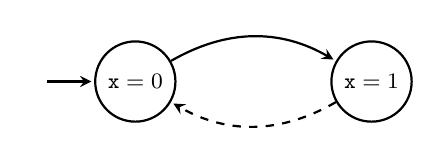
\begin{tikzpicture}[->,shorten >=1pt,auto,node distance=3cm,
  thick,main node/.style={circle,fill=white,draw,font=\sffamily\large},rect node/.style={rectangle,fill=blue!20,draw,font=\sffamily\large}]

  \node[main node] (n0) {\footnotesize $\texttt{x}=0$};
  \node (s) [left of=n0,xshift=1.75cm] {  };
  \node[main node] (n1) [right of=n0]  {\footnotesize $\texttt{x}=1$};
  \draw (s) edge[>=stealth] (n0);
  \draw (n0) edge[bend left,>=stealth] (n1);
  \draw (n1) edge[bend left,dashed,>=stealth] (n0);
  
\end{tikzpicture}
  \caption{Illustration of transition system in $\iota_x$. The dashed line is
    the private transition.}
  \label{fig:x-reg}
\end{figure}

\begin{definition}
  \label{def:iotax-region}
  \begin{align*}
    \iota_x   & = (\perm, 0, \phi_\pub, \phi, H_x) \\
    \phi_\pub & = \{(0,1)\}^* \\
    \phi      & = (1,0) \union \phi_\pub \\
    H_x \; s \; \hat{W} & = \{\npair{\ms} \mid \ms(x) = s \land n > 0 \} \union \{\npair[0]{\ms}\}
  \end{align*}
\end{definition}
\textbf{Static region} This static region only requires that the memory segment is the given one.
As it does not require safety, capabilities for this region cannot be gives to adversarial code.
\begin{align*}
  \iota^\sta (v,\ms) &= (v,1,=,=,H^\sta\;\ms)\\
  H^\sta \; \ms \; s \; \hat{W} = & \{\npair{\ms} \mid n > 0 \} \union \{\npair[0]{\ms'} \mid \ms' \in \Mems \}
\end{align*}
\textbf{Static safe region} Static region that also requires safety.
It is safe to give adversarial code read capabilities for this region.
\begin{align*}
  \iota^{\sta,u} (v,\ms) &= (v,1,=,=,H^{\sta,u}\;\ms)\\
  H^{\sta,u} \; \ms \; s \; \hat{W} = & \left\{\npair{\ms'} \middle|
    \begin{aligned}
      &\ms' = \ms \land\\
      &\forall \addr \in \dom(\ms) \ldotp\\
      & \quad \nonlocal{\ms(\addr)} \land\\
      & \quad \npair[n-1]{\ms(\addr)} \in \stdvr(\xi(\hat{W}))
    \end{aligned}
        \right\} \union \{\npair[0]{\ms'} \mid \ms' \in \Mems \}
\end{align*}


\end{document}
